\documentclass[a4paper,11pt,titlepage]{article}


% This first part of the file is called the PREAMBLE. It includes
% customizations and command definitions. The preamble is everything

\usepackage[margin=2cm]{geometry}  % set the margins to 2cm on all sides
\usepackage{graphicx}              % to include figures
\usepackage{amsmath}               % great math stuff
\usepackage{amsfonts}              % for blackboard bold, etc
\usepackage{amsthm}                % better theorem environments
\usepackage{wrapfig}					%allows wraping of figures in the text
\usepackage{cite}
\usepackage{bm}
\usepackage{natbib}
\usepackage{har2nat}
\usepackage{float}
%\usepackage{hyperref}

% various theorems, numbered by section

\newtheorem{thm}{Theorem}[section]
\newtheorem{lem}[thm]{Lemma}
\newtheorem{prop}[thm]{Proposition}
\newtheorem{cor}[thm]{Corollary}
\newtheorem{conj}[thm]{Conjecture}

\DeclareMathOperator{\id}{id}

\newcommand{\bd}[1]{\mathbf{#1}}  % for bolding symbols
\newcommand{\RR}{\mathbb{R}}      % for Real numbers
\newcommand{\ZZ}{\mathbb{Z}}      % for Integers
\newcommand{\col}[1]{\left[\begin{matrix} #1 \end{matrix} \right]}
\newcommand{\comb}[2]{\binom{#1^2 + #2^2}{#1+#2}}

\usepackage[nodayofweek]{datetime}
\usepackage{graphicx,subfig,listings}
\longdate

\usepackage{fancyhdr}
\pagestyle{fancyplain}
\fancyhf{}
\lhead{\fancyplain{}{Visualisation for Information -\ Sam Green}}
\rhead{\fancyplain{}{\today}}
\cfoot{\fancyplain{}{\thepage}}

\usepackage{url}

\title{Visualisation for Information: \\\ Deep Neural Networks \\\ \\\Large{--- Background and Progress Report ---}}
\author{Sam Green\\
       \small{sg5414@imperial.ac.uk}\\ \\
       \small{Supervisors: Dr William Knottenbelt and Mr Daniel `Jack' Kelly}
}

\begin{document}
\maketitle

\clearpage
\clearpage

\section*{Abstract}
A package, or platform designed to help experts in gaining deeper understanding of their artificial neural network models to diagnose potentially problematic issues with their model structure. This should allow for a more rapid iteration process as the researcher seeks to converge upon a well performing model.
\clearpage

\section*{Acknowledgments}
I would like to thank my supervisors Dr. William Knottenbelt and Mr. Daniel 'Jack' Kelly for their constant optimism, support and advice, my parents for their love and support, and the Turing Lab team who kept me sane throughout this project.

\clearpage

\tableofcontents
\clearpage

\section{Introduction}

	\subsection{Motivations}
	Deep Neural Networks are machine learning algorithms that enables incredibly accurate feature learning and hierarchical feature extraction. These algorithms were first employed decades ago, however made a strong comeback to the machine learning community in 2012 when in the ImageNET competition the clear winner by an unusual margin was a DNN. Since 2012 they have seen a dramatic increase in popularity in communities as far ranging as medicine, finance and sports prediction.
\par 
However unlike some machine learning models that are widely understood, such as logistic regression techniques, no one fully understands Deep Neural Networks in their full complexity. This is a problem for novice users and experts alike, and a current trend in DNN research is to explore not only the power of what these networks can do, but how they do it.
\par
There have been many studies mathematically analysing these networks, several aiming to optimise the 'gradient descent' algorithms that are at the heart of Deep Neural Networks. However this paper is concerned less with the theoretical underpinnings of the networks, but how, in a field where there is little to base complex decisions such as parameter tuning on, does a research decide how to train their models. 
\par
This paper seeks to explore the usefulness of visualisation as a research tool. The hope is that visualisation may prove to be an effective means of exploring ones network - providing key and potentially novel insights for the researchers and practitioners currently working in the field of \textit{deep learning}.
\par
Data visualisation can be defined as the graphical display of abstract information for two purposes: data analysis and communication. Data visualisation has long been an integral tool for scientific research, constituting a powerful means to discover and understand the information available in the data and to present them to others. As we currently are in the `Big Data' era, it becomes more important to expand our capacity to process this information for analysis and communication. The main goal of visualising data is to benefit from the natural human pattern recognition ability, and apply this through interactive software for efficient exploration and communication. 
\clearpage

	\subsection{Objectives}
	The main objective is to develop a tool capable of visualising the internal changes occurring within a neural network. As with any tool there are different use cases and so the objectives of this report will be to explore a number of components:
	Generating the Training Data (Running a neural net)
Produce an easy to integrate package to the workflow
Produce a more advanced system that allows for interrogation
		\begin{itemize}
			\item \textbf{Data Generation} With the majority of papers in the neural network field publishing result figures, or basic network structures that can be particular to any one set of data. The first objective to explore visualisation as a tool for understanding these networks, is to build a neural network and have the ability to easily change and tweak parameters in a controlled manner. This should produce the required data for using data visualisation upon, a collection of different models and their outputs. 
			\item \textbf{Data Visualisation: Simple work flow integration} One of the key challenges identified in early research was to produce a tool that fits into a researchers existing work flow. The first iteration of the tool must aim to be as simple to use as possible, and provide useful feedback upon a networks ability to classify and train.
			\item \textbf{Data Visualisation: A more advance tool for exploration} Having used the simple workflow tool it's likely that the researcher will begin to spot patterns in their networks output, and unforunately with simple methods it's difficult to interrogate these outputs in a particularly effecitve manner. This requires the use of an interactive tool, and so the third objective of this project is to develop an interactive web-app that allows researchers to not only visualise their data, but to interact with it as well.
		\end{itemize}

	\subsection{Contribution}
	This project contributes a new tool for academic researchers that enables them to explore the changes occurring within their neural networks at every stage of training. The first tool provides a rough-and-ready approach to \textit{looking inside the black box} and quickly making assessments whether your network is learning or not. The second tool allows researchers who want to have a closer look into their data the ability to interact with the outputs of their neural network by plotting the activations of the network using dimensionality reduction techniques and correlation mapping. This allows for a more meaningful understanding of the matrix data that is output, showing how certain input data-points get misclassified, what types of representations the networks are learning, and whether the network is learning anything useful, or simply just rotating the data (a common problem).
	
	\subsection{Report Outline}
	\textbf{Chapter 2:} Presents a short introduction to Neural Networks and Visualisation before exploring in further depth how the two fields have been combined in the past.
	\par
	\textbf{Chapter 3:} Outlines 
	\par
	\textbf{Chapter 4} 
	\par
	\textbf{Chapter 5} 
	\par
	\textbf{Chapter 6} 
	\par	
	
\clearpage

\section{Background and Related Work}
	\subsection{Artificial Neural Networks (ANNs)}	
		\textbf{Background} 
		\par
			In order to understand Neural Networks lets first consider the human brain, a highly advanced information processing machine composed of around ten billion neurons and their connections. Artificial Neural Networks (ANNs) are a class of machine learning algorithms that seek to adopt some of the patterns within this advanced machinery, using a combination of computational and statistical methods to automate information extraction from data and allow computers to learn in a way that mimics human learning.
			\par 
			An ANN is a collection of artificial neurons that are connected together in manor which allows them to successfully learn to process information to meet some previously defined end goal. The result of learning is that an ANN becomes a high-dimensional, non-linear, function that is capable of performing a trained task quickly when called upon. Provided with enough hidden units, it can approximate \textit{any} function. 
			\par
			ANNs have been around for a long time, and had some early successes such as when in 1989 Convolutional Networks \cite{LeCun1989}, or ConvNets, first demonstrated remarkable performance in tasks such as handwritten digit classification and face recognition. It was in 2012 however when they were put back on the machine learning map. The important leap forward came with the record breaking performance on the ImageNet classification benchmark, where the Krizhevsky ConvNet achieved an error rate of almost half that of the next best rival (16.4\% in comparison to 26.1\%) \cite{Krizhevsky2012}.
			\par
			Several factors made the 2012 result possible where previously neural networks had been unsuccessful; the availability of vast training sets with millions of labelled examples, powerful GPU implementations speeding up training by great magnitudes thus enabling deeper models, and better model regularization strategies, such as Hinton's dropout \cite{Hinton2012}.
			\par 
			Since the \textit{Krizhevsky} success rapid advances in deep, or multi-layered, networks have produced significant outcomes in application areas such as vision \cite{Russakovsky2015}, speech \cite{Sutskever2014}, speech recognition \cite{Sainath2015}, NLP \cite{Norouzi2014} and  translation \cite{Graves2014}. These developments brought deep learning into the heart of the current machine learning community, which for decades had dismissed them in favour of simpler models.
\\\
\\\	

\textbf{Neural Network Structure} 

		\begin{figure}[H]
    			\centering	
    			\subfloat[Feed Forward Architecture]													{{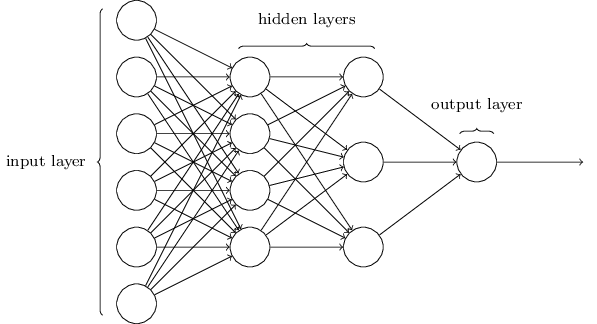
\includegraphics[width=0.25\textwidth]
    				{img/feedforward_architecture.png} 
    			}}%
    			\qquad
    			\subfloat[Convolutional Architecture]
    			{{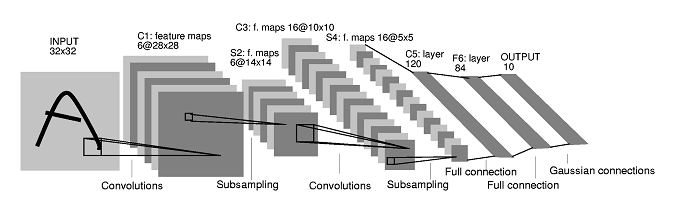
\includegraphics[width=0.45\textwidth]
    				{img/convolutional_architecture.png} 
    			}}%
    			\caption{Two of the most common architectures used for DNNs}%
    			\label{fig:architectures}
		\end{figure}		 		
		 		
		ANNs consist of a series of layers. These layers are composed of artificial `neurons' that compute a function on the inputs provided by the previous layer. They then pass the results (activations, that are typically real-valued numbers in the range [0,1]) as outputs to deeper layers. Within any individual layer there exists only one type of neuron computing the same function: these neurons are differentiated by potentially distinct inputs, outputs and weight distributions. Layers themselves are defined by the number and pattern of connections between these neurons. 
		\par 
		In order for a network to perform its task, a neural network must first be trained. This involves modifying the weights and biases of the network such that it produces the correct response for each of a number of training examples. The activations of the input units are set according to the feature values of the example, then these are propagated through the network to the output units, where the result is compared to the target output for that example and an error value calculated. This error signal is then back propagated through the network until the weights of the network have reduced the error at each node. The changes that occur are typically very small, and so large training sets are required to successfully converge the network on an optimal weight distribution. 		
		\par 
		The intuition behind back propagation, the algorithm that adjusts the weights with respect to the error value, is one of assigning 'blame'. The activations of the output nodes are determined by the activations of all the nodes below it, therefore error at the output is a result of the weights acting directly upon it from the preceding layer, and those recursively before it. In order to adjust the weights lower-down the error is backwardly propagated to the lowest hidden nodes that contributed an poor activation.			\par
		This process amounts to inductively learning how to solve a problem by exploiting regularities across a training set so that future similar examples may be classified in the same way. This is very similar to the way a human child learns, and again it's easy to see where these networks took some influence from.
\\\
\\\

\textbf{Layers}

		\par 
		There are a number of different types of layers that can be combined in a neural network: in a \textit{fully connected layer} the neurons receive an input value from every neuron in the previous layer. In a \textit{locally connected layer} the neurons are indexed spatially with inputs coming only from those nearby, and in a \textit{convolutional layer} a number of filters are applied to create a convolution. 
		\par
		The convolution of an image is produced by applying a filter upon the input image. The filter is a $k x k$ weight matrix such that $ k $ is an odd number to ensure the matrix has a true centre. The convolved image is produced pixel at a time by computing the dot product of the filter and the pixels below it, the central pixel of which is updated. A convolution is therefore produced by scanning the filter across the input pixel space until every pixel is replaced by a pixel that is some function of its filter bound neighbours. Deep successions of convolutions encode images in ways that make them invariable to translation and deformation. This is critical for classification \cite{Bruna2012}.
\par 

\textbf{Neurons}
		
		\begin{figure}[H]
    			\centering	
    			\subfloat[Multipolar Biological Neuron]												{{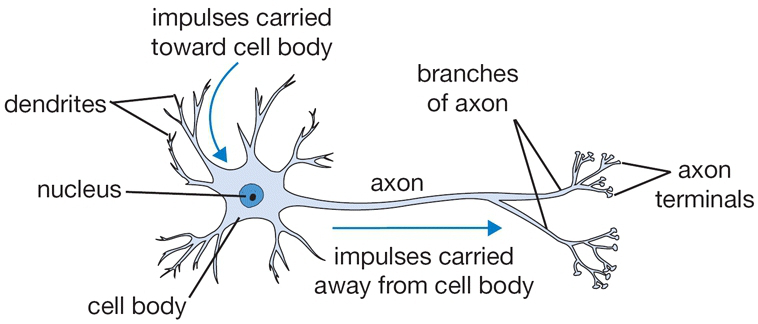
\includegraphics[width=0.25\textwidth]
    				{img/neuron_bio} 
    			}}%
    			\qquad
    			\subfloat[Artificial Neuron Model]
    			{{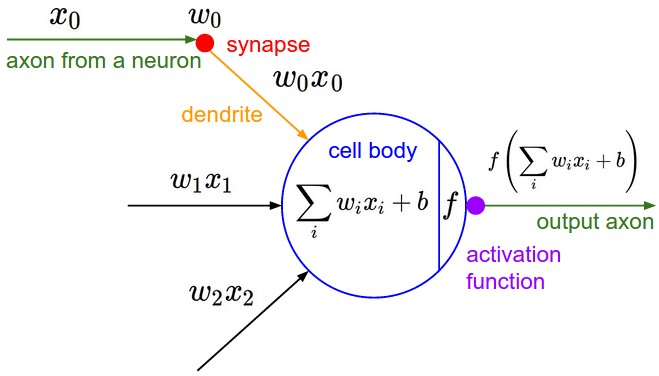
\includegraphics[width=0.25\textwidth]
    				{img/neuron_model} 
    			}}%
    			\caption{}%
    			\label{fig:biologicalNeurons}
		\end{figure}
				
		As mentioned previously, artificial neural networks are modelled on the human brain. They take influence from the \textit{multipolar biological neuron}. The neuron receives multiple electric charges from its neighbours through the dendrites. This then triggers a single electric charge to a different set of neighbouring neurons through its axon terminals. Artificial neurons perform effectively the same task and compute functions that take in multi-dimensional input but output a mono-dimensional result.
				\\\

		There are a number of different neurons used within the layers of an artificial neural network:
		\\\
		
		\textbf{Binary Threshold Neuron} 
		
		$$
		y = \begin{cases}
		1 & \text{if \textit{M} $\le \sum\limits_{i=1}^k x_{i} \cdot w_{i} + b $ where \textit{M} is a threshold parameter} \\
		0 & \text{otherwise.}
		\end{cases}
		$$

		Here, \textit{y} is the output of the neuron calculated by the weighted input acting upon it, and assessing this value against some threshold \textit{M}. The threshold neuron works much like a biological neuron in that it either outputs a charge or it doesn't. This neuron however is rarely used due to the fact that it cannot be used in optimisation algorithms, such as gradient descent, which require a function to be differentiable. 
	\\\

		\textbf{Logistic Sigmoid Neuron}	
		
		$$
		y = 
		\text{ $ \frac{1}{1 + \exp (-z)} $
		, where z = $ \sum\limits_{i=1}^k x_{i} \cdot w_{i} + b $}
		$$ 
		
		A more commonly used transfer function is the sigmoid, which is an approximation of the threshold function above. Here the bias $ b $ performs a similar function to the threshold \textit{M} in the previous example. The `threshold' can be through of as the point at which the gradient of the \textit{decision surface} is steepest. While in the threshold neuron this represents a hard boundary, the sigmoid represents a gradient of values. One disadvantage of the sigmoid is that is is more expensive to compute.
		
		\begin{figure}[H]
    			\centering	
    			\subfloat[Sigmoid A]																			{{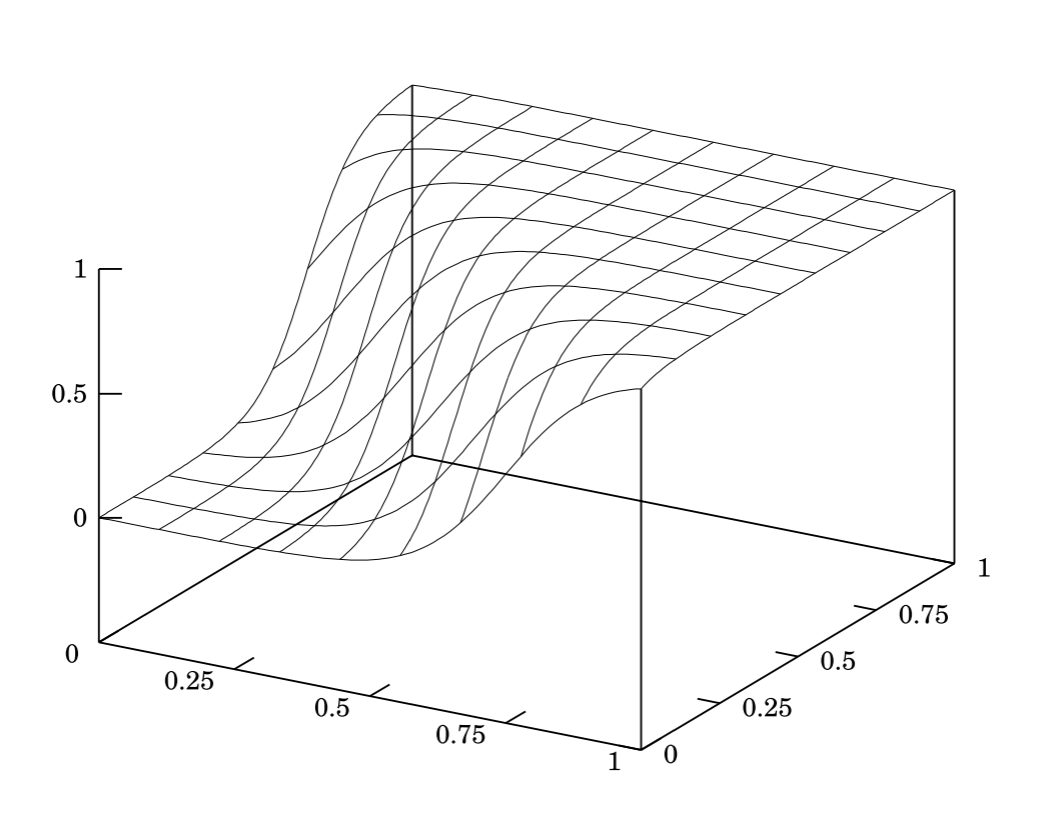
\includegraphics[width=0.2\textwidth]
    				{img/craven_sigmoid.png} 
    			}}%
    			\qquad
    			\subfloat[Threshold]																			{{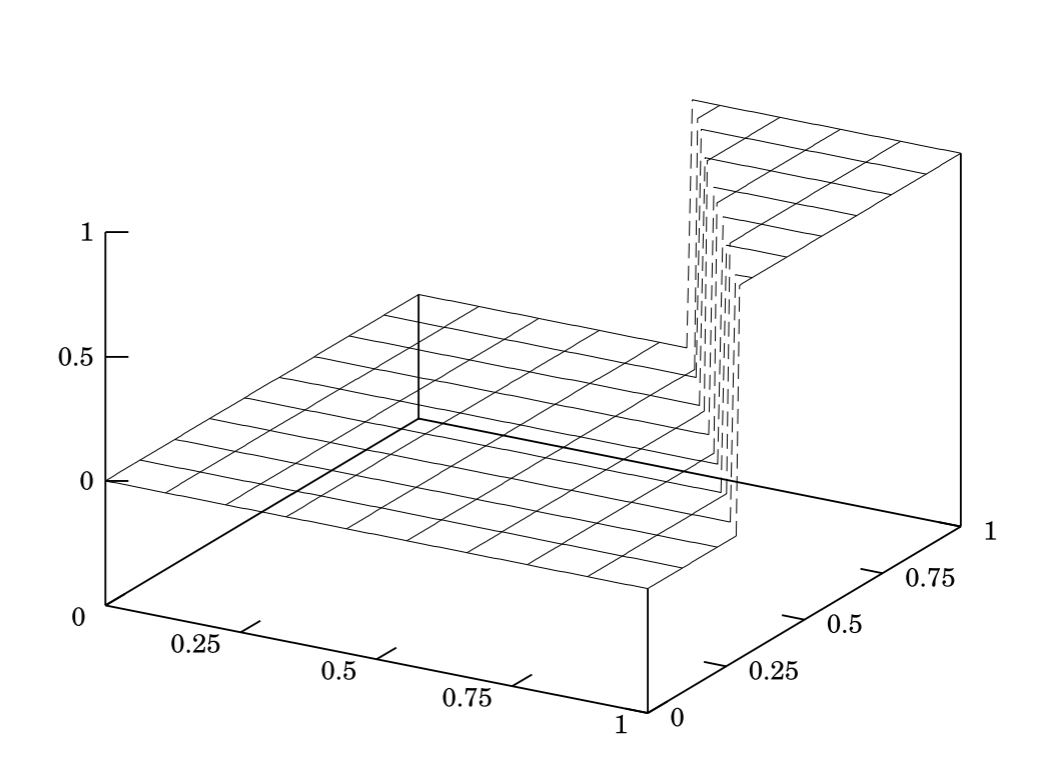
\includegraphics[width=0.2\textwidth]
    				{img/craven_threshold.png} 
    			}}%
    			\qquad
    			\subfloat[Sigmoid B]
    			{{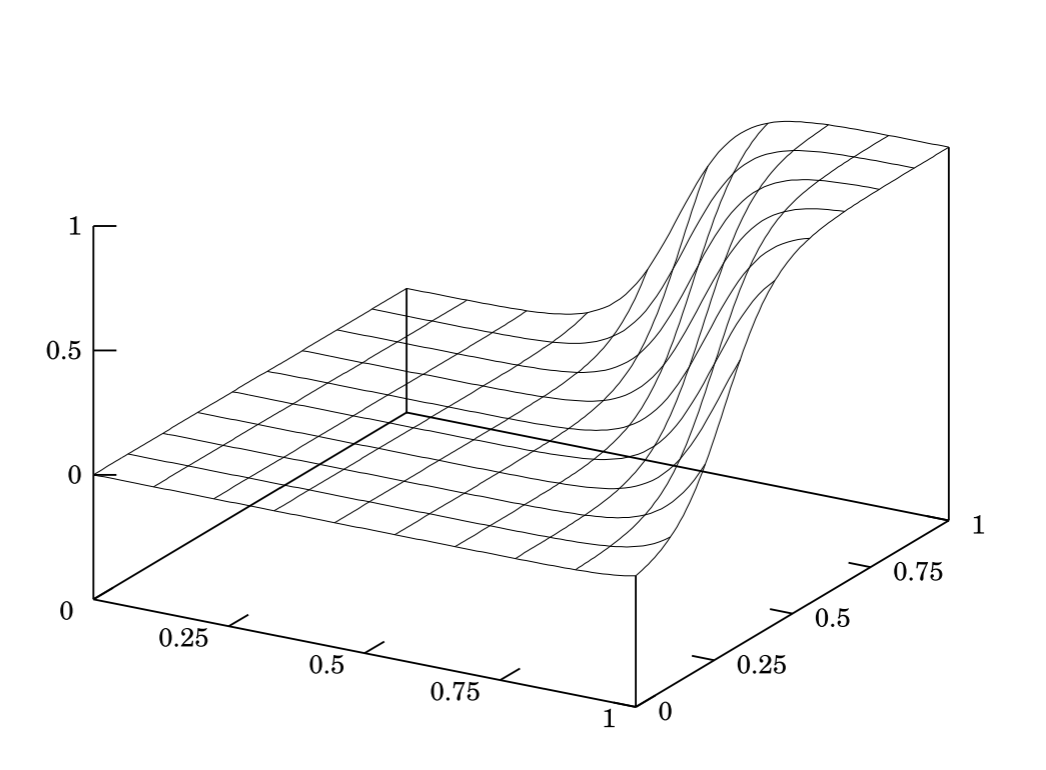
\includegraphics[width=0.2\textwidth]
    				{img/craven_sigmoid_2.png} 
    			}}%
    			\caption{}%
    			\label{fig:SigmoidNeurons}
		\end{figure}

		\textbf{Rectified Linear Neuron (ReLU) }
		
		$$
		y = 
		\text{ max$\{0,  b + \sum\limits_{i=1}^k x_{i} \cdot w_{i}\}$ }	
		$$		
		
		The rectified linear neuron is a hybrid function. It is more efficient to compute that the sigmoid neuron and is partially differentiable, thus making it suitable for gradient descent. The compromise here is the cost of sophistication of the result. The neuron introduces a non-linearity with its angular point, a smooth approximation of which is the softplus $f(x) = log(1 + e^{x}))$.
		
\textbf{Architecture}
		The standard deep neural network architecture is the feedforward network (FFNN) explained more fully previously. Variations exist; however such as recurrent neural networks (RNNs), convolutional neural networks (CNNs) and a few others. 
				
\textbf{Convolutional Neural Networks:}
		are typically used for image classification due to their ability to successfully capture \textit{local} structure. The first layers are convolutional and produce a featurized representation of an image such as those that emphasize edges or compute gradients of hue and value. Successive layers are more standard and undergo a smiliar non-linear transformation. The output is usually a vector of probabilities spread across different possible classifications.
		\\\
		\textbf{Design Space}
		In a typical machine learning workflow, including working with ANNs, practitioners iteratively develop algorithms by refining choices in areas such as feature selection, sub-algorithm selection, parameter tuning and more \cite{Patel2008}. This is usually done through a trial and error approach that is perhaps similar to hill-climbing in the model space. This is highly unscientific, with only a few outputs providing direction such as error.
		\par 
		The most challenging and time-consuming part of training a neural network lies in selecting the correct parameters, of which there are many, and each affects the network in an almost unknown capacity. Some examples are:
				
		\begin{figure}[H]
    			\centering	
			{{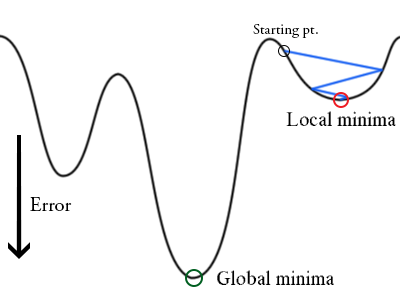
\includegraphics[width=0.3\textwidth]
    				{img/gradient_descent.png} 
    			}}%
    			\caption{Gradient Descent}%
    			\label{fig:GradDesc}
		\end{figure}		
		 		
		\par
		\textbf{Size of Filters:} if the filter is too small features will be too coarse, however if the filter is too large the complexity of a model increases significantly with little benefit.
		\par
		\textbf{Number of Layers:} additional layers tend to improve performance, however they also increase a models complexity and thus its training time - this means that fewer model iterations are possible with a set time period. Back propagation issues with layers failing to train, can also arise.
		\par 
		\textbf{Filters per Layer:} additional filters likewise tend to improve performance, and again there is likely to be a cut-off point where diminishing returns are outweighed by increased model complexity and training time.
		\par  
		\textbf{Layer Connectivity:} variations in locally-connected and fully-connected layers can change performance dramatically, such as exhibited in the difference between convolutional layers, connected layers and those with dropout.
		\par 
		\textbf{Input and Output Data Encodings:} different vector encodings change the way the network learns. Images for example with a height, width and three colours per pixel are compressed into a one-dimensional vector as an effective input encoding.
		\par  		
		\textbf{Error Space, or Bound:} changes how the network perceives error, and thus fundamentally effects what it learns during the backpropogation optimisation period.
		\par
		
		\begin{figure}[H]
    			\centering	
			{{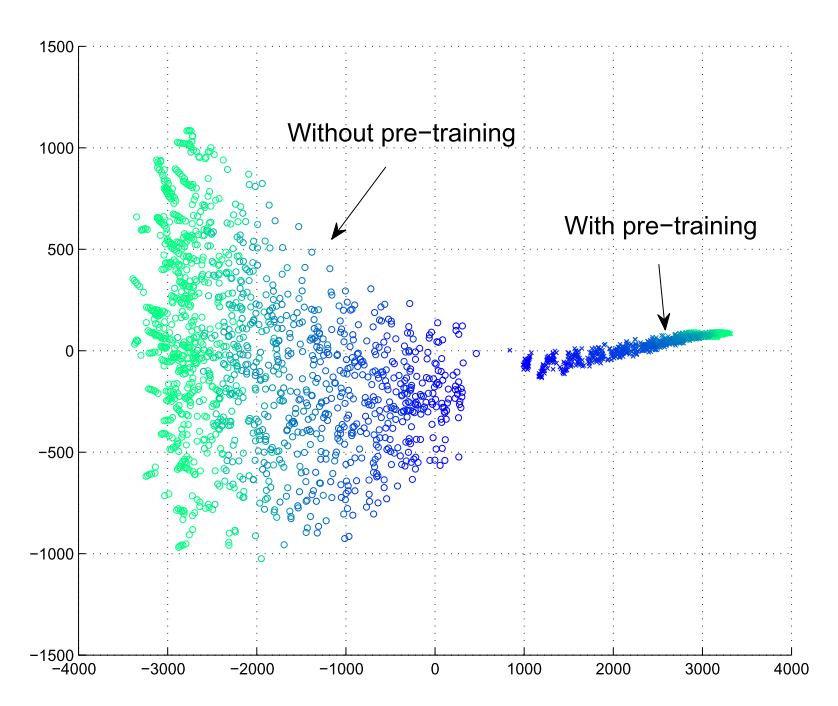
\includegraphics[width=0.3\textwidth]
    				{img/erhan_pretraining_versus.png} 
    			}}%
    			\caption{Error plot with and without pretraining}%
    			\label{fig:Error}
		\end{figure}	
		 		
		\textbf{Initialization of Weights:} can also alter how a model learns. There are a number of different possible approaches to this: such as uniformly, randomly, as a gaussian, unsupervised pre-training and more.
		
		\par 
		\textbf{Auxiliary Layers:} in ConvNets for example, pooling and normalization layers are often applied, however each has it's own set of additional parameters to tweak and a different effect on the model, thus requires complex tuning.
		\par 
		\textbf{Non-linear functions:} can make a large difference on model performance: the choice of which non-linearity you choose, for example choosing a 'Rectified Linear' neuron as opposed to a 'sigmoid'. 
		\par 
		\textbf{Optimization Parameters:} such as step-size, or learning rate, regularisation, mini-batch sampling all need to be tuned for maximum accuracy and convergence speed. While there are common algorithms that help choose these parameters, such as AgaGrad \cite{Duchi2011}, manual tuning is often still required, and is difficult to get right.
		\par
		\textbf{Momentum Co-efficient:} adds a fraction of the previous weight update to the current one, and is used to prevent the system from converging to a local minimum or saddle point, and increase the speed at which it converges. Too high and risk of overshooting the minimum, and too low the system might still hit a local minima.
		\par
		
		\begin{figure}[H]
    			\centering	
    			\subfloat[Without Dropout]							{{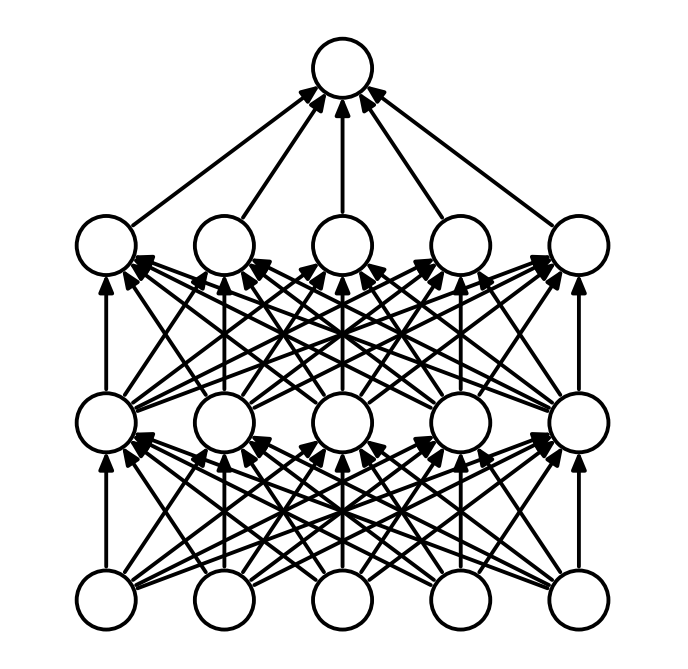
\includegraphics[width=0.25\textwidth]
    				{img/without_dropout.png} 
    			}}%
    			\qquad
    			\subfloat[With Dropout]
    			{{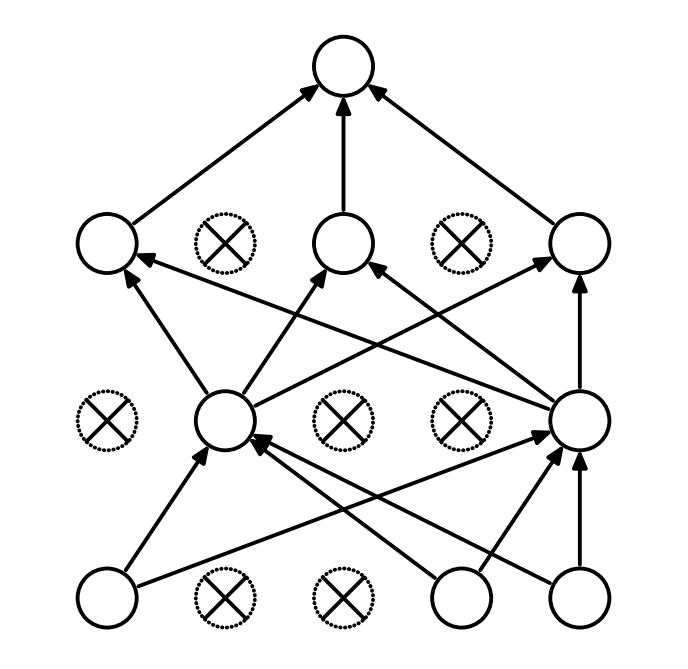
\includegraphics[width=0.25\textwidth]
    				{img/with_dropout.png} 
    			}}%
    			\caption{}%
    			\label{fig:Dropout}
		\end{figure}
		
\textbf{Problem}	
		While there have been a number of improvements to neural networks over the years, such as the development of dropout, they remain to be considered as black box, especially in comparison to some other better studied and less complex machine learning techniques such as support vector machines or logistic regression. There is still no clear understanding of why they perform so well or why certain combinations of internal weights and connections enable highly complex tasks, such as computer vision, to be performed. It is as result of this lack of understanding that the development of new models falls largely upon a `greedy' trail and error approach. This is unsatisfactorily unscientific, using experience and intuition as the primary guiding factors.
		\par
		There are a number of challenges that arise in attempting to change this way of working; firstly, these networks are composed of many functional components, the values of which as individuals and as a whole are not readily understood. In addition, each component of a network may have dozens of hyper-parameters linked to it, every one of which needs to be tuned to attain optimal performance. Finally, exacerbating these issues is that literature hasn't formalised methods for development or discussion, so even experts can only rely on others anecdotal results to guide design.
		\par 
		In real terms, this means that designing and debugging deep neural networks is error-prone and time-intensive. 
		\par 
		It is hoped that alternative work flows may provide some deeper insight. \cite{Jarrett2009} for example uses a number of pre-evaluated models compared against number of datasets to make more informed decisions, this however doesn't leave room for new discovery. \cite{Bergstra2013} uses a less human involved approach by using Bayesian statistics to automate the search of the parameter space, this is however computationally demanding and doesn't always provide an optimal solution. Another area is to support decision making with visualisation allowing for the constant evaluation of clear representations to help researchers better understand the trajectory they are taking their models in as they go through the standard trail and of error tweaking different parameters.
		\par
		Visualisation is not uncommon, and similar projects have been undertaken across a variety of areas within Machine Learning, in the visualisations of the naive-Bayesian network \cite{Becker2001}, decision trees \cite{Ankerst1999}, Support Vector Machines \cite{Caragea2001} and Hidden Markov Models \cite{Dai2008}. Studies have shown that integrating such tools into the learning work flow can in fact produce better results than automated techniques alone \cite{Ware2002}.

\subsection{Visualisation}

%\subsubsection{Overview}
\textbf{Overview}

		Visualising quantitative information typically involves displaying measured quantities, or data, by means of the combined use of points, lines, a coordinate system, numbers, symbols, words, shading, and colour. These visual forms are more rapidly understood and are easier to critique than the information underlying them \cite{DeFanti1989}, \cite{McCormick1987}, \cite{Tufte2001}.
		\par
		In a numerical format vast quantities of data can be tedious to process, and often little can be gleaned from such complex models. Visual data on the other hand communicates to the highly developed visual pattern-recognition capabilities of humans. A majority of our brain's activity deals with the processing and analysis visual images. Images are pre-attentive and processed before text. Several empirical studies show that visual representations are superior to verbal or sequential representations across a number of different tasks; illustrate relations, identify patterns, to present overview and details, to support problem solving and to communicate different knowledge types \cite{Burkhard2004}. As a species we are far better at recognising regularities, anomalies, and trends in images rather than in long lists of numbers \cite{Ware2010}. Consider how difficult is may be to observe both global and local patterns in a list of numbers, than across some standard visualisation such as a graph.
		\par 
		For data mining to be effective, it is important to include the human in the data exploration process and combine the flexibility, creativity and general knowledge of the human with the enormous storage capacity and computation power of computers. Visual data mining techniques have proven to be of high value in exploratory data analysis and they have high potential for exploring large datasets. Visual data exploration is especially useful when little is known about the data and the exploration goals are vague. Since the user is directly involved in the exploration process, shifting and adjusting the exploration goals can be automatically done if necessary \cite{Keim2002}.
		\par 
		The canonical example of the usefulness of visualisation lies in the Anscombes quartet, where the four sets of numbers in the quartet have many identical summary statistics - mean of x values, mean of y values, variances, correlations and regression lines - but vary wildly when graphed \cite{Shoresh2011}:

		\begin{figure}[H]
    			\centering	
				{{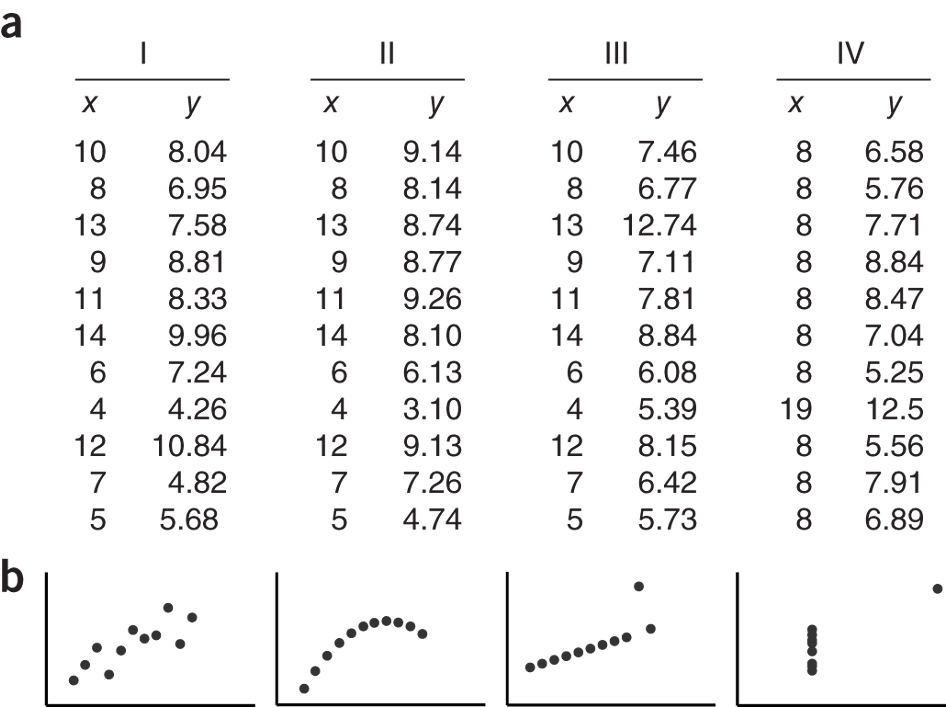
\includegraphics[width=0.5\textwidth]
    				{img/anscombes_quartet} 
    			}}%
    			\caption{(a) The four sets of numbers that form Anscombe's quartet -  (b) The highly distinctive graphs that result from plotting the data in a.}%
		\end{figure}
		
		\par 
		Your message should be represented clearly by taking advantage of the strengths of visual perception, while avoiding all its weakness. At the same time, the representation should match the human thought process, augmenting where necessary to cover up limitations \cite{Tufte2012}.
		\par 
		
%\subsubsection{Tufte: what makes a good visualisation}
\textbf{Tufte: what makes a good visualisation}
		
		Edward Tufte, a founding figure in laying out the core principles of data visualisation, provides us with a set of basic commandments \cite{Tufte2001}:
		
		\begin{itemize}
			\item show the data
			\item induce the viewer to think about the substance rather than about methodology, graphic design, the technology of graphic production, or something else
			\item avoid distorting what the data has to say
			\item present many numbers in a small space
			\item make large data sets coherent
			\item encourage the eye to compare different pieces of data
			\item reveal the data at several levels of detail, from a broad overview to the fine structure
			\item serve a reasonable clear purpose: description, exploration, tabulation or decoration
			\item be closely integrated with the statistical and verbal descriptions of a data set
		\end{itemize}

		Tufte additionally provides a set of rules regarding graphical excellence:
		
		\begin{itemize}
			\item create a well-designed presentation of interesting data - a matter of \textit{substance}, of \textit{statistics}, and of \textit{design}
			\item ensure that complex ideas are communicated with clarity, precisions, and efficiency
			\item give to the viewer the greatest number of ideas in the shortest time, with the least ink, in the smallest space
			\item convey multivatiate data
			\item tell the truth about the data
		\end{itemize}
		 
		\begin{figure}[H]
    			\centering	
			{{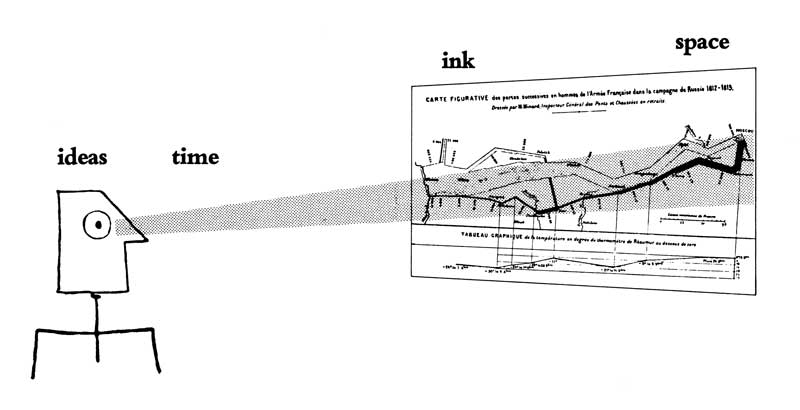
\includegraphics[width=10cm]
    				{img/graphical_excellence} 
    			}}%
    			\caption{Tufte's illustration of graphical excellence}%
    		\label{fig:TufteExcellence}
		\end{figure}

		\par 
		 
		A final set of Tufte \cite{Tufte2001} principles:
		\par
		\textbf{Principle One:} \textit{show only as much as is required}
		\par 
		This is Tufte's \textit{data-ink} principle - irrelevant content is distracting, so should be removed. It is common place today to find charts and graphs with all sorts of 3D effects, unwanted background images and colours. The idea of having a data-ink ratio is to show only as much information as is required.
		$$
		\text{Data-ink ratio} = 
		\frac{\text{data-ink}}{\text{total ink used to print the graphic}}
		$$
		\\\
		\textbf{Principle two:} \textit{include visual differences only when required} 
		\par
		The human brain has an amazing capability of spotting visual differences such as color, size and position. Often they look for the meaning to change depending on how these visual features and designed. If there is no difference, but embellishments are added, it often leads to confusion.
		\\\ 
		\textbf{Principle tree:} \textit{use visual encodings for quantitative values}
		\par 
		Successful examples are: length, for example the length of bar in a bar graph; 2-D location, for example the position of a data point in a scatter plot; size, for example the area in a pie chart; shape, orientation or hue, for example denoting different classes in any graph. All of these are automatically and immediate understood as they have natural properties that humans understand. 
		\\\
		\textbf{Principle four:} \textit{differences in visual properties should correspond to actual differences the data}
		\par 
		Its important to encode differences consistently and not manipulate the visualisation to aid an argument. For example, ensuring that axes are consistent - from zero to some useful value without undergoing any form of distortion.
		\\\
		\textbf{Principle five:} \textit{do not visually connect values that are discrete}
		\par 
		In a graph, when you draw lines between discrete values and connect them, people perceive those values as having a relationship to each other, and so this should be avoided.
		\\\
		\textbf{Principle six:} \textit{visually highlight the most important part of your message}
		\par 
		All information on a chart might not be equal and it might be possible to direct a users attention to a particular part of the visualization by visually highlighting through use of color, position or another standard encoding.
		\\\
		\textbf{Principle seven:} \textit{augment short term memory through visual patterns}
		\par 
		The human brain is limited to retaining around four pieces of information at any given time. By presenting quantitative information as visual patterns, more information can be simultaneously stored as one `piece'.
		
		\begin{figure}[H]
    			\centering	
    			\subfloat[Poor Line Weights: unclear]												{{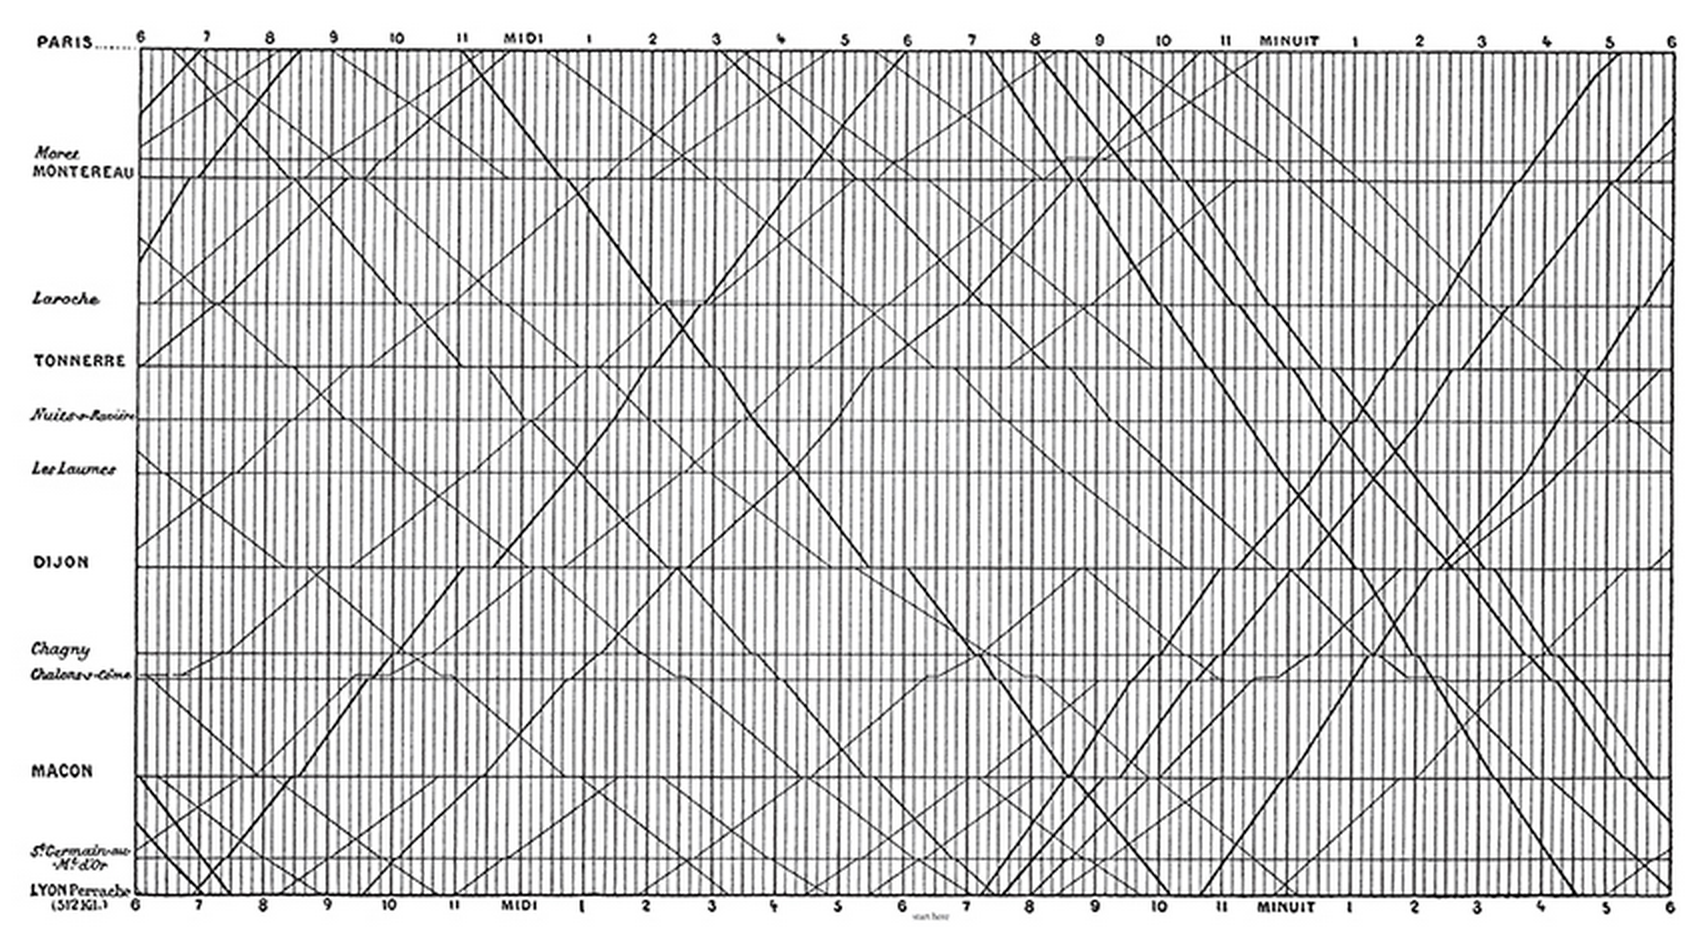
\includegraphics[width=7cm]
    				{img/marey_train_bad.png} 
    			}}%
    			\qquad
    			\subfloat[Better Line Weights: clear]
    			{{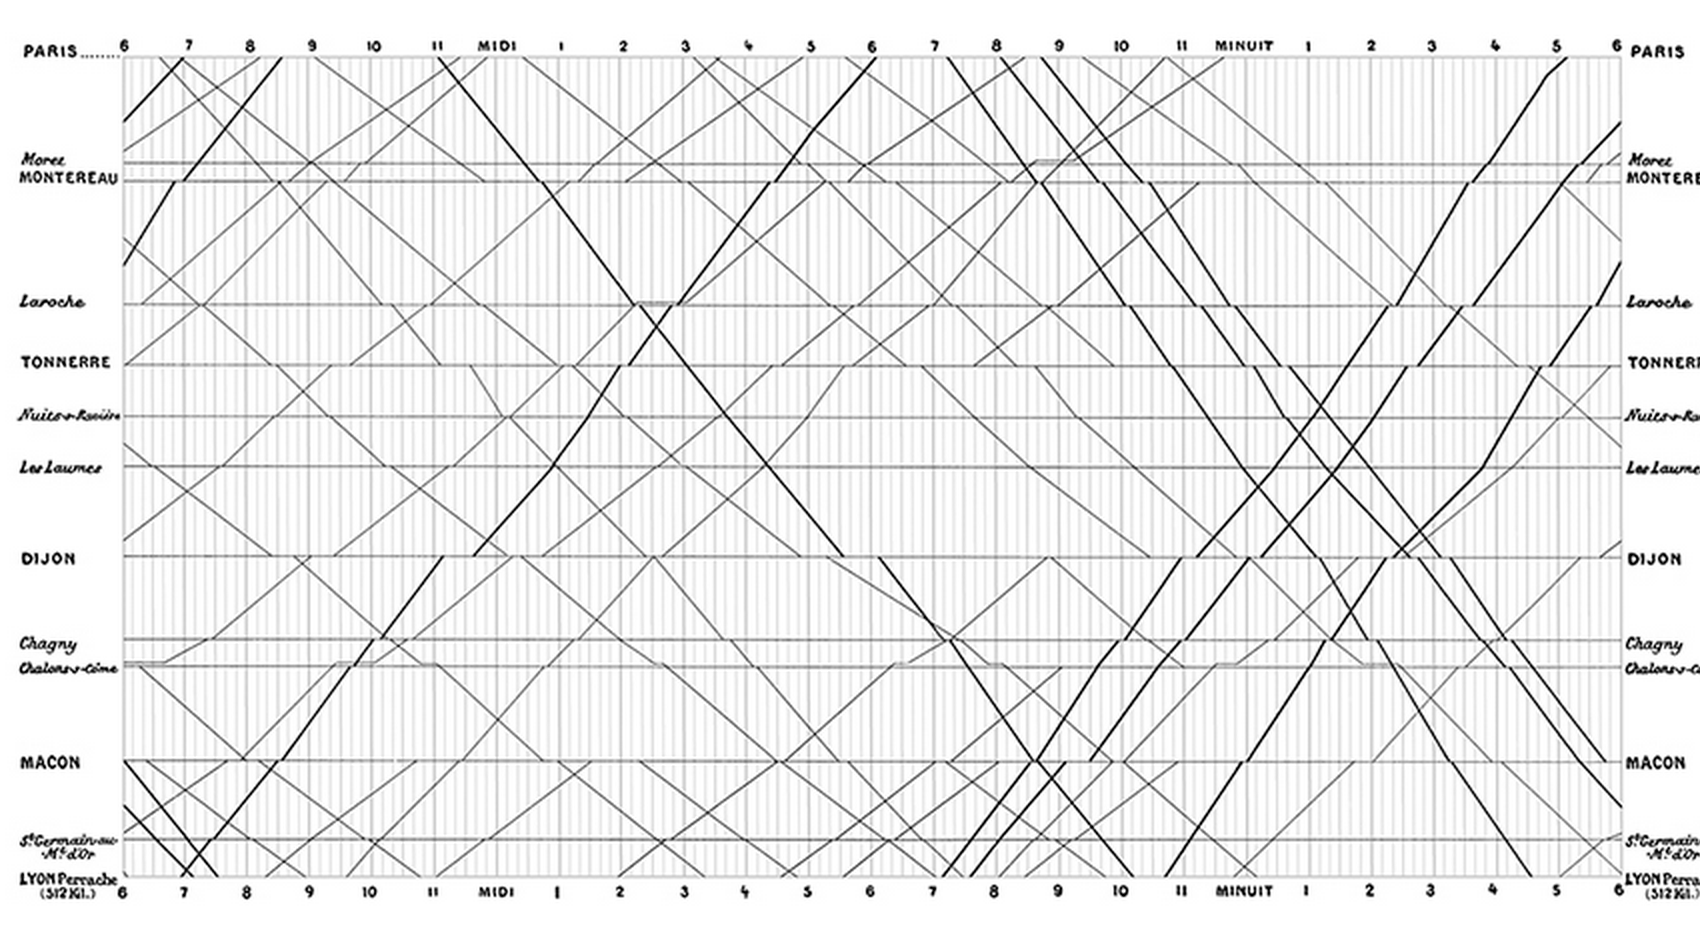
\includegraphics[width=7cm]
    				{img/marey_train_better.png} 
    			}}%
    			\caption{Tufte's train line chart demonstrating excessive data-ink}%
		\end{figure}
	
			
\textbf{Active Vision}
		
		\begin{figure}[H]
    			\centering	
			{{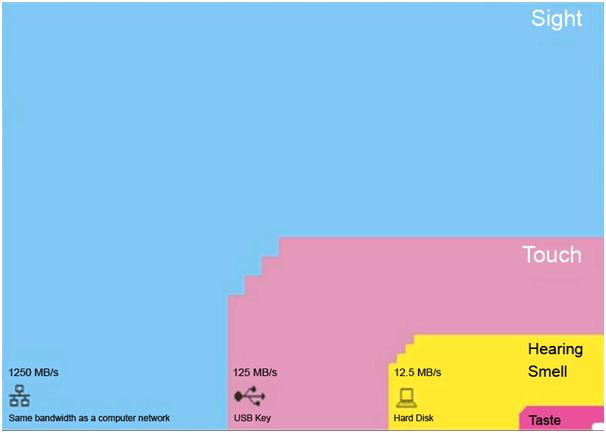
\includegraphics[width=0.3\textwidth]
    				{img/brain_bandwidth.png} 
    			}}%
    			\caption{Tor Nørretranders Brain Bandwidth}%
    		\label{fig:TufteExcellence}
		\end{figure}
		

 		There has been a small revolution in our understanding of human perception, sometimes called `active vision' \cite{Ware2010}. Active vision means that we should think about graphic designs as more than pretty images, but as cognitive tools that enhance and extend our brains. Diagrams, maps, web pages, information graphics, visual instructions, and more regularly help us to solve problems through a process of visual thinking, using the enormous proportion - almost half - of the human brain that is devoted to the visual sense.  
	
		\par 
		Danish Physicist Tor Nørretranders discusses the ``bandwidth of our senses ” in computer terminology to give an idea of the power of this visual system. In the diagram it's amusing to observe the comparison, especially to the small white box at the corner which is \textit{0.7\%} of total power and is what we are aware off when all this processing is happening \cite{Tufte2012}.		
		\par 
		\textit{``We are all cognitive cyborgs in this Internet age in the sense that we rely heavily on cognitive tools to amplify our mental abilities. Visual thinking tools are especially important because they harness the visual pattern finding part of the brain."} \cite{Ware2010}.
		\par 

%\subsubsection{Visual Problem Solving}
\textbf{Visual Problem Solving}
	  		 
  		\begin{figure}[H]
    			\centering	
			{{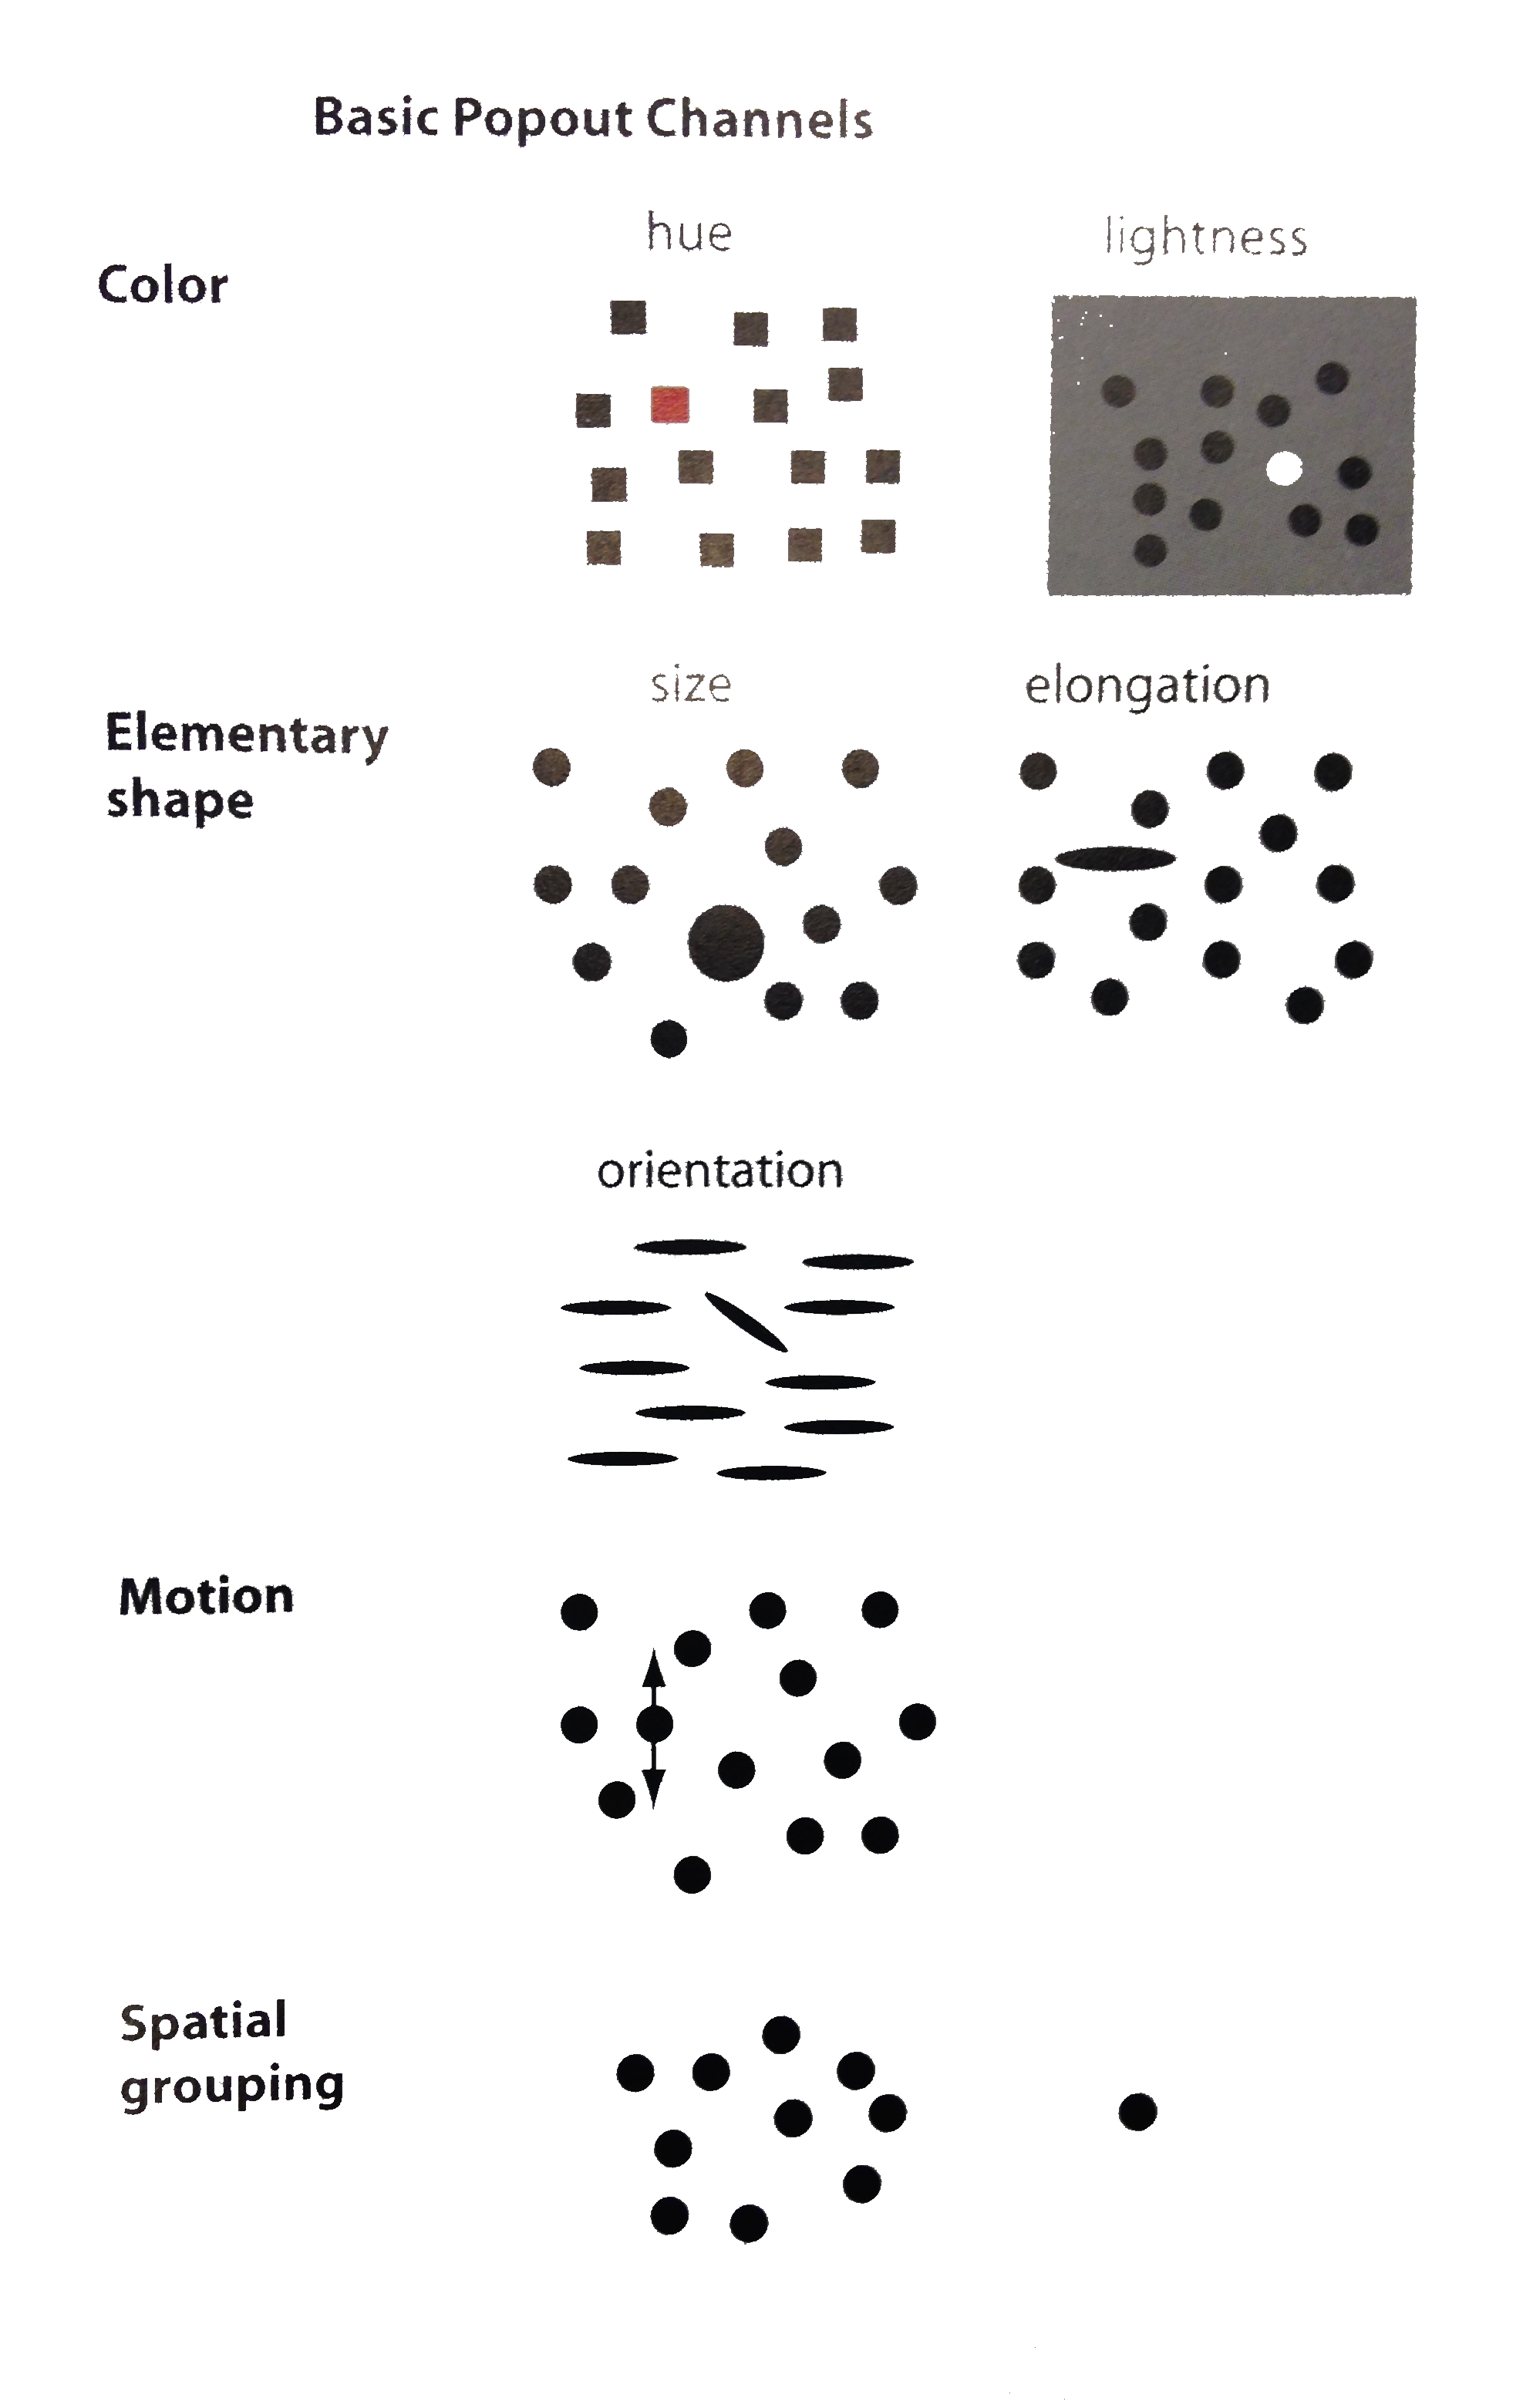
\includegraphics[width=0.3\textwidth]
    				{img/ware_popout_channels.png} 
    			}}%
    			\caption{Ware's things that pop-out}%
    		\label{fig:Ware Pop-Out}
		\end{figure}
  		 
		A useful way to describe the way the brain operates when it solves problems is as a set of nested loops \cite{Ware2010}. Outer loops deal with generalities, inner loops process the details. 
		\par 
		\textbf{Overview:} an outerloop constructs a series of steps to solve the problem and then executes them. For example, when observing the London Underground Map, these problems might be `find end point stations' or `find intersections' etcetera.
		\par 
		\textbf{Filter:} a middle loop will perform a visual search in order to find patterns that address the query above. This involves a series of rapid eye movements. 
		\par 
		\textbf{Details:} The inner loop will be activated when the eye arrives at a point of fixation: and the process of visual testing begins and patterns are evaluated at a rate of about twenty per second. 
		\par 
		When producing data visualisations it is important to think about the particular details of design. What does it take to make a graphic symbol that can be found rapidly? How can something be highlighted? The problem for the designer is to ensure all visual queries can be effectively and rapidly served \cite{Keim2002}. 

		\subsubsection{Visual Properties}
  		 
  		 Human brains and visual systems have evolved to be highly sensitive to specific types of visual stimuli. The brain interprets stimuli in different ways and with varying levels of accuracy. For example, human brains can accurately differentiate between many different sizes, but only a relatively small number of line weights. The perceived area of a circle in fact grows more slowly than the actual physical and measured area. Experiments \cite{Meihoefer1973} show in fact that \textit{perceived area = $(actual area)^{x}$, where} $ x= 0.8 \pm 0.3 $. Human brains naturally consider lengths to be ranked, but not patterns. Some arrangements of lines imply groundings, whereas others imply hierarchies. Knowing how to use these properties effectively has a powerful effect on the accessibility and utility of a visualisation.\cite{Iliinsky2013}
		\\\
		There are a number of basic data types that can be visually encoded in some ways better than others:
		\par 
		\textbf{Categorical} groupings of things that are alike, but not ranked, ordered or numbered; flavours, regions, teams and other collections. 
		\par 
		\textbf{Quantitative or numeric} a numeric measure; dollars, units shipped, population and distance. 
		\par 
		\textbf{Ordinal} data that is ordered or ranked, and the sequence matters, but there isn't necessarily a specific value; steps in processes or sequences of events. 
		\par 
		\textbf{Relationship} includes grouping, hierarchy, influence, correlation or other non-numeric interactions; military rank, lists of requirements, etcetera. 
		\par 
		The visual properties most compatible with the above datatypes are determined by two fundamental factors: the number of useful variations or values of that visual property that the brain can perceive and whether or not the brain interprets that visual property as naturally ordered. 
				
		\begin{figure}[H]
    			\centering	
			{{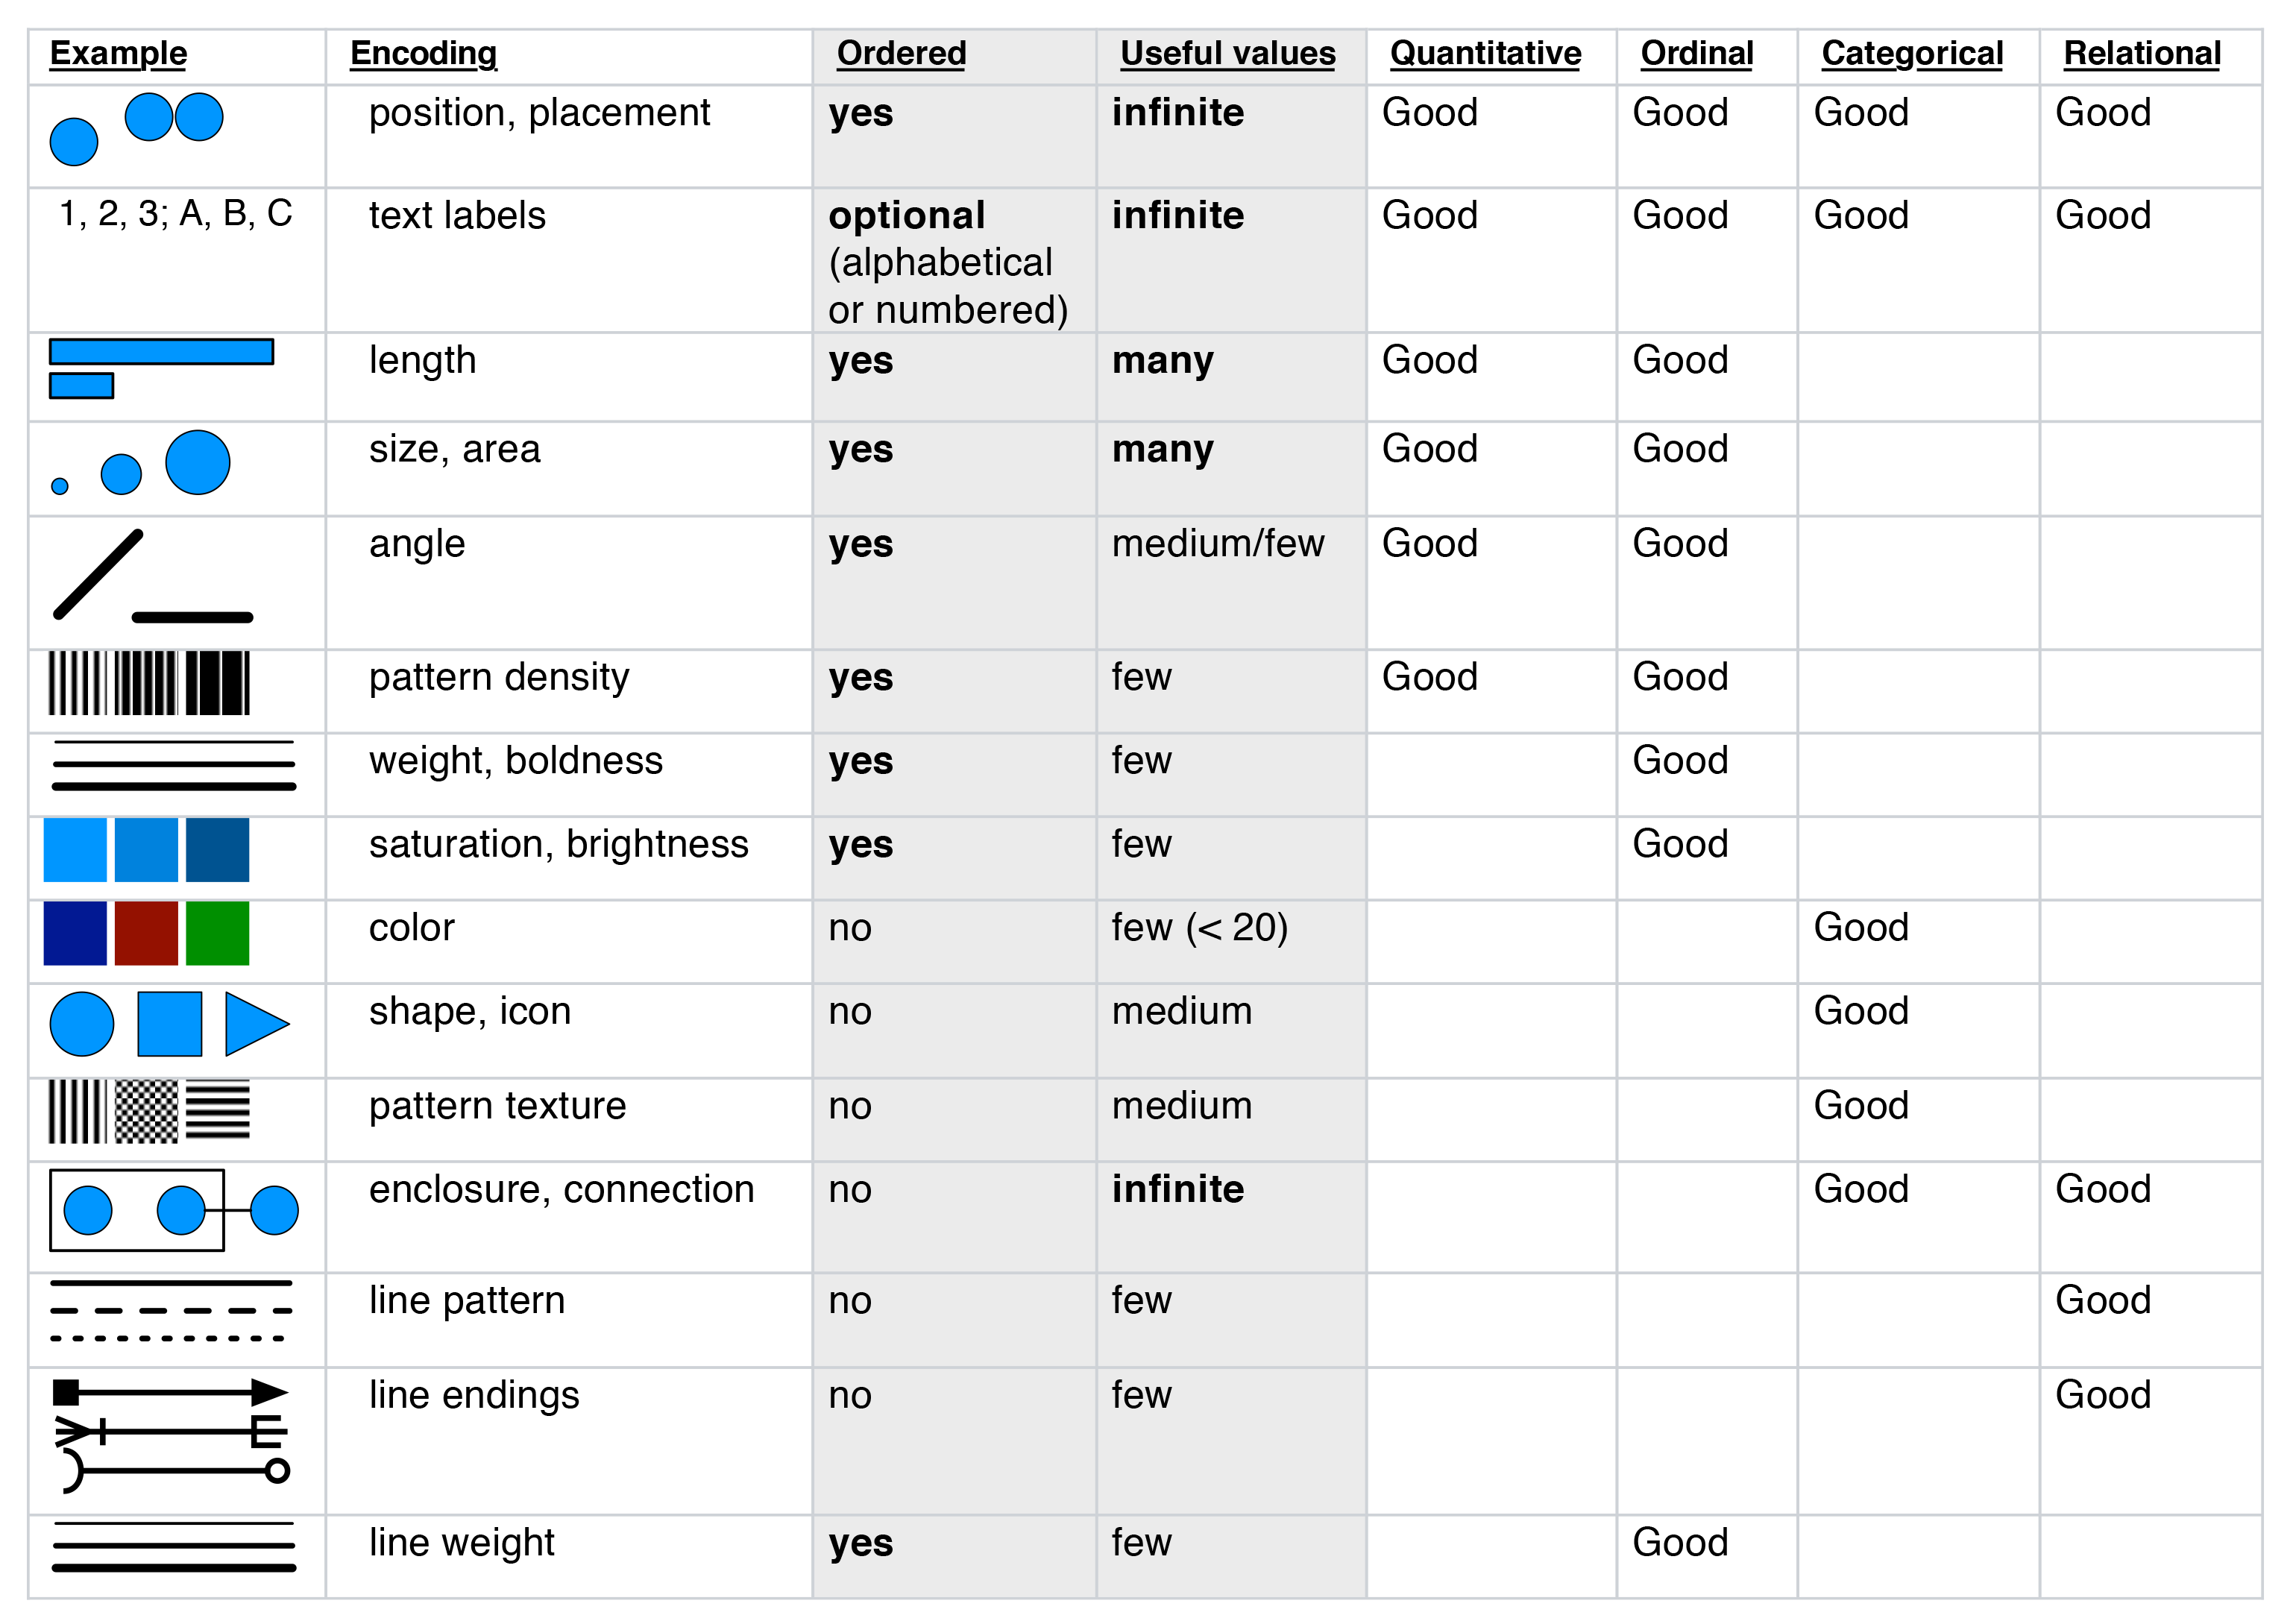
\includegraphics[width=10cm]
    				{img/noah_illinsky_visual_encodings.png} 
    			}}%
    			\caption{Illinky's rules for 2D graphical encodings}%
    			\label{fig:illinsky}
		\end{figure}
		
		\par 

	\subsubsection{Some standard visualisation types}

	\begin{figure}[H]
    			\centering	
			{{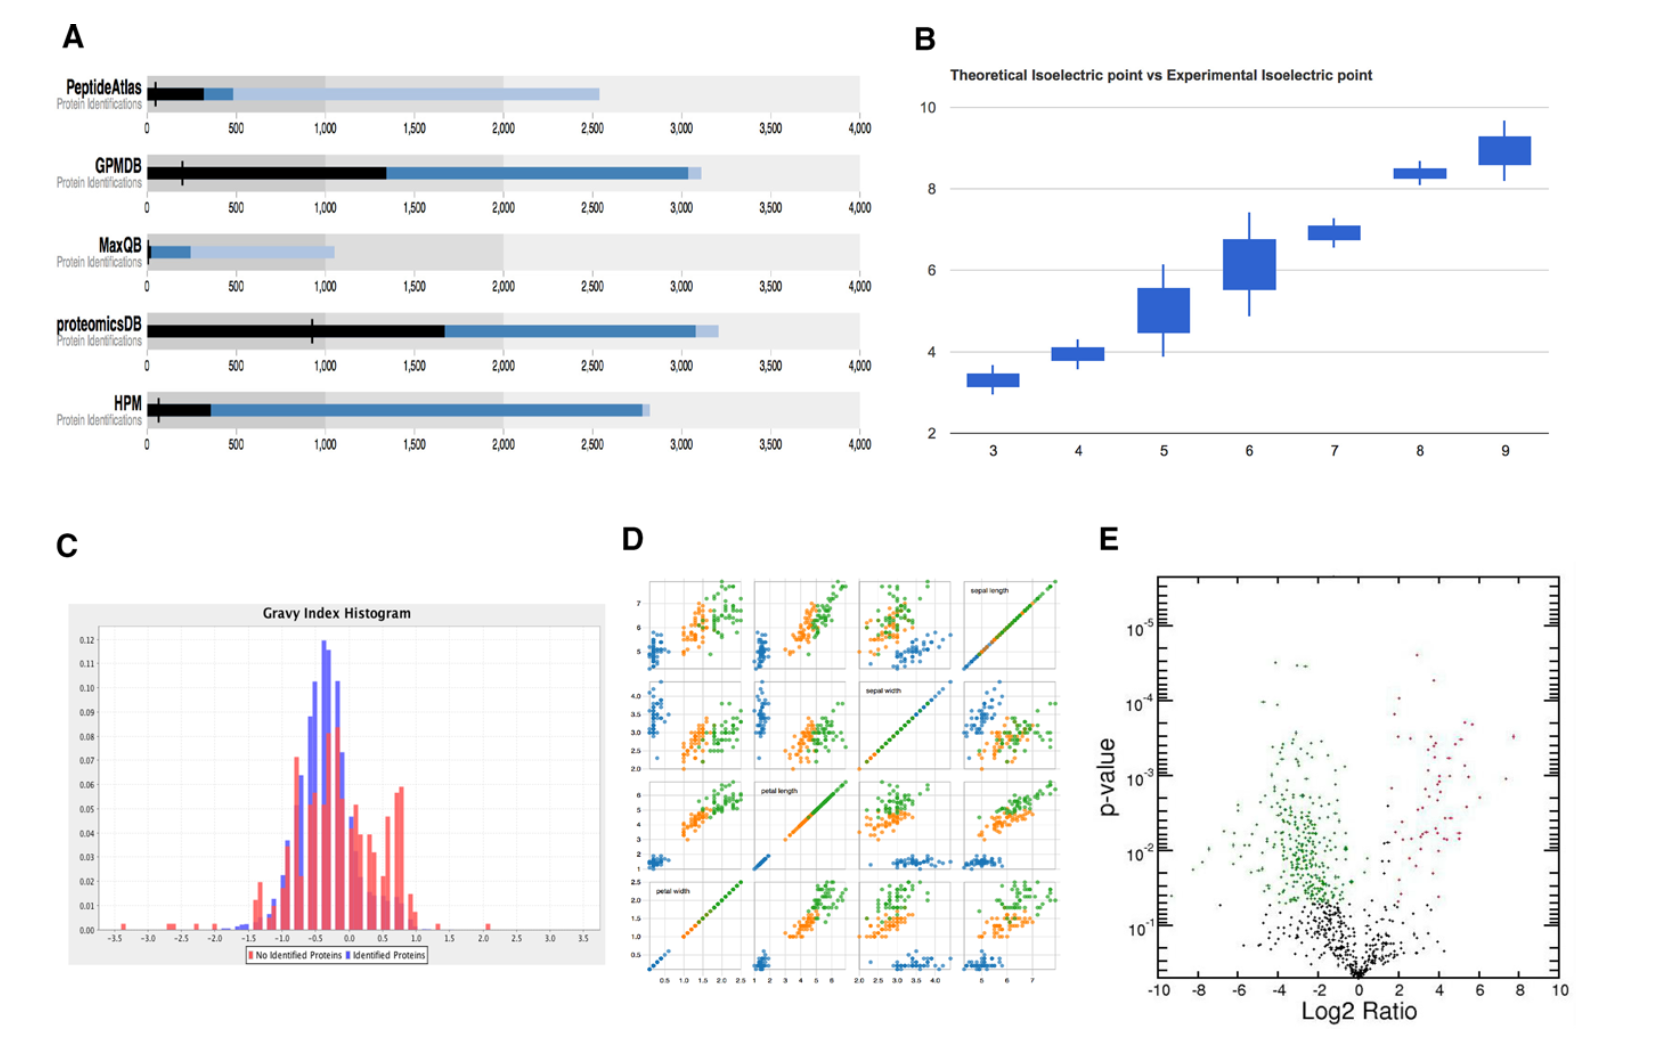
\includegraphics[width=10cm]
    				{img/rui_wang_charts.png} 
    			}}%
    			\caption{Charts}%
    		\label{fig:illinsky}
	\end{figure}

 		
		\textbf{Charts:} Charts are probably the most popular techniques; they are very effective in presenting two or three dimensional data. There are many types of charts: x-y (and -z) plots, line graphs, bar and column charts, area charts, stacked bars and column graphs, histograms, pie charts, doughnut charts, box plots and many more \cite{Wang2015}. 

	\begin{figure}[H]
    			\centering	
			{{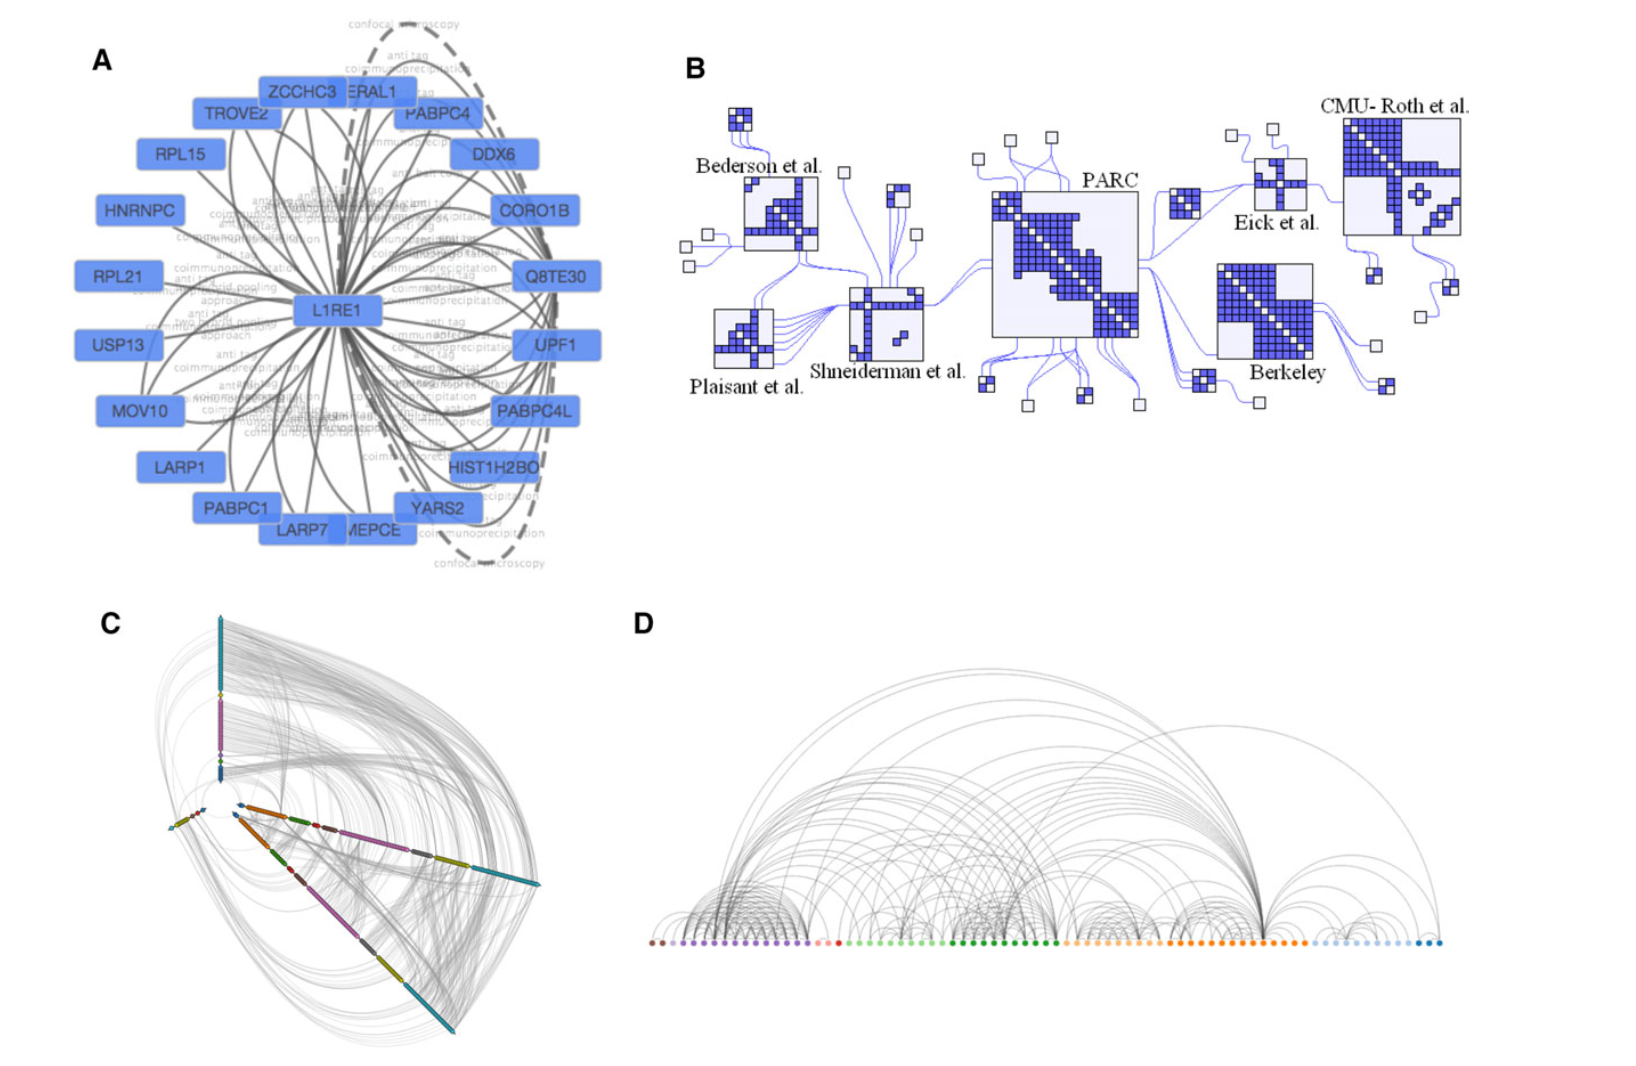
\includegraphics[width=10cm]
    				{img/rui_wang_networks.png} 
    			}}%
    			\caption{Networks}%
    		\label{fig:illinsky}
	\end{figure}
	
		\textbf{Networks:} Node-link diagrams represent a powerful way of understanding entity relationships by showing their overall structure and the topology of the network. Node-link diagrams have the advantage of preserving local relationships. They make it easier to identify the nearest neighbours for example of a particular node or find the shortest path between two nodes.
	
	\begin{figure}[H]
    			\centering	
			{{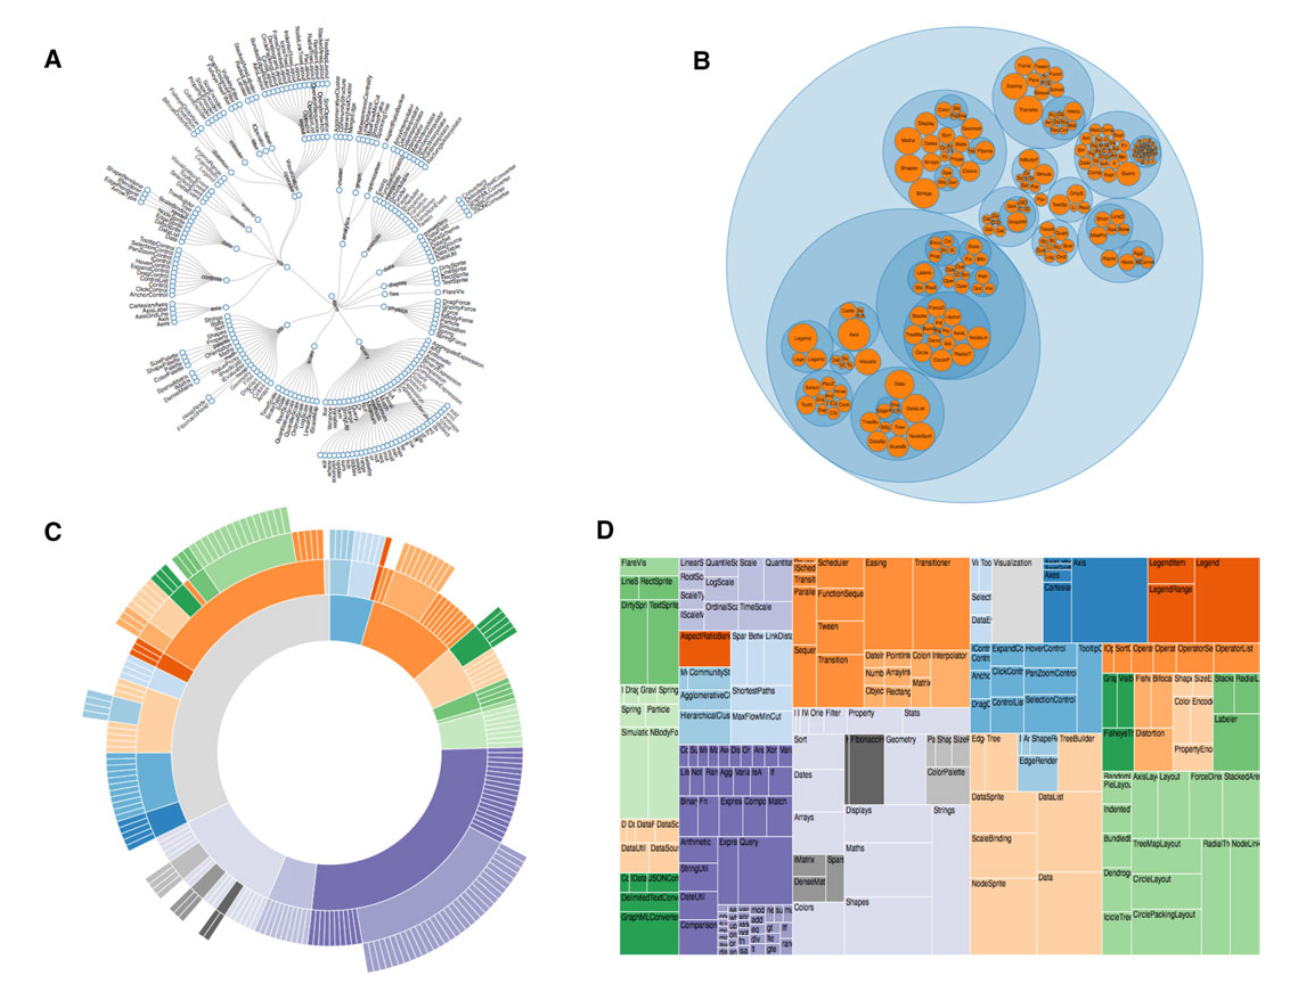
\includegraphics[width=10cm]
    				{img/rui_wang_hierarchies.png} 
    			}}%
    			\caption{Hierarchies}%
    		\label{fig:illinsky}
	\end{figure}

		\textbf{Hierarchies:} Common reasons to use hierarchies are, among others, are to gain insight to the structure of the hierarchy, to understand the distribution of data within the context of the structure, or to provide a summary of the data set into aggregated data in order to avoid information overload.
		
		\subsubsection{New Visual Encodings for Deep 	Learning}
 			
	\begin{figure}[H]
    			\centering	
			{{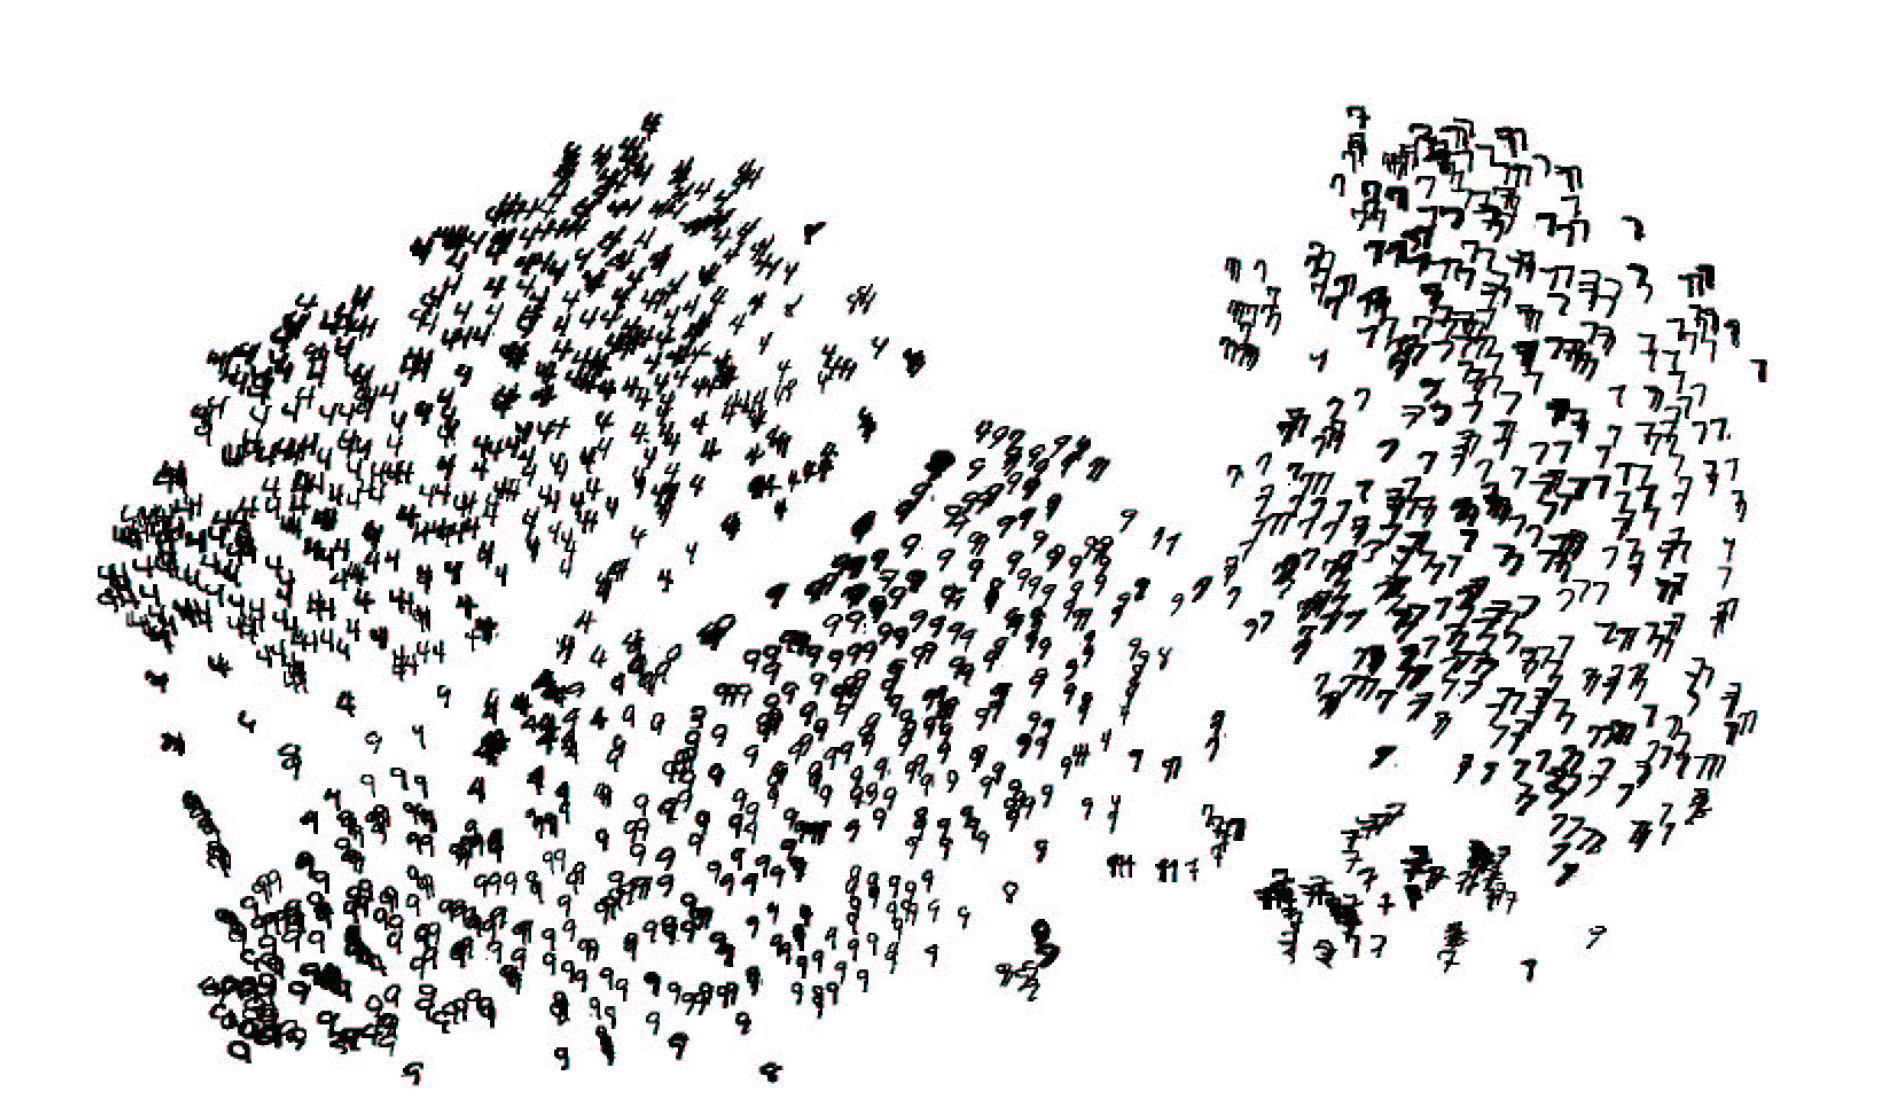
\includegraphics[width=0.3\textwidth]
    				{img/hinton_embedded_tsne.png} 
    			}}%
    			\caption{MNIST embedded digit plot}%
    		\label{fig:mnistHinton}
	\end{figure}
 		

		While there are a number of established best practices for visualising low dimensional data as explored above, many of these simply don't work when it comes to exploring neural networks - which are typically multi-dimensional. Labelling axes quickly becomes ridiculous when multiplied by 10,000 variables. Giving units when comparing very different types of data under one visual representation becomes equality redundant.
		\par	 
		It is important to recognise the fundamentals learnt from two dimensional visualisations, and extrapolate them when applying to more complex data sets. 
		\par 
		\cite{Olah2014} suggests a couple of principles to consider when visualising high-dimensional data that at first seem obvious, but in practice are rather hard to achieve:
		\begin{itemize}
			\item There must be a way to interrogate individual data points
			\item There must be a way to get a high-level view of the data
		\end{itemize}
		\par 
		One way to encode the data such that these rules are met is to make the visualisations interactive and allow the viewer to zoom in for detail, or expand out for a high-level view. 
		\par 
 		 		
 	\begin{figure}[H]
    			\centering	
			{{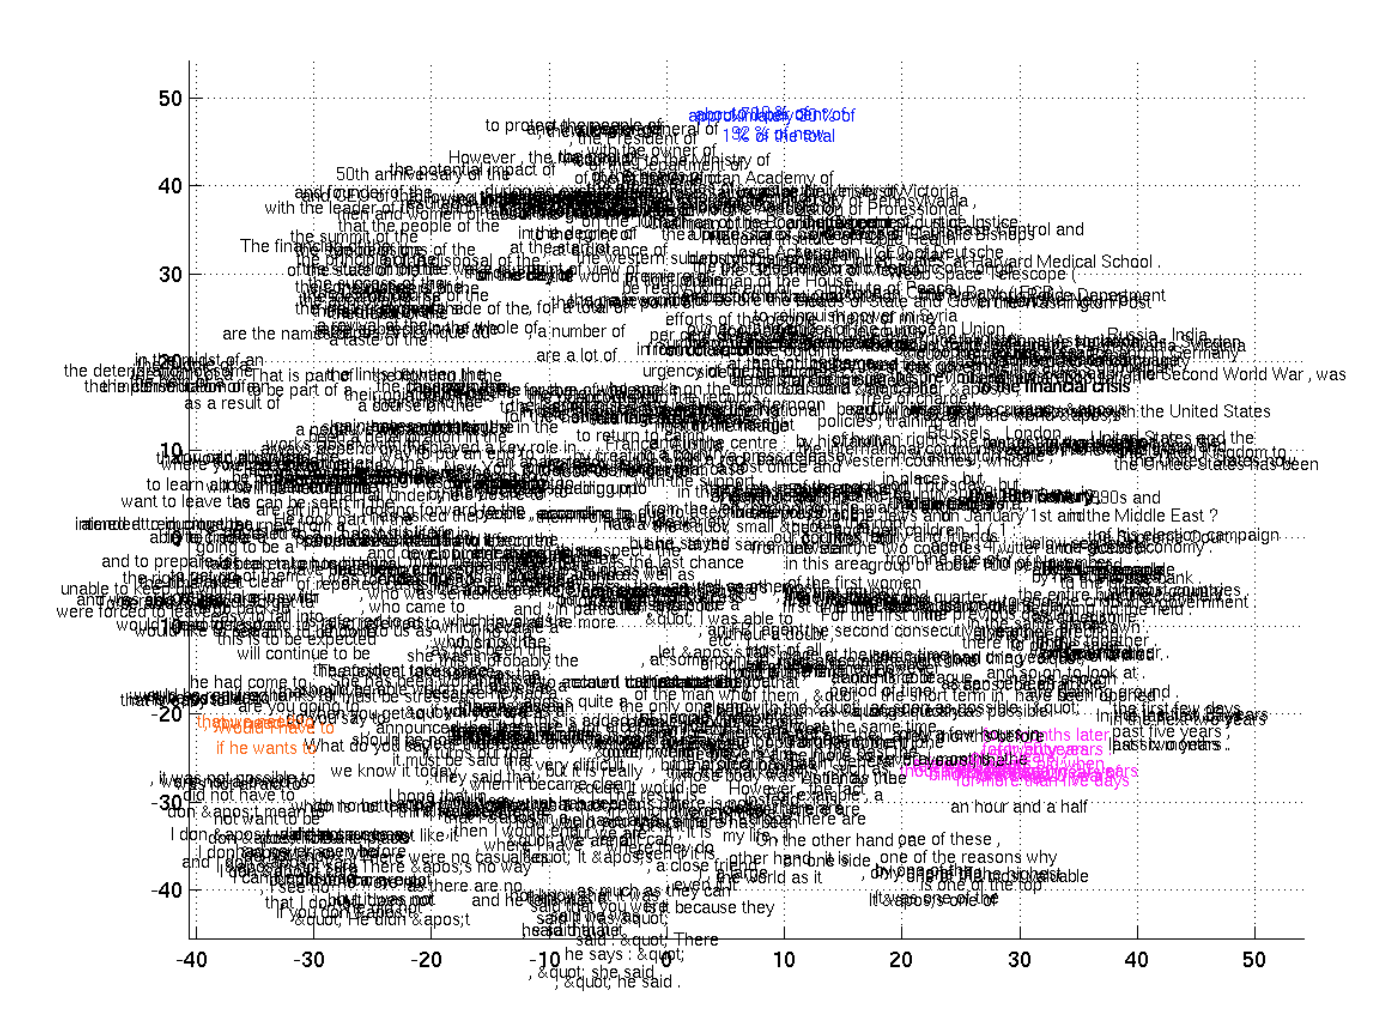
\includegraphics[width=0.3\textwidth]
    				{img/word_embeddings_messy.png} 
    			}}%
    			\caption{Phrase embedded plot}%
    		\label{fig:mnistHintonEmbedded}
	\end{figure}
 		
		Interaction isn't always necessary however, and some attempts have been made to show data in a flat two dimensional representation using dimension reduction, which will be explored in depth a little later. The plot of the MNIST data set, a set of handwritten digits from one to nine, by \cite{Maaten2008} provides a clear non-interactive view of the data where spotting patterns such as the angle deformation of the `1' characters across a class clustering, or spotting simple misclassification becomes easy.
		\par 
		As with exploring two dimensional data its important to remember that there is no one rule that fits all. A less successful example of embedding data within the plot itself is by \cite{Cho2014} who attempt to visualise phrases. Here you can see that the data become messy incredibly quickly, and that perhaps interaction would be a better method of ensuring we retain Olahs principles. 
		\par

		Providing a user with the tools to control the data being visualised is incredibly important in engaging the user in the discovery process. The user must be able to change important network parameters, and immediately see the effects of such a change. They must also be able to compare and contrast different portions of the data through selection, and control the rate at which this change in information is depicted so as to allow them to discover patterns for themselves. 
		\par 		
		 		
	\begin{figure}[H]
    			\centering	
			{{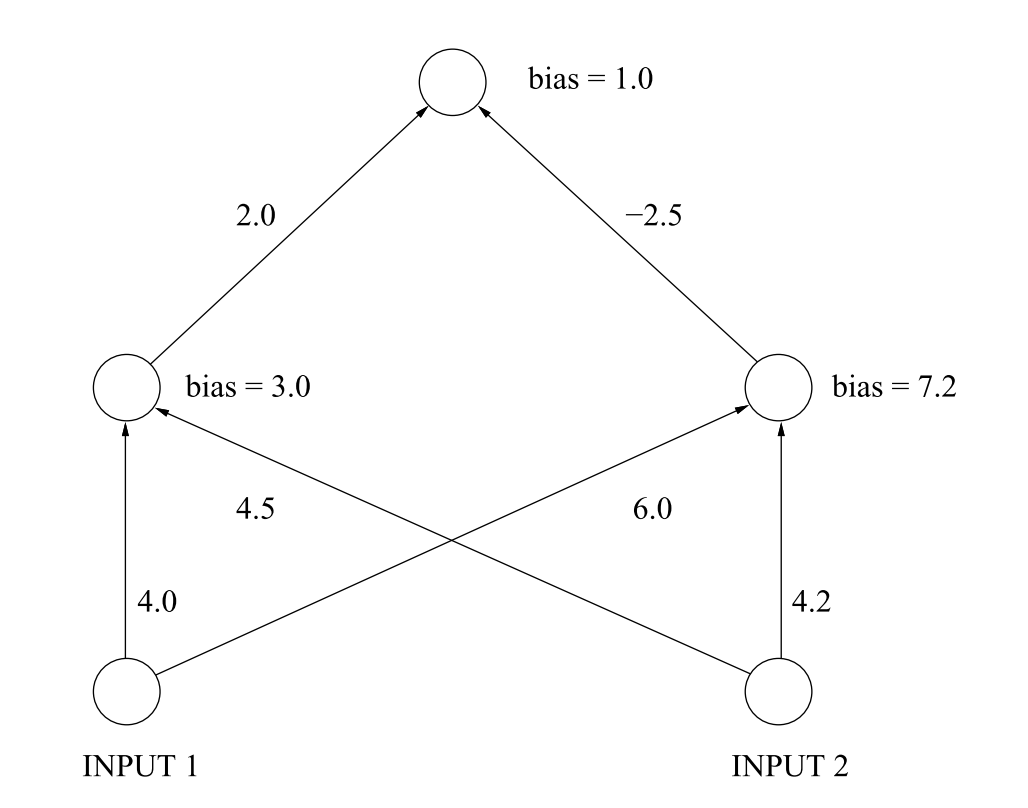
\includegraphics[width=0.3\textwidth]
    				{img/craven_simple_net.png} 
    			}}%
    			\caption{Simple Neural Network}%
    		\label{fig:simple}
	\end{figure} 		
 		
A compelling argument is made by  for interaction when exploring scientific data visually. He shows that there is often a situation where the data is so dense, where there is simply too much to explore in an effective way, that interaction in the only solution; instead hovering over the points and being provided with a tool-tip that demonstrates the points value. Interactive filtering can help, allowing the user to choose some number of easy to visualise classes. 

	\subsection{ANN Visualisation: Early Years}
 		
	 Visualisation has been around helping researchers in neural networks for a long time, and techniques such as the \textit{Hinton diagram} were first demonstrated as early as 1986. This section provides a brief overview of similar techniques from around the nineties, where a number of the techniques are going to be visualisations of fig. \ref{simple}.
		
		\subsubsection{Hinton Diagram}
		 		
 	\begin{figure}[H]
    			\centering	
			{{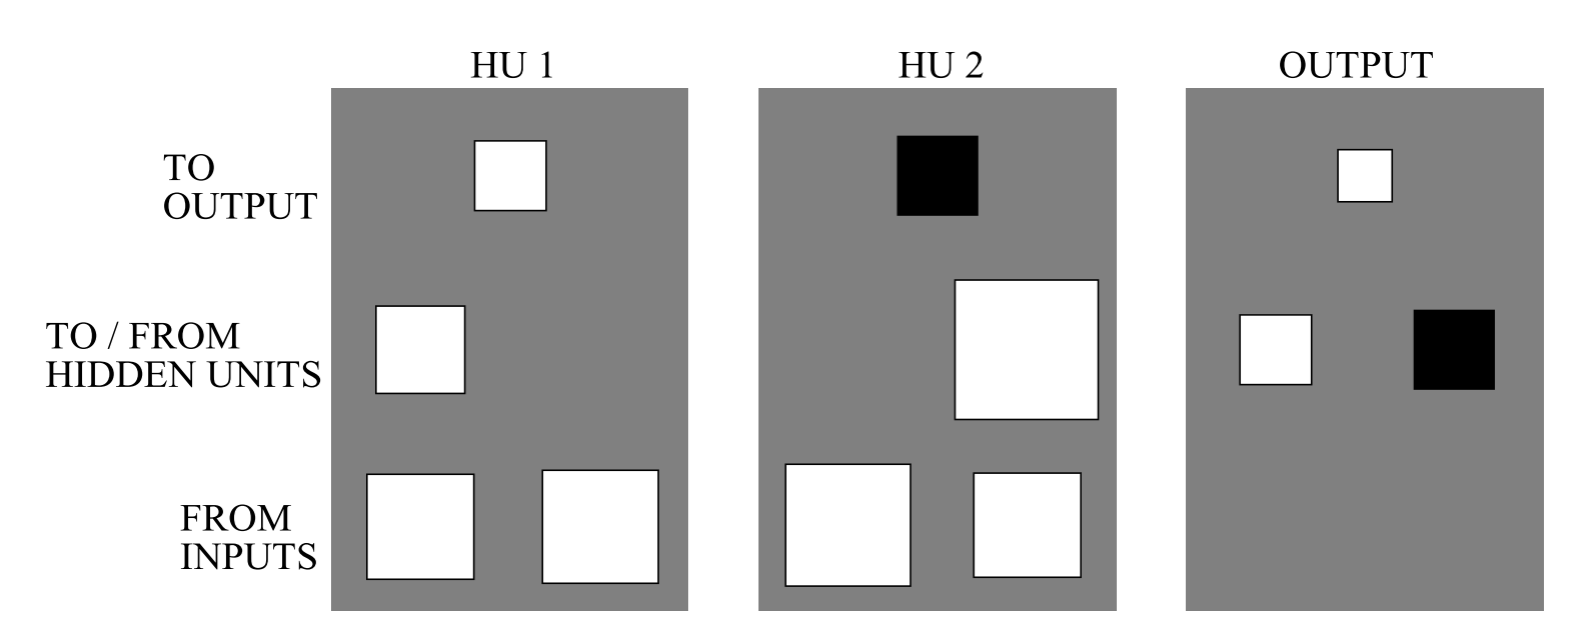
\includegraphics[width=0.3\textwidth]
    				{img/craven_hinton.png} 
    			}}%
    			\caption{Hinton Diagram}%
    		\label{fig:simple}
	\end{figure} 
 		
		One of the first practical visualisations of ANNs was the \textit{Hinton Diagram} \cite{Hinton1986}. It visualises the weights and biases related to a node within a network. Weights are represented as boxes, where its area represents the weights magnitude, and it's shade represents the sign on the weight - white is positive, black is negative. Biases are illustrated as weights from a node back to itself. There is a vague representation of the architecture as output nodes appear at the top of a diagram, hidden nodes are in the middle, and input nodes are at the bottom. However these diagrams are rather unclear, and lack of topological information is a problem. The advantage is they make it easy to see the signs and magnitudes of the weights that contribute to a neurons activation.
		\par 
		
		\subsubsection{Bond Diagram} 
 		
 	\begin{figure}[H]
    			\centering	
			{{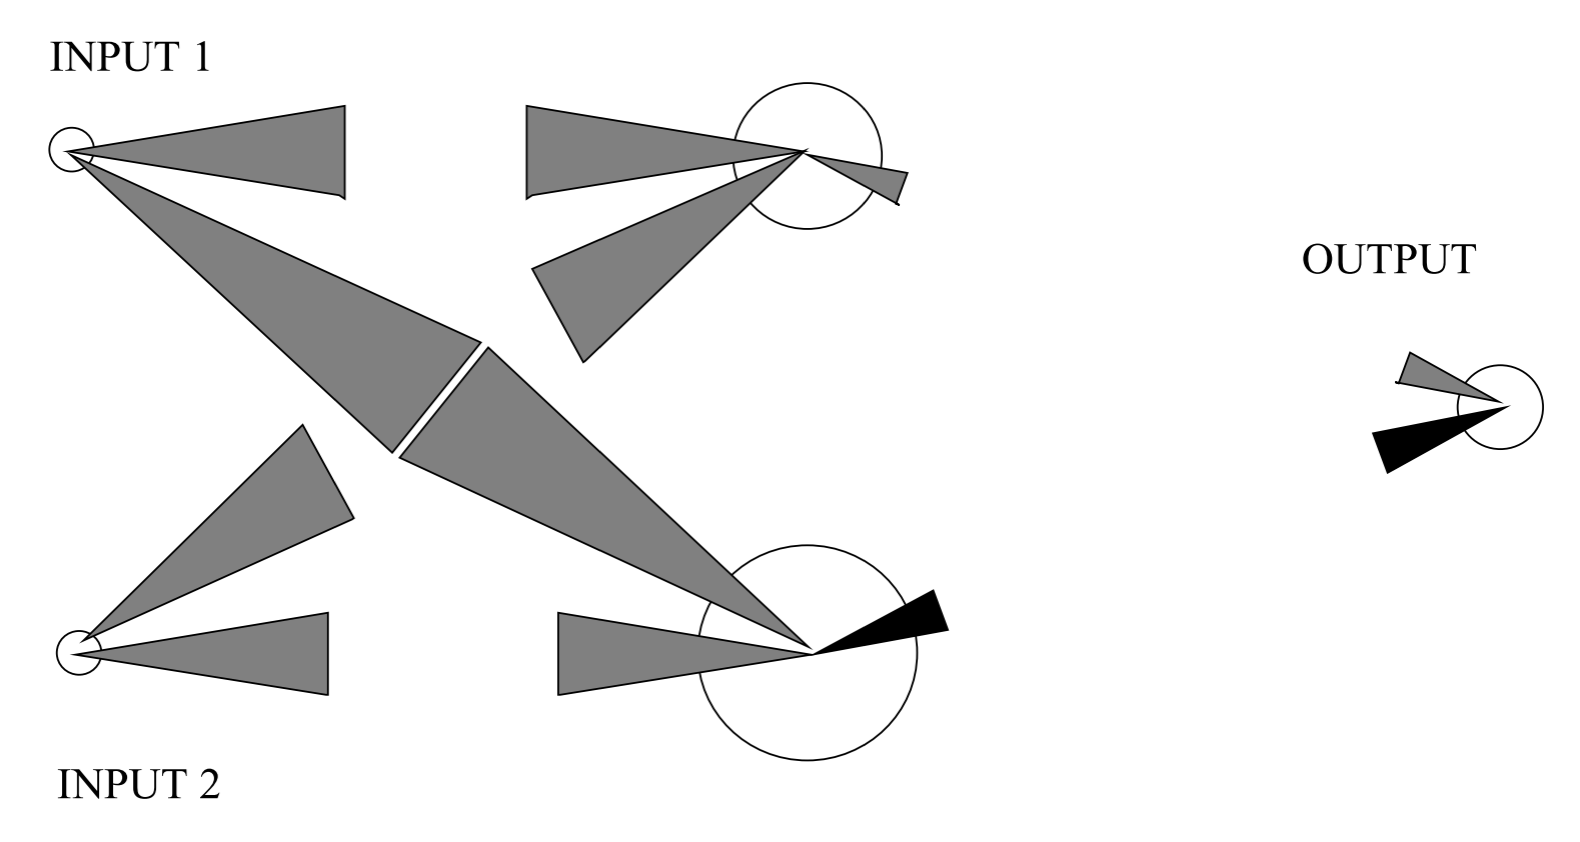
\includegraphics[width=0.3\textwidth]
    				{img/craven_bond.png} 
    			}}%
    			\caption{Bond Diagram}%
    		\label{fig:bond}
	\end{figure} 
 		
		Similar to the \textit{Hinton Diagrams}, the Bond diagram \cite{Wejchert1990} graphically depicts the values of the networks weights and biases. The bond diagram however attempts to make the architecture of the network more clear; a neuron is depicted as a circle, where the diameter of the circle indicates the magnitude of the bias, and triangles connecting the circles represent the weights. The magnitude is indicated by the height of the triangle, and colour depicts the sign. 
		\par 
		While it is perhaps easier to decipher the network structure from the Bond diagram, it is harder to gauge the relative importance of the weights and biases which have been depicted with different shapes. It makes the following question very difficult to answer: ``which input units need to be active in order for the net input to exceed the threshold (bias) of the hidden units?" \cite{Craven1992}, a useful question that Hinton diagrams are far better at answering.
		\par 
		
		\subsubsection{Hyperplane Diagrams}
 		
 	\begin{figure}[H]
    			\centering	
			{{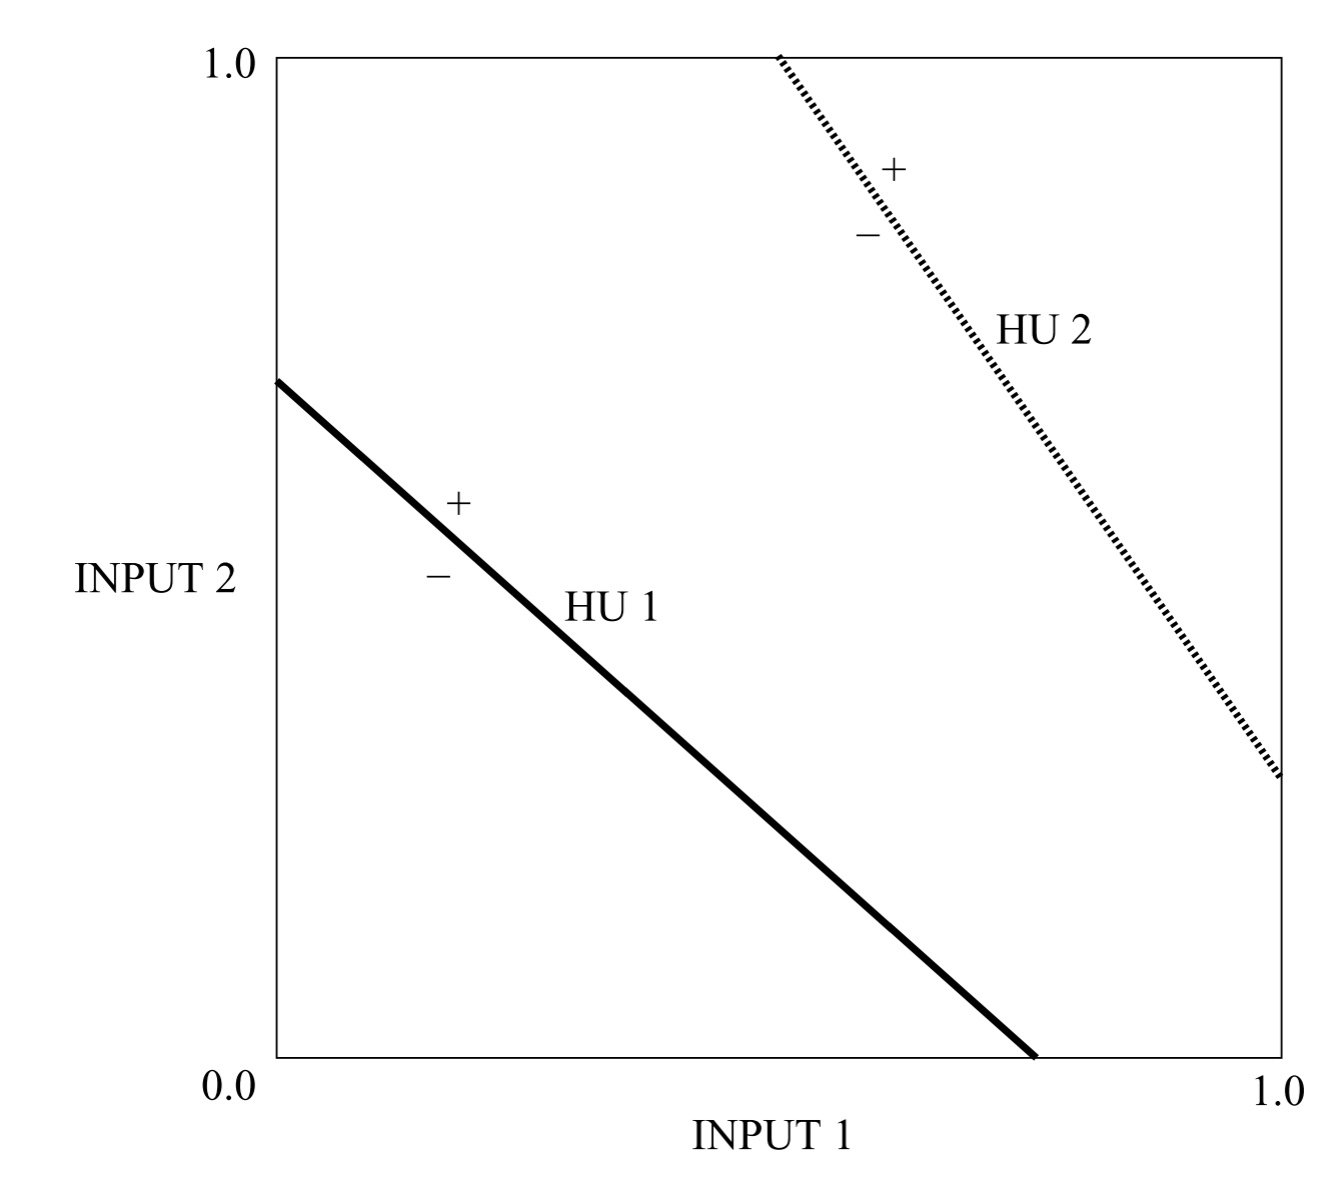
\includegraphics[width=0.3\textwidth]
    				{img/craven_hyperplane.png} 
    			}}%
    			\caption{Hyperplane Diagram}%
    		\label{fig:bond}
	\end{figure} 
 		
		A hyperplane depicts the `threshold' of a decision surface. As this hyperplane moves throughout the training process, visualising the hyperplane as it moves can be a useful method to get an understanding of what a neuron is learning \cite{Munro1992}. Neurons that appear in the same layer can have their hyperplanes shown in the same diagram due to a sharing of input space, making comparison easy.
		\par 
		One issue with this hyperplane representation is that while accurately representing a threshold function acting on a two-dimensional input space, the diagrams fall down when compared with most contemporary ANNs that require multiple dimensions (>3) to be shown and more commonly use continuous transfer functions such as  the sigmoid - which requires a gradual, rather than a sudden, division of the input space. That said, it can be assumed that the hyperplane is a close approximation of the gradual boundary and so can still provide useful observations.
		\par 
		
		\subsubsection{Response-function plots}
		
 	\begin{figure}[H]
    			\centering	
			{{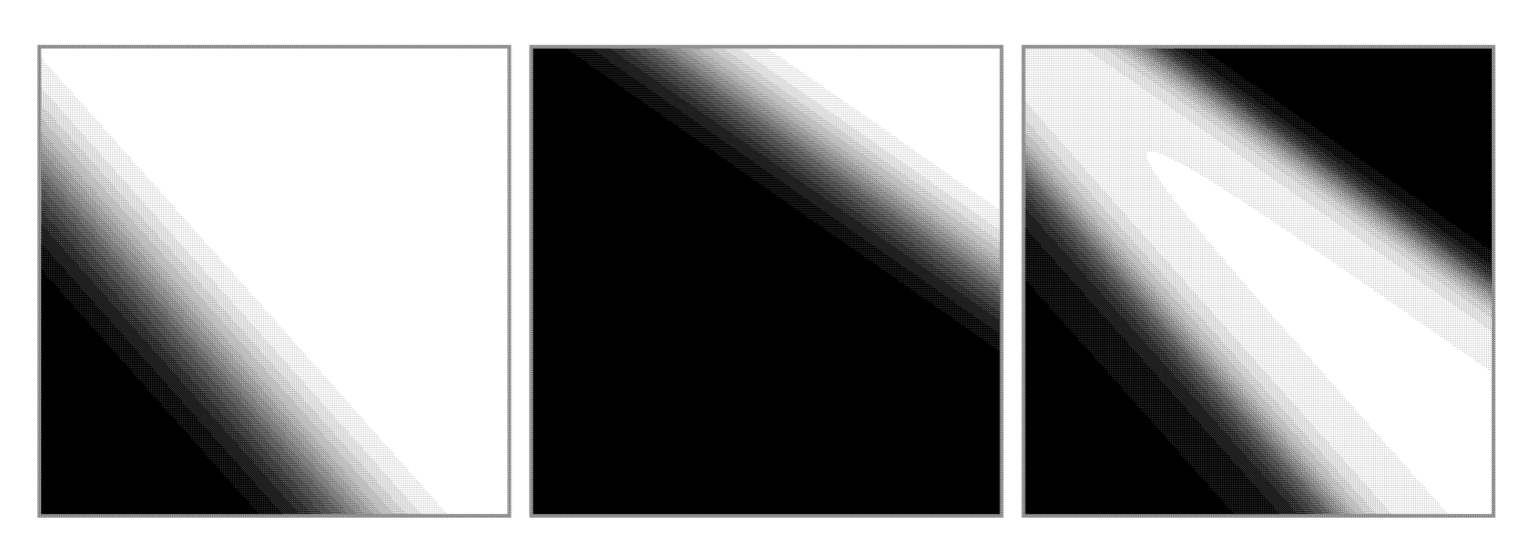
\includegraphics[width=0.3\textwidth]
    				{img/craven_gradient.png} 
    			}}%
    			\caption{Response Function Plot}%
    		\label{fig:bond}
	\end{figure} 
 		
		Response-function plots are very similar to hyperplane diagrams - they also display the decision surface. They differ in their solving of the issue of the gradual boundary. Instead of displaying the space using a hyperplane, the space is displayed as a gradient of values to indicate the resulting activations.
		\par 
		Interestingly, both the Response-Function Plots and the hyperplane diagrams show the space between two successive layers of neurons. This provides only a fraction of information about the network, and problematically may lead to false assumptions about it. One way to address this is to describe the decision surface not just on the layer below, but across all previous layers of the input space.
		\par 
		
		\subsubsection{Trajectory Diagrams}
 		
 	\begin{figure}[H]
    			\centering	
			{{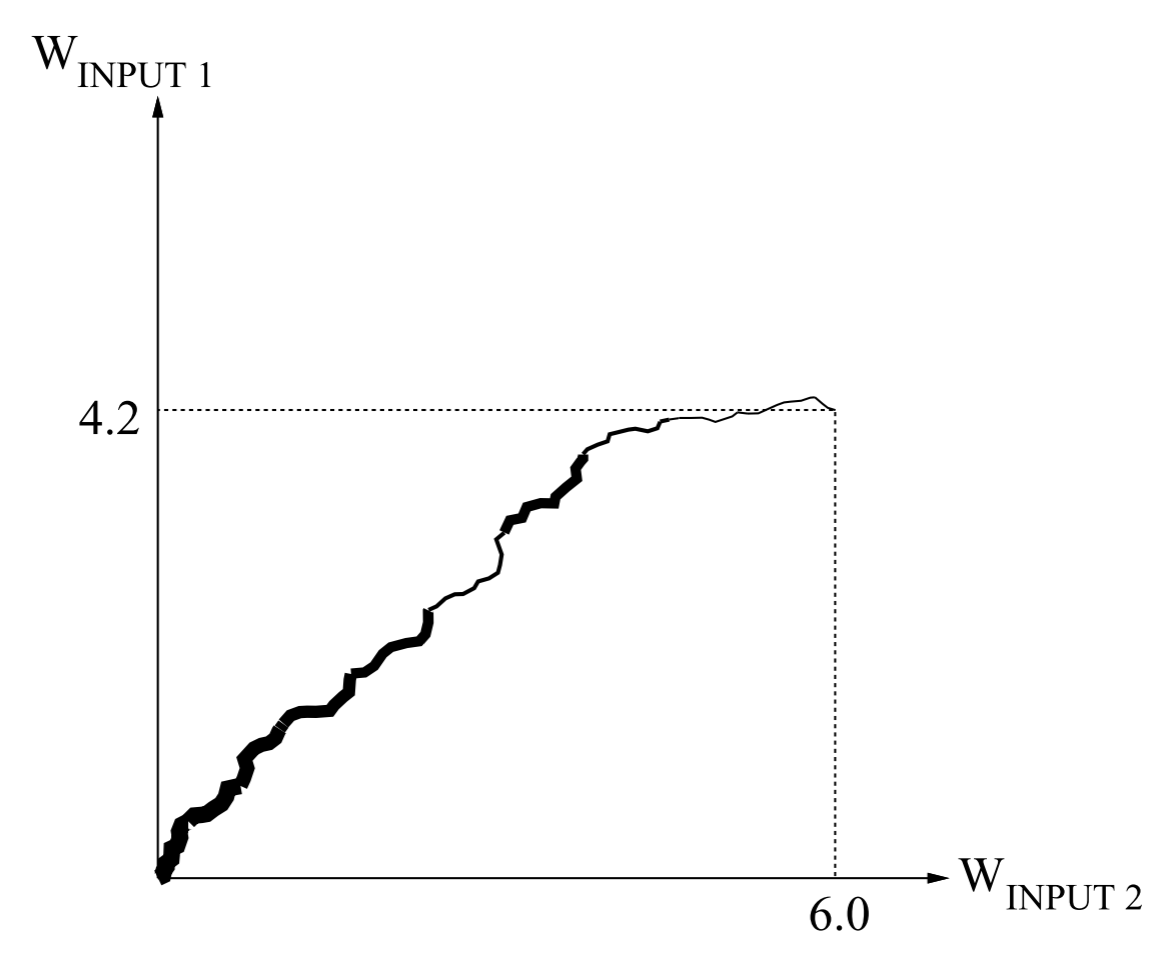
\includegraphics[width=0.3\textwidth]
    				{img/craven_trajectory.png} 
    			}}%
    			\caption{Trajectory Diagram}%
    		\label{fig:bond}
	\end{figure} 
 		
		Trajectory Diagrams \cite{Wejchert1990} depict the change in weight space and in error over a neuron during training. These diagrams use the incoming weights of a neuron to create the axes of a plot. During training as the weights change they are visualised as a trajectory in the weight space. The error at a given time is indicated by the thickness of the trajectory line.
		\par 	
		Again, along with many of these other early visualisation methods, the weakness of the trajectory diagram is its inability to display weight spaces of more than three dimensions. There have been efforts to combine dimensionality visualisation with trajectory diagrams - such as using radially projected axes, however this is fairly unsuccessful \cite{Craven1992}. 
		\par 
		
		\subsubsection{Lascaux}
 		
	\begin{figure}[H]
    			\centering	
			{{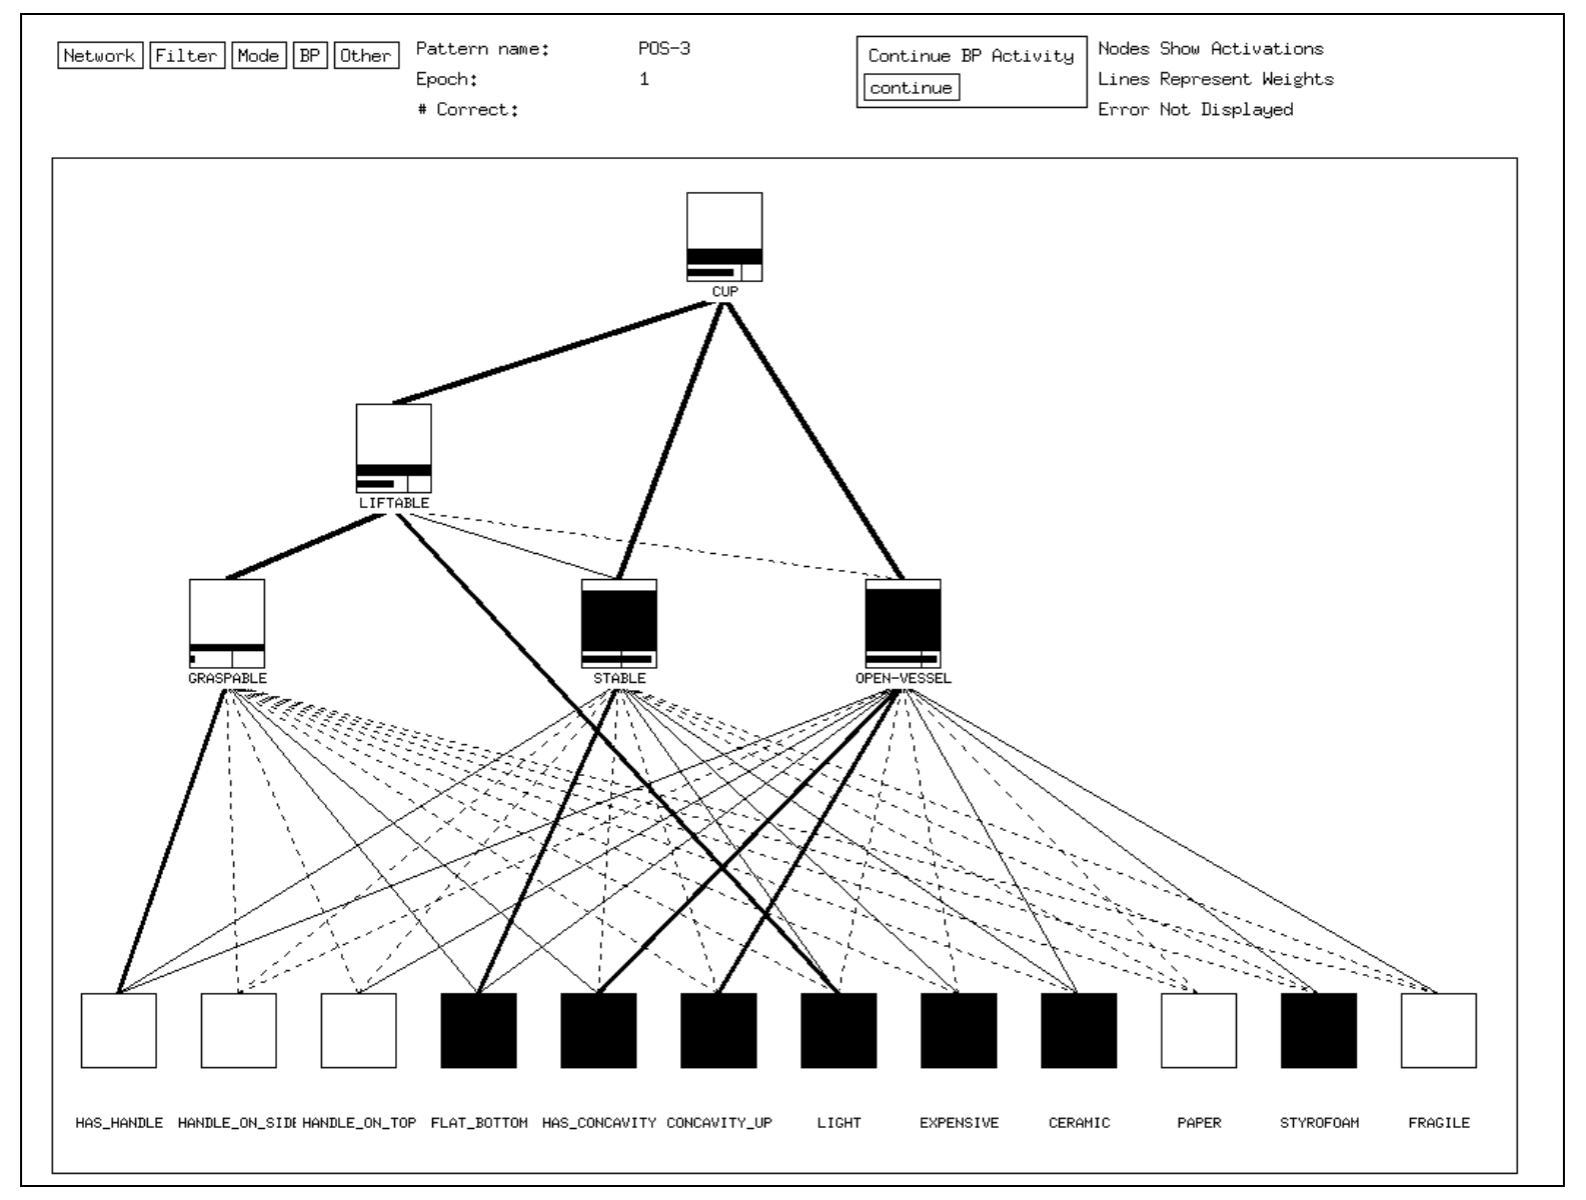
\includegraphics[width=0.3\textwidth]
    				{img/craven_weights.png} 
    			}}%
    			\caption{Lascaux Clip}%
    		\label{fig:lascaux}
	\end{figure}  		
 		
		Lascaux is a visualisation tool proposed by \cite{Craven1992} that aimed to clearly display the topology of a network. Here, each neuron is represented as a box and network weights are represented by interconnecting lines. A weights magnitude is visualised by the thickness of a line, and the positive or negative signs are visualised as solid and dashed lines respectively.
		\par 
		The tool depicts a range of information it one place. Activation of each neuron is show as a vertical bar within the neuron `box'; a horizontal bar shows the net input relative to a threshold - shown as a line intersecting the bar; error is another vertical bar within the neuron box; a separate diagram shows the error propagating as connections between these boxes - where thickness describes magnitude.
		\par 
		The issue with \textit{Lascaux} is that too much information is being displayed in a small space ineffectively. The approach uses standard two dimensional visualisation techniques, and simply squashes them into a neural network architecture. This makes the topology easier to understand, but at the sacrifice of more important elements.

	\subsection{ANN Visualisation: Parameters}
	As visualisation within the neural network community became more popular, a number of other visualisations were developed.
		\subsubsection{Weights and Connection}
		When representing weights, it is important to consider the analytical impact of a visual decision. \cite{Streeter2001} visualises the topology of the network but doesn't clearly show the weights themselves. This can lead to confusion when assessing the importance of a neuron. Consider for example a neuron that has appears to have a high value in one layer, however is subsequently cancelled out by low weights deeper within the network.
	\par 
	One problem here is that since the absolute values of the weights are used, the result does not provide the direction of the relationship. 
	\par 
		
	\begin{figure}[H]
		\centering 
    		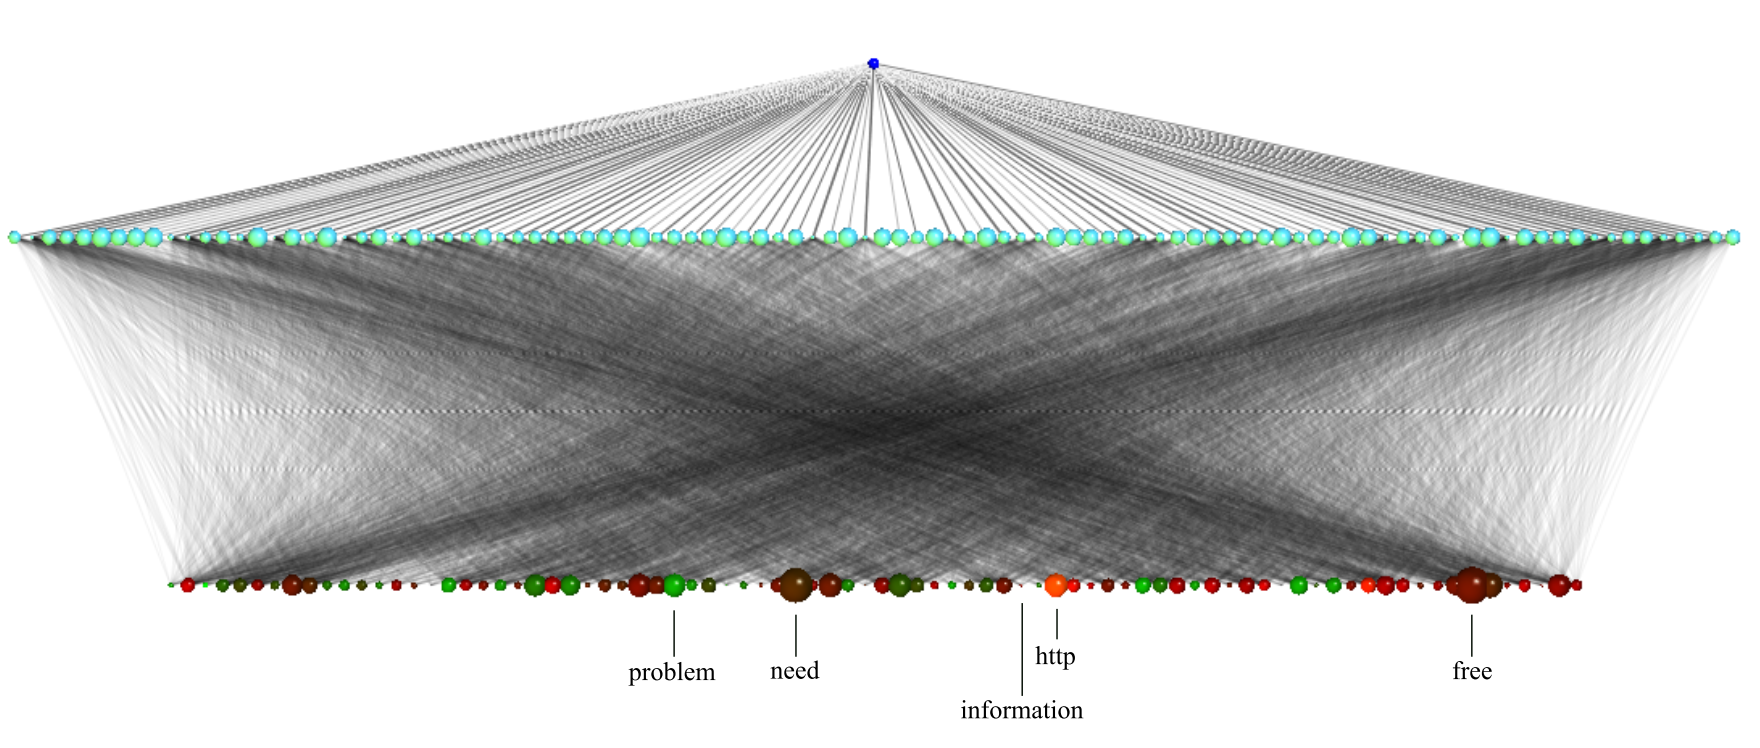
\includegraphics[width=0.7\textwidth]{img/tzeng_large_map.png} 
    		\caption{Tzeng Map}%
 	\end{figure}
 	
	\cite{Tzeng2005} based on the work of 	\cite{Garson1991} and \cite{Goh1995} sought to solve this problem in a different way; by visualising the weights with line-thickness between nodes, thus making it easy to identify when a node is insignificant regardless of the magnitude of weights applied to it.
	\par 
	In addition 	\cite{Tzeng2005} propagate all of the layers influence through the network by multiplying each weight between the previous layers with those of the successive layers which connect to the same node. Here, they represent the contribution of a specific hidden node by adjusting the diameter of the circle visualising the neuron in their visualisation. The contribution of the input unit $ i $ to the output unit $ o $ through a hidden unit $ j $ is computed by multiplying the input-hidden weight strength and the hidden-output weight strength:
$ r_{ijo} = w_{ij} \times w_{jo} $, and the relative contribution from each input node $ k $ to a hidden node $ j $ can be represented as:
		$$
		r_{ijo} = 
		\text{ $ \frac{|C_{ijo}|}{\sum\limits_{k=1}^m |C_{kjo}| } $ }
		$$ 
	where the total contribution from an input node $ i $ is: 
		$$
		S_{i} = 
		\text{ $ \sum\limits_{j=1}^n r_{ijo} $ }
		$$ 
	and the relative importance of an input node is therefore:
		$$
		RI_{i} = 
		\text{ $ \frac{S_{i}}{\sum\limits_{k=1}^m S_{k} } $ }
		$$ 
	 \par 
 		
	 This combination of statistical analysis and weight representation allows for a visualisation that demonstrates not only the raw data, but an abstraction that is more useful to the researcher given the relative importance of the nodes, and significance of the data - while still providing an architectural understanding of the network. This combination of mathematics and visualisation is one that continues across a number of other visualisation techniques for neural networks.
	 
	\subsubsection{Features}
		Visualising the features of a CNN to gain an intuitive understanding about its internal behaviour is becoming commonplace, it is mostly limited to the simple visualisation of the 1st layer where projections to the pixel space are relatively easy to achieve. However there are exceptions, and a small number of researchers have developed methods for visualising deeper hidden layers.
		\par 
		\textbf{\cite{Erhan2009}} sought to find the optimal stimulation of a unit activations through gradient descent in the image space. This has been criticised as difficult to obtain due to the need for careful initialization, and the lack of information conveyed about a units invariance. 
		\par 
		\textbf{\cite{Le2010}} show how the Hessian of a given node may be computed numerically around an optimal response - thus fixing the formers shortcomings by providing a view of invariances. The issue with this approach is with the higher layers where invariances become increasingly complex and are thus poorly encoded in their quadratic approximations. 
		\par 
		\textbf{\cite{Vondrick2013a}} use feature inversion algorithms, where an image is featurized and then recovered to a transformed but decipherable format - again to give intuitive access to abstract feature representations formed by the network. Using this technique they discovered single deep neurons that were trained to respond to faces and bodies, both human and animal. 
		\par
		
		\begin{figure}[H]
			\centering	
    			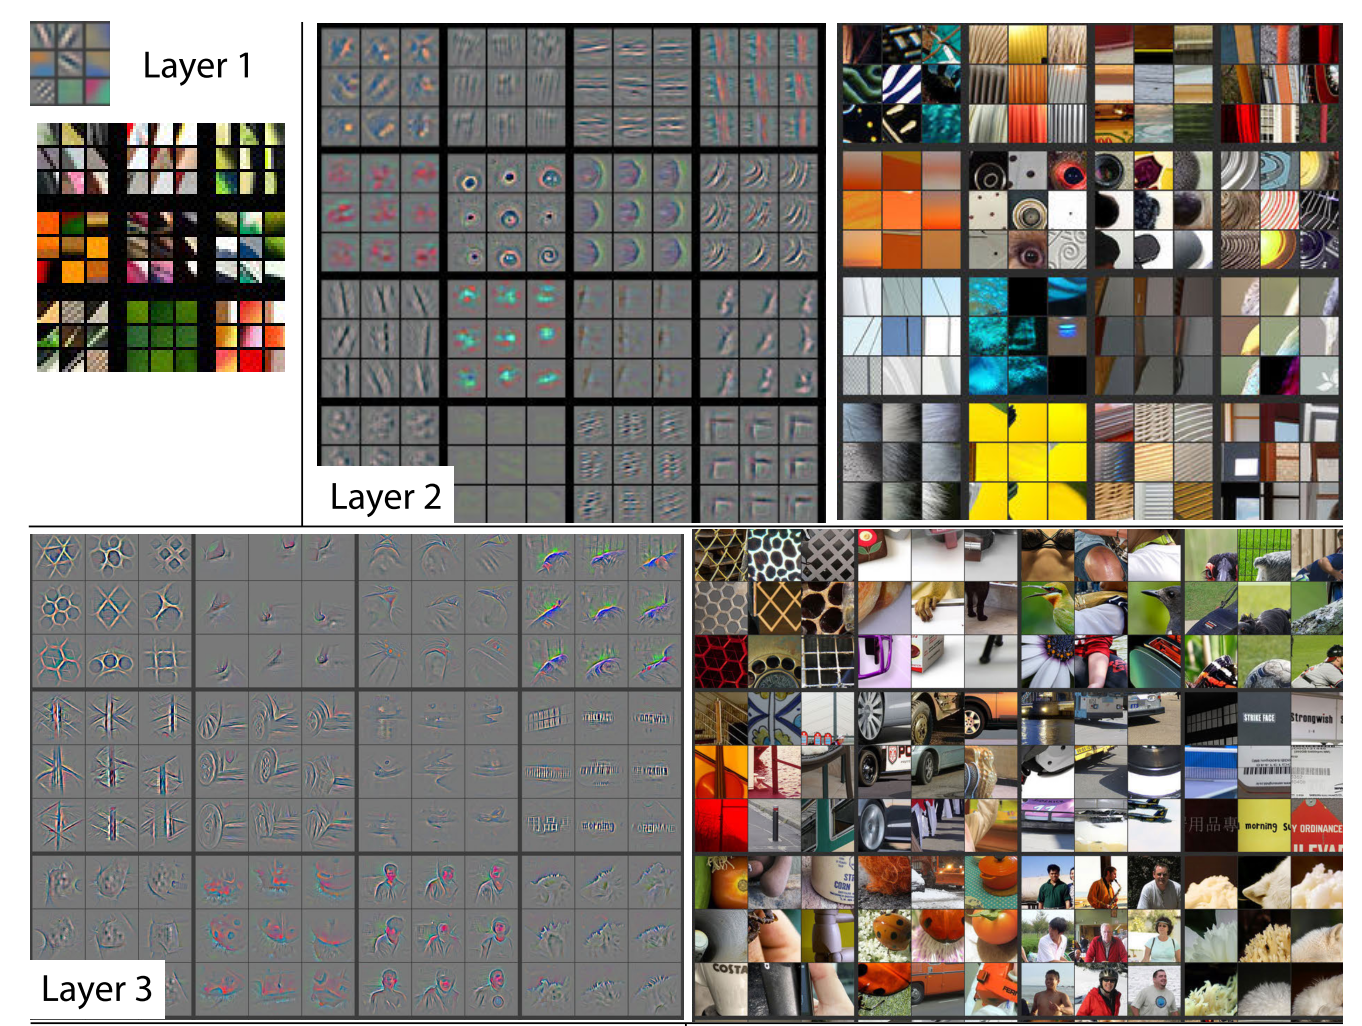
\includegraphics[width=0.5\textwidth]{img/zeiler_deconv.png} 
    			\caption{Zeiler Deconv}%
 		\end{figure}
 		
		\textbf{\cite{Zeiler2013}} provide a technique called \textit{Deconvolution} \cite{Zeiler2011} which effectively reverses a convolutional network. Deconvolution is a type of feature inversion that renders re-weighted versions of inputs, highlighting areas, patterns and textures of an image deemed most important by a particular part of the network. It essentially approximates a reconstruction of the input of each layer from its output.
		\par
		\textbf{\cite{Donahue2013}} show visualisations identifying patches in a dataset that cause strong activations at higher layers in a network. However these have been criticized as only producing a cropped version of the input images, so are limited learning tools. 
		\par 
		\textbf{\cite{Simonyan2013}} describe a technique for visualising class models learnt by CNNs. Given a CNN and a class of interest, the visualisation method numerically generates an image that is representative of the class in terms of the CNN class scoring model.
		\par 
		Clearly with such a lot of attention placed on visualising featurizations, it's a significant opportunity to learn about the networks. It's important to realise however that one of the above is not necessarily better than the others: each show a different element of the featurization, and as experts still know relatively little about the behaviour of ANNs it's important to not discard any of these visual aids rashly.
		
		\subsubsection{Classification Uncertainty}
		 		
 	\begin{figure}[H]
    			\centering	
			{{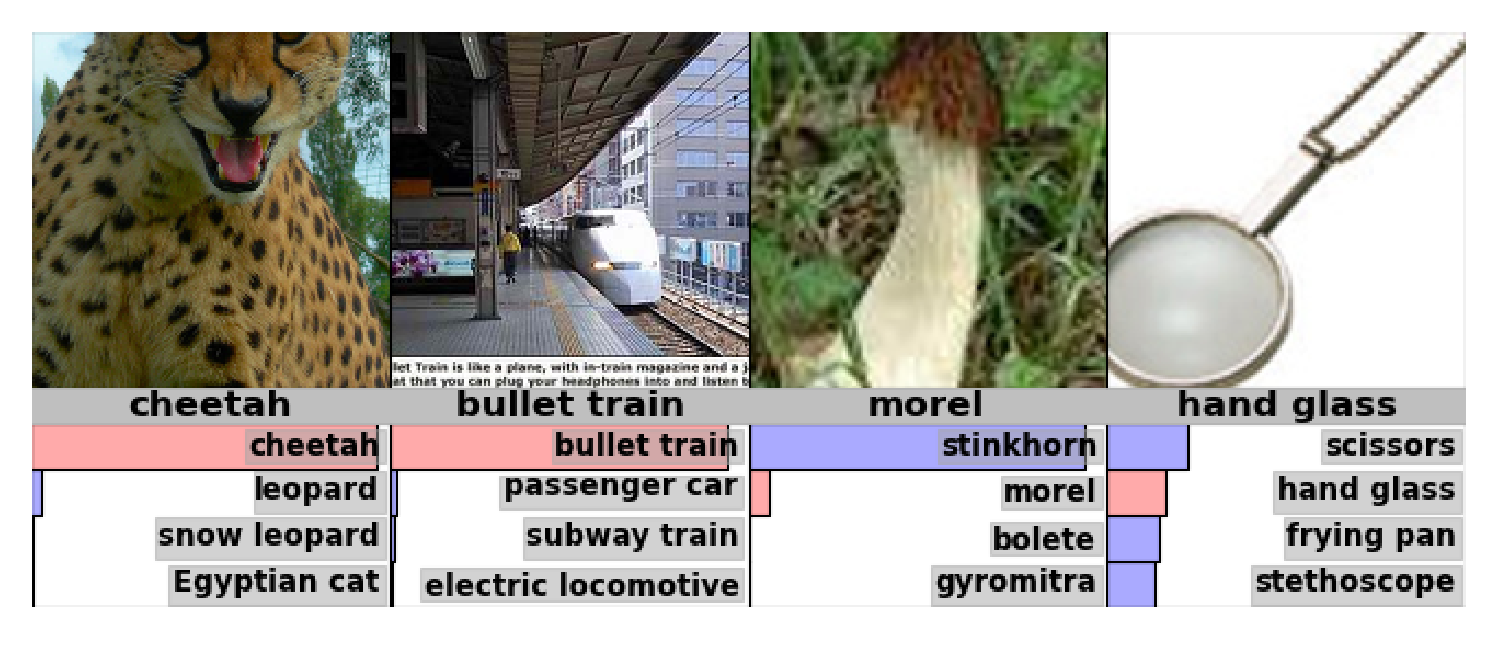
\includegraphics[width=0.3\textwidth]
    				{img/hinton_probability.png} 
    			}}%
    			\caption{Class probability distribution}%
    		\label{fig:lascaux}
	\end{figure}
 		
 		During classification, a neural network outputs a value representation of the uncertainty of its decision, this is usually represented as a probability distribution over the outputs. 

	 	\par 
		 High and low values indicate clear classification, and central values indicate high uncertainty and that the data is difficult for the neural network to classify. \cite{Tzeng2005} uses a parallel coordinate system to show this uncertainty, and uses colour to highlight data that is difficult for the system to classify.
		\par 
		\cite{Talbot2009} shows this uncertainty, in a confusion matrix to visually represent a classifier as a graphical heat-map. They also implement an interaction system that allows users to partition the class space into multiple subsets, allowing experts to get both global and local level views of the data.
 		 
 		 \begin{figure}[H]
    			\centering	
    			\subfloat[Covariance Matrix]											{{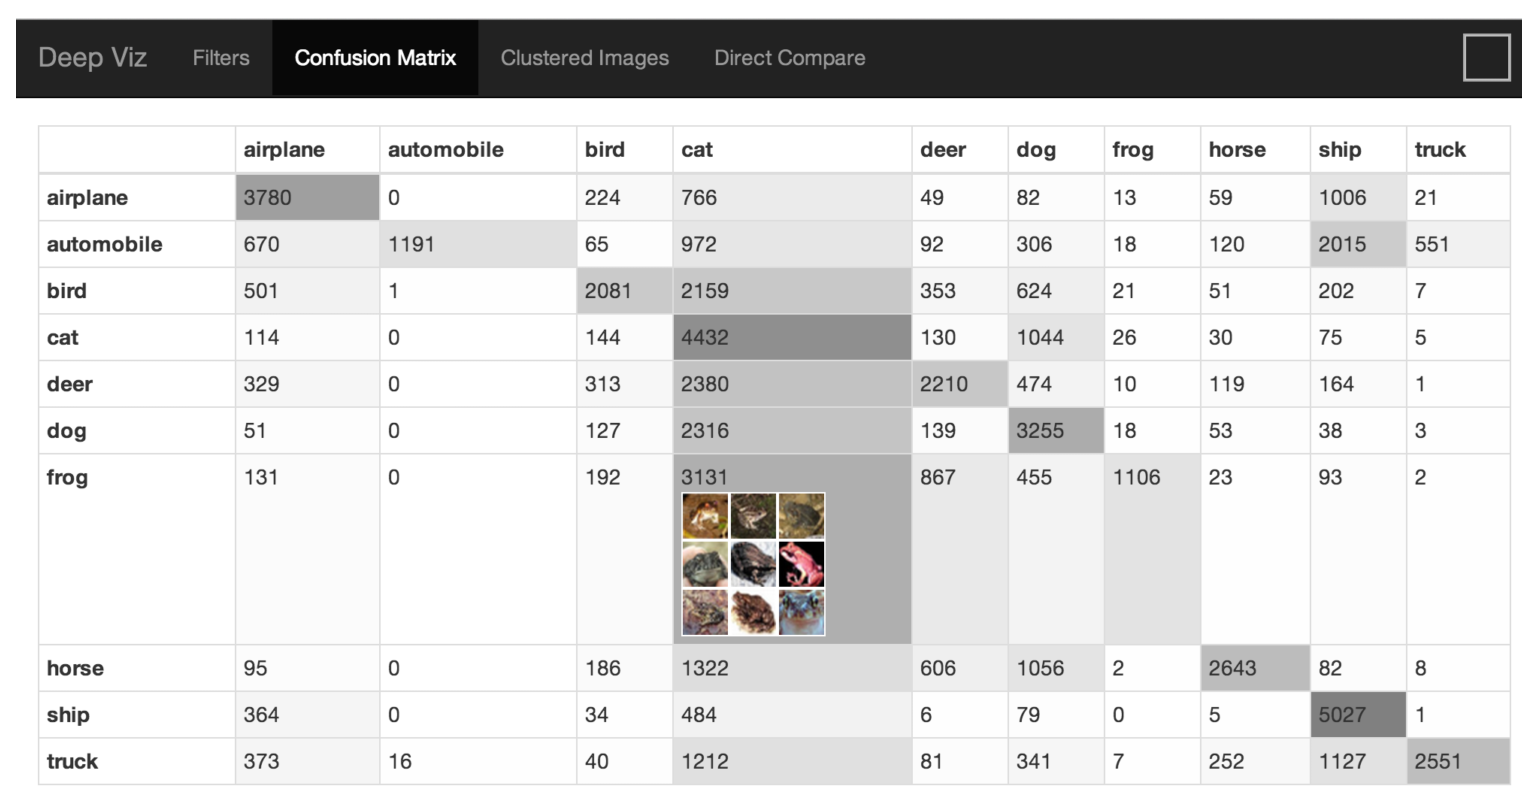
\includegraphics[width=0.3\textwidth]
    				{img/deepviz_covariance.png} 
    			}}%
    			\qquad
    			\subfloat[Parallel coordinate system]
    			{{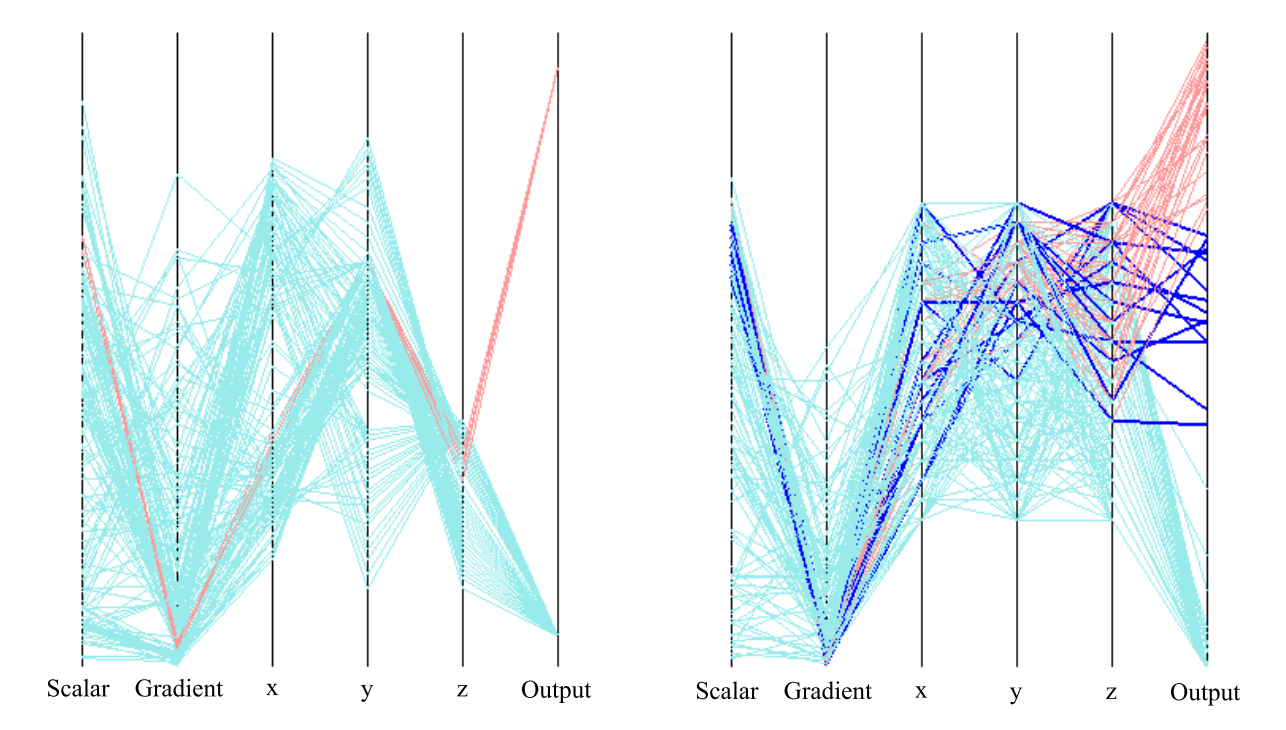
\includegraphics[width=0.3\textwidth]
    				{img/tzeng_parallel.png} 
    			}}%
    			\caption{ }%
    			\label{fig:studentprofile}
		\end{figure}
		
		
		\par 
		A confusion matrix represents classification results by plotting the columns as an instance's predicted class and the rows an instance's true class. They reveal trends and patterns in classification results and thus the behaviour of the classifier itself. Usefully, a confusion matrix is entirely model agnostic and can therefore allow direct comparison between different instances of trained models.
		
	\subsection{ANN Visualisation: Multiple Dimensions}
	Human brains are incredibly good at understanding two and three dimensions, with a bit of effort its possible to reason in four. An inherent difficulty with understanding ANNs is that we cannot truly hope to understand multi-dimensional problems.
	\subsubsection{Visualising High-Dimensional Data}
	Visualising high-dimensional data is a very important problem in several different domains that each deal with data of widely varying dimensionality. It is therefore a very well explored problem and a number of techniques for visualising high-dimensional data exist, a summary of which was composed by \cite{Cristina2003}.
	\par 
	This covers techniques by a number of different authors;	
		\par
		
 	\begin{figure}[H]
    			\centering	
			{{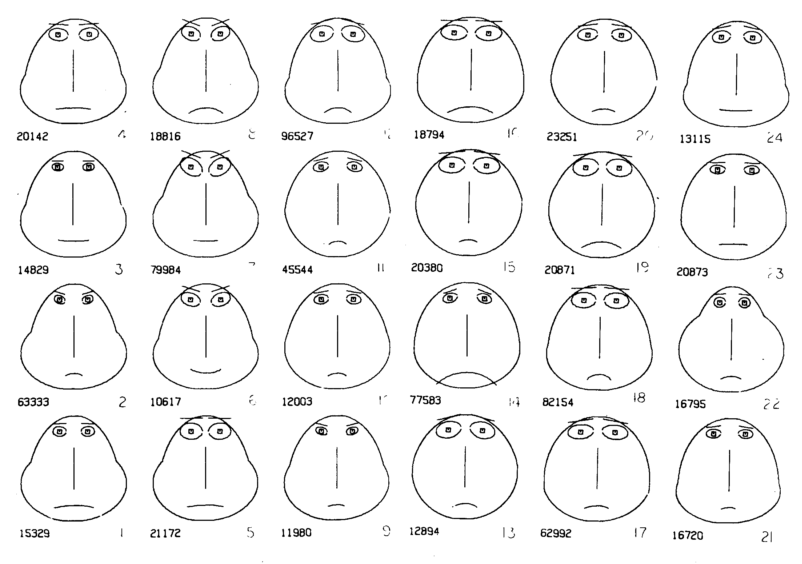
\includegraphics[width=0.3\textwidth]
    				{img/chernoff_faces} 
    			}}%
    			\caption{Chernoff Faces}%
    		\label{fig:lascaux}
	\end{figure}
 		
		 \textit{Chernoff Faces} are iconographic visualisations of faces by \cite{Chernoff1973}; each point in k-dimensional space, $ k < 18 $, is represented by a cartoon of a face whose features, such as length of nose and curvature of mouth, correspond to points in the data. Thus every multivariate observation is visualized as a computer-drawn face. This presentation makes it easy for the human mind to grasp many of the essential regularities and irregularities present in the data. This is a rather outdated approach.
		 \par
 		
 	\begin{figure}[H]
    			\centering	
			{{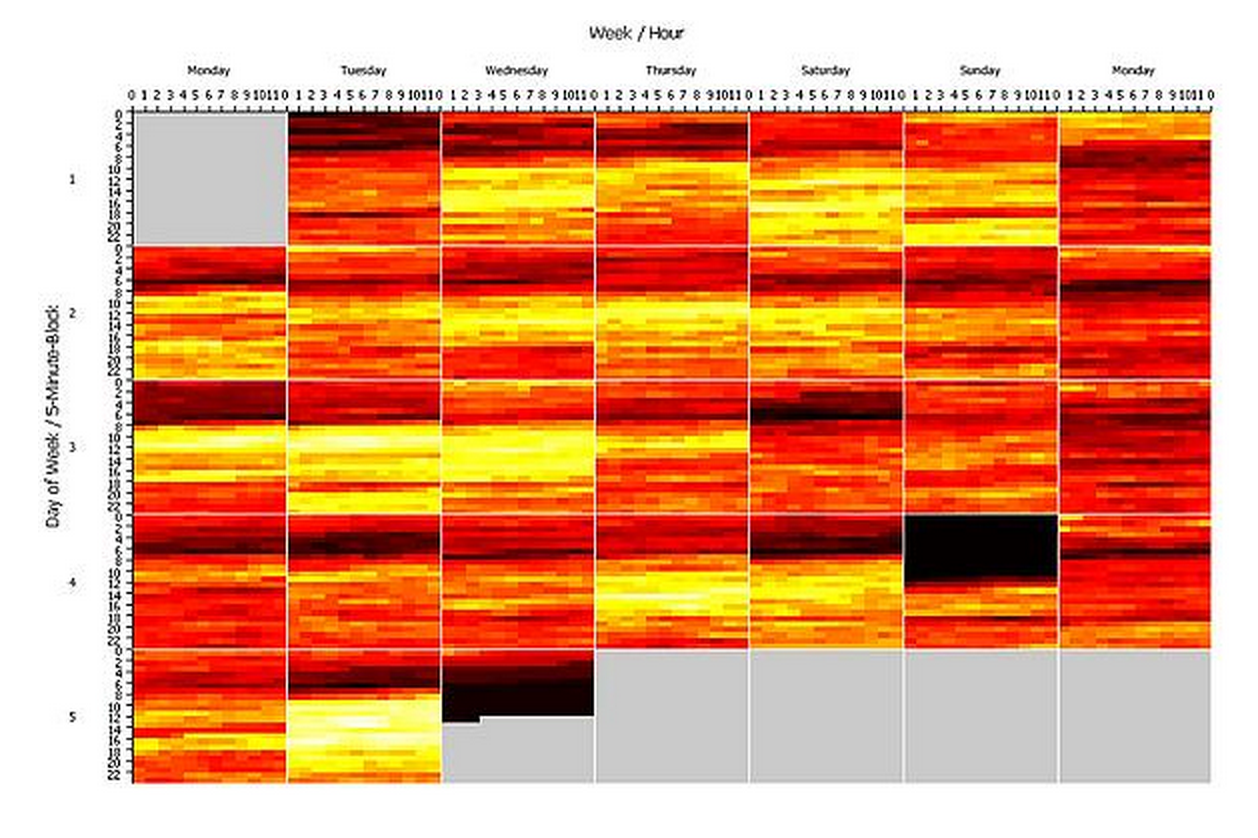
\includegraphics[width=0.3\textwidth]
    				{img/kiem_pixel_two} 
    			}}%
    			\caption{Pixel Based Techniques}%
    		\label{fig:lascaux}
	\end{figure}	
 		
		\textit{Pixel Based}; represent as many data objects as possible on the screen at the same time by mapping each data value to a pixel of the screen and rearranging those pixels to suit the source \cite{Keim2000}. One example is to use a gradient of colour to represent the value of a data-point, and multiple dimensions may be show in different as slices.
		\par 
		 		
	\begin{figure}[H]
    			\centering	
			{{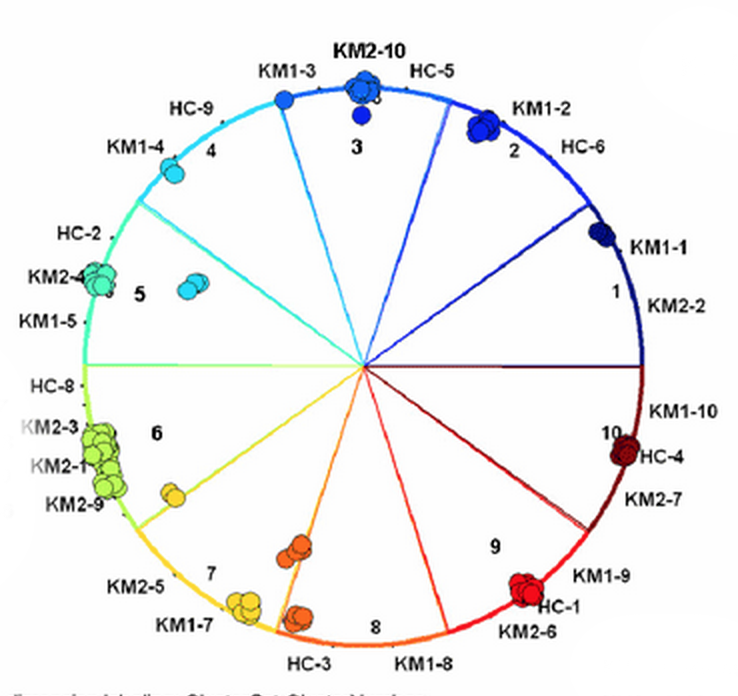
\includegraphics[width=0.3\textwidth]
    				{img/battista_vertices} 
    			}}%
    			\caption{RadViz}%
    		\label{fig:lascaux}
	\end{figure}	 		
 		
 		
		\textit{Radial Coordinate Visualisation} was designed by\cite{Hoffman1999}; for an n-dimensional visualization, n lines emanate radially from the center of a circle and terminate at its perimeter, each line associated with one attribute. The points that sit in amongst the radial portions represent the data described between the dimensions in a similar way to an x-y plot.
		
	\par 
	While these tools do have their uses as visualisation techniques, when it comes to exploring the high-dimensional data of neural networks they have been criticized \cite{Maaten2008} as simply providing the tools to \textit{display} more than two data dimensions, and leave a more difficult task of interpretation to the viewer. With dimensions of real-world data used in DNNs often in the thousands, these techniques may provide limited insight.

		\subsubsection{Dimensionality Reduction}
		Dimension reduction differs from dimensionality visualisation, in that instead of visualising the multiple dimensions of a dataset in a format such as those already described, it actually converts the high-dimensional data set  $ X = \{ x_{1}, x_{2},..., x_{n} \} $ into a low-dimensional data set that can then be displayed easily in a standard recognisable formats such as the scatter plot. Dimensionality reduction aims to preserve as much of the significant structure of the data in higher-dimensions as possible while generating a low-dimensional representation that is easier for the user to interpret. This is fundamentally important for neural nets.
		\par 
		It is possible to draw a notion of how successful this dimensional reduction is by assuming that for any two data points, $ x_{i} $ and $ x_{j} $ there are two notions of distance between them that we can compare. First, is the distance between those points in the representation space, for example the L2 distance $ d(x_{i,j}) = \sqrt{\sum\nolimits_{n} (x_{i,n} - x_{j,n})^2 } $, and the other is the  distance between the points in the visualisation, $ d_{viz}(x_{i,j}) $, such that a cost function of the visualisations success can be defined.
		\par  		
		If the cost $ C $ is high, then the distances are dissimilar to the original space, if low they are similar, and if zero the visualisation is a perfect representation. It's almost impossible however to get a perfect representation in all aspects, so different cost functions provide different compromises, and insights. Once the cost function is decided upon, then there simply exists an optimisation problem that can be tackled though a standard process such as gradient descent to ensure that  points are optimally visualised with respect to the cost function. The cost function for standard Multi-dimensional Scaling \cite{Torgerson1952} is shown below: 
		$$
			C = 
			\sum\limits_{i \neq j}
			[d(x_{i,j}) - d_{viz}(x_{i,j}) ]^2
		$$
		\par 
		Another reduction method is Sammon's mapping \cite{Sammon1969}, which aims tries harder to preserve the distances between nearby points than those further away. If the two points are twice as close in the original space than  two others, it is twice as important to maintain the distance between them. This emphasises the local structure at the compromise of the global structure in the data:
		$$
			C = 
			\sum\limits_{i \neq j}
			\frac{ [d(x_{i,j}) - d_{viz}(x_{i,j}) ]^2 }					{d(x_{i,j})}
		$$
		For some data structures this doesn't work particularly well, so another alternative is to use graph based visualisation. Here its possible to explicitly specify the aim of the dimensionality reduction; preserve local structure. 
		 		
 	\begin{figure}[H]
    			\centering	
			{{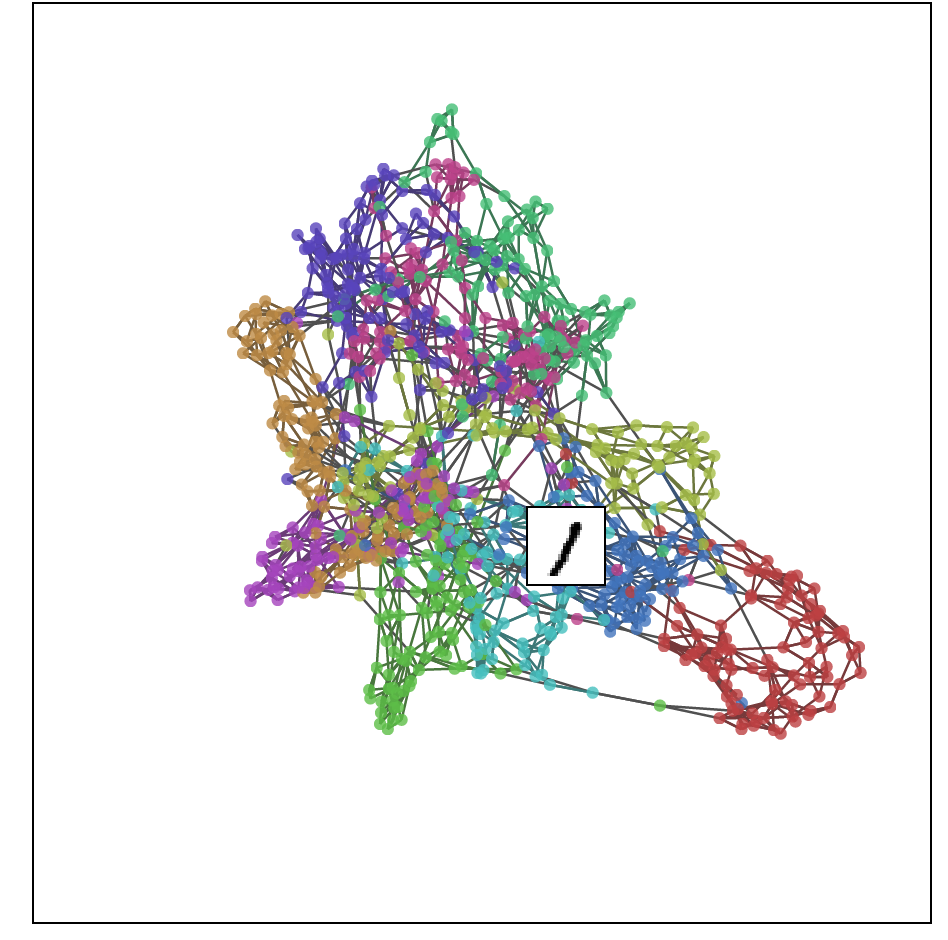
\includegraphics[width=0.3\textwidth]
    				{img/colah_nearest_neighbour.png} 
    			}}%
    			\caption{Three Nearest Neighbour Graph}%
    		\label{fig:3nn}
	\end{figure}	 	
 		
		\par 
		In order to do this a nearest neighbour graph is used; consider a graph $ ( \bm{V}, \bm{E}) $ of vertices $ \bm{V} $ and edges $ \bm{E} $ where the nodes are data points. One can arbitrarily choose the number of nearest neighbours to compare, but assuming three; if each point is connected to three other points within the original space, encoding the local structure clearly while forgetting about the rest. Using a standard force-directed graph all the points are treated as repelling charged particles, and the edges are springs - another visualisation is produced. Computing this gives us another cost function \cite{Olah2014b}:
		$$
			C = 
			\sum\limits_{i \neq j}
			\frac{1}{d(x_{i,j})} + 
			\frac{1}{2}
			\sum\limits_{ (i,j) \in \bm{E} } [ d(x_{i,j}) - d_{viz}(x_{i,j}) ]^2
		$$
		This representation has the extra useful property that it explicitly shows which points are connected to others, highlighting the local structure of the representation in two, or three, dimensions. This can help us discern the reason for certain apparent anomalies, such as a warped 6 misclassified as a 0, which may have appeared close together in the original space and now appear attached in the visualisation.			
		\par 
		A number of other techniques were reviewed by \cite{VanderMaaten2009} who describes \textit{Principle Components Analysis, PCA,} \cite{Hotelling33} - which finds the angle that spreads out the points the most in order to capture the largest variance possible, and \textit{Multidimensional Scaling} as seen above - as linear techniques that keep low-dimensional depictions of dissimilar points far away, but which fail to keep those data-points which are similar close together in the lower dimensional depiction.
 		
 	\begin{figure}[H]
    			\centering	
			{{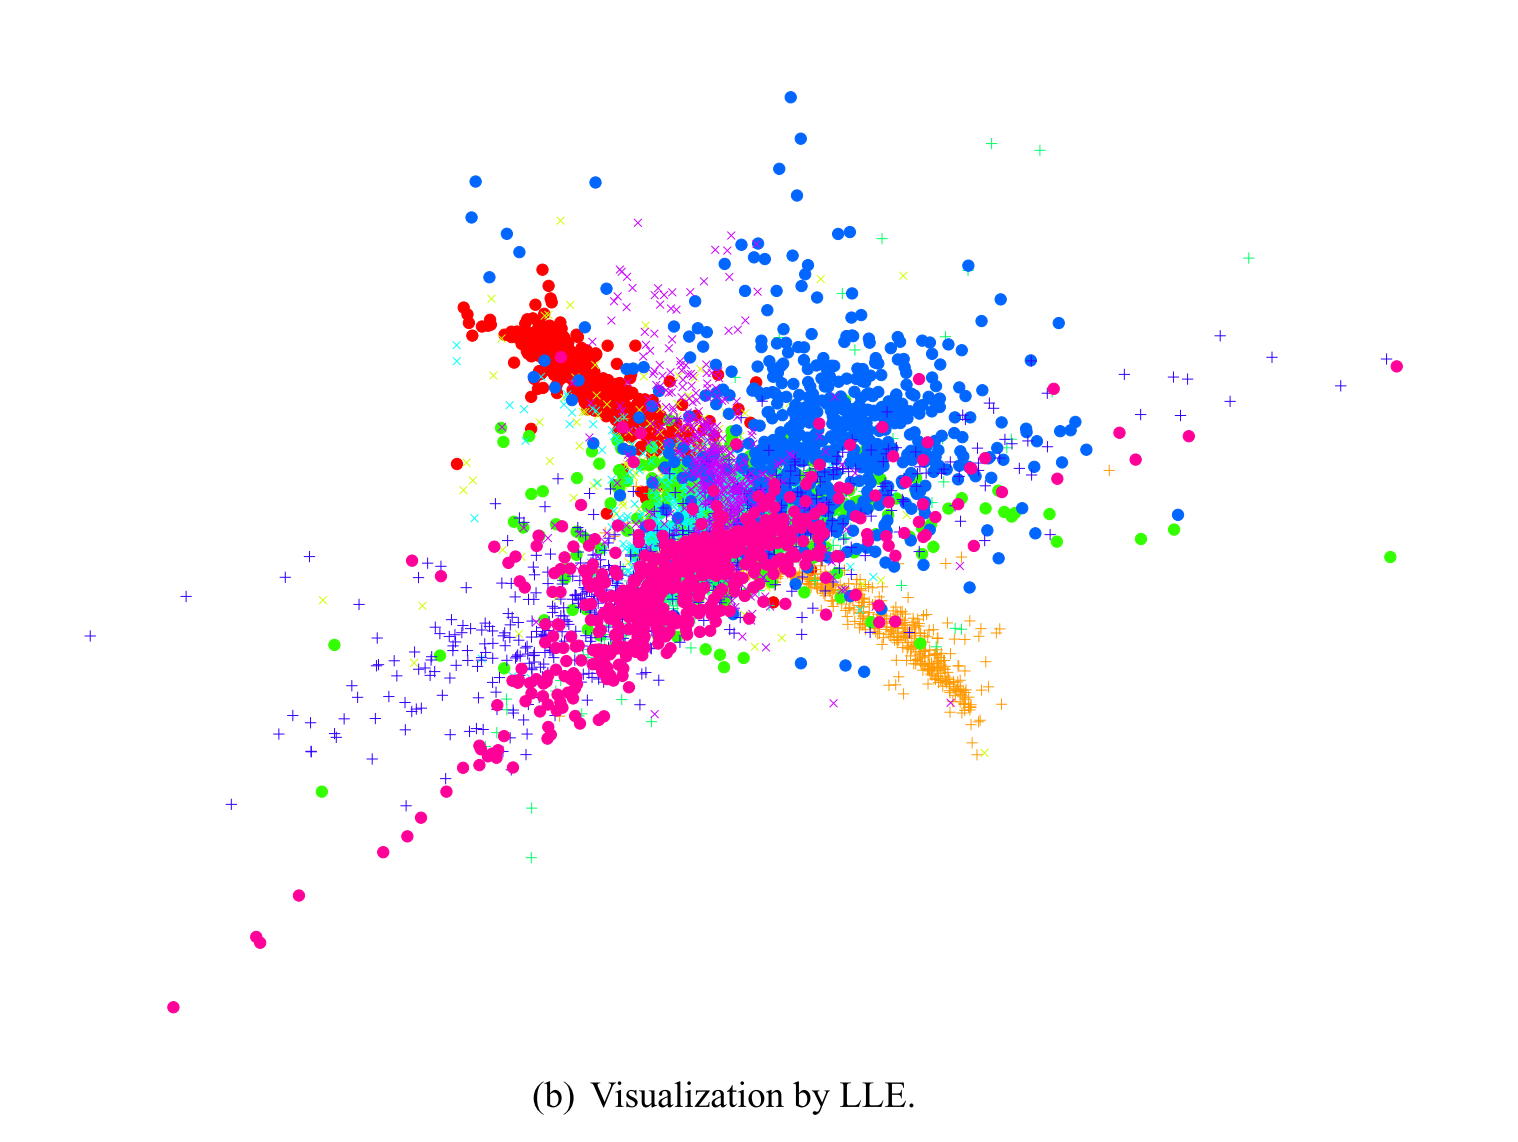
\includegraphics[width=0.3\textwidth]
    				{img/hinton_lle.png} 
    			}}%
    			\caption{Locally Linear Embedding}%
    		\label{fig:3nn}
	\end{figure}	 
 		
		\par 
		In addition to Sammons mapping described above, \cite{VanderMaaten2009} also sites a number of other non-linear dimensionality reduction techniques that aim to preserve the local structure of data including; \textit{Curvilinear Component Analysis} \cite{Demartines1995}, \textit{Stochastic Neighbour Embedding} \cite{Hinton2002}, \textit{Isomap} \cite{Tenenbaum2000}, \textit{Maximum Variance Unfolding} \cite{Weinberger2004}, \textit{Locally Linear Embedding} \cite{Roweis2000}, \textit{Laplacian Eigenmaps} \cite{Belkin2002}.

		\par 
		These techniques all perform well with artificial datasets, however are criticised for not being capable of retaining both local and global structure in a single data map. Even semi-supervised variants are not capable of separating simple datasets such as MNIST into it's natural clusters \cite{Song2007}. 
		\par 

	\begin{figure}[H]
    			\centering	
			{{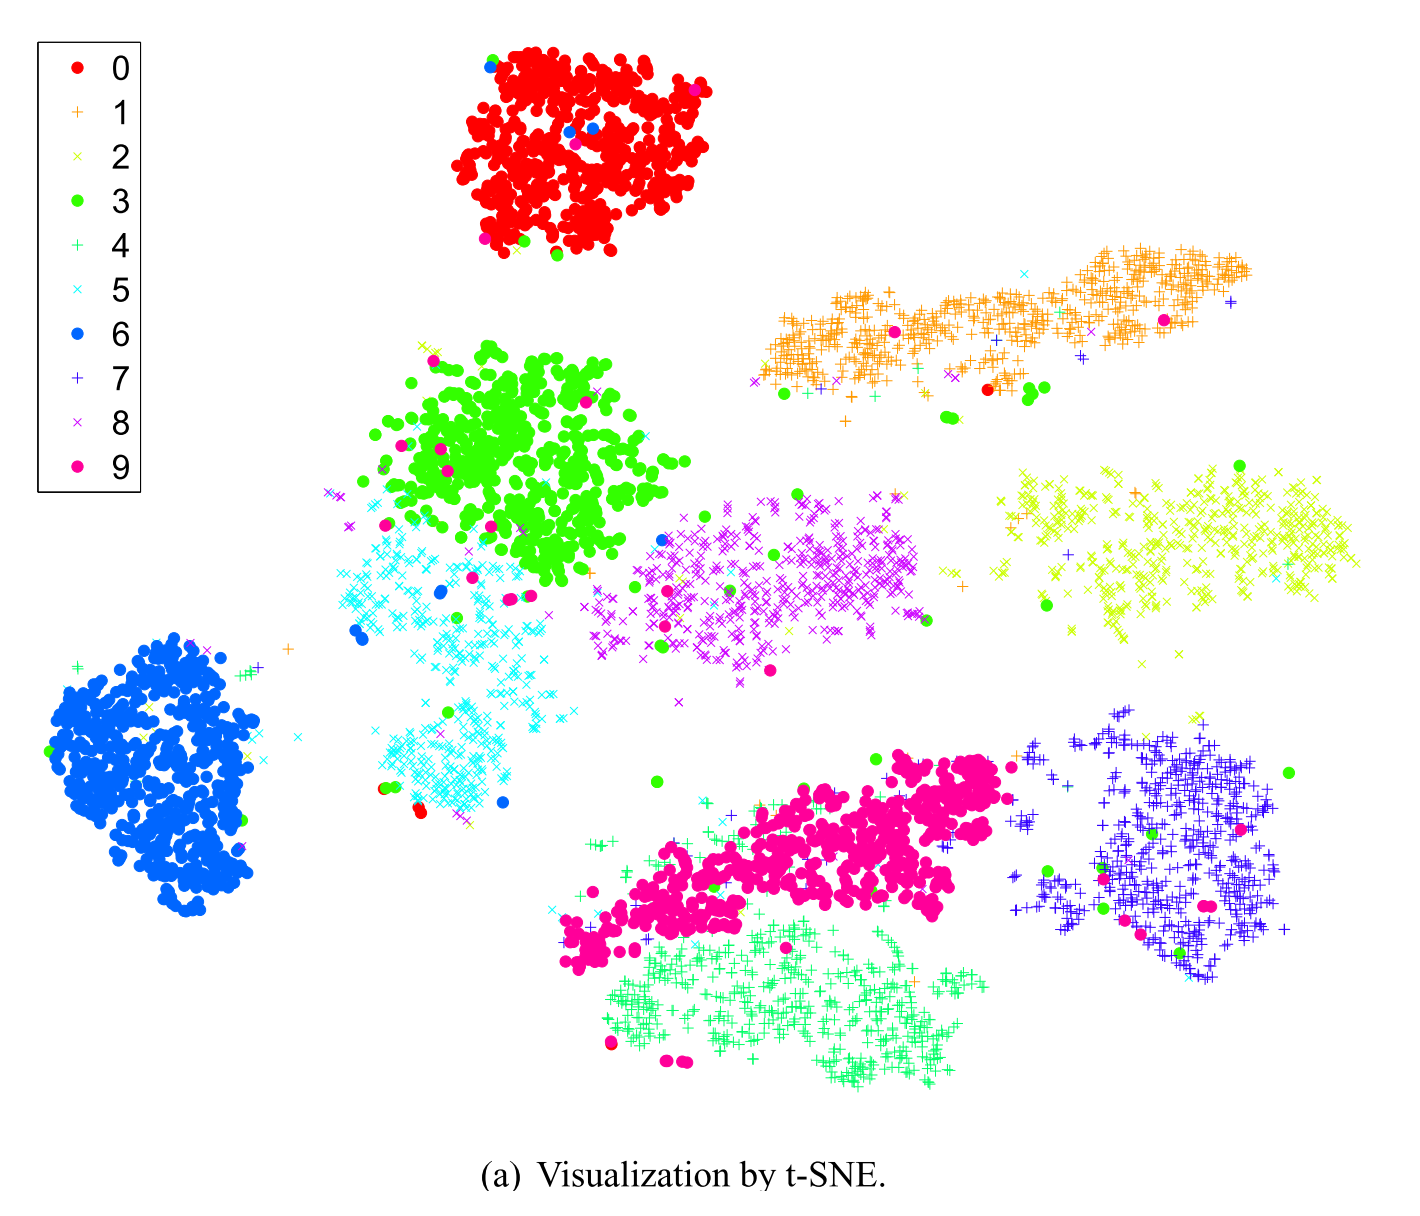
\includegraphics[width=0.3\textwidth]
    				{img/hinton_tsne.png} 
    			}}%
    			\caption{tSNE}%
    		\label{fig:3nn}
	\end{figure}	  		
 		
		More recently, and in direct challenge to those mentioned above, \textit{t-Distributed Stochastic Neighbour Embedding} \cite{Maaten2008} has provided a successful and widely used alternative for neural network researchers. t-SNE, as it is abbreviated, captures much of the local structure of high-dimensional data, while also revealing global structure such as the presence of clusters at several different scales.
		\par 
		t-SNE can therefore be viewed as preserving the topology of the data. t-SNE constructs for every data point a notion of which other points are it's `neighbours' and tries simultaneously to ensure that all points in the data have the same number of neighbours. t-SNE is a lot like the nearest-neighbour graph described above, however instead having a set number of neighbours connected by edges, and non-neighbours for which there are no connections, data points in the t-SNE reduction have a continuous spectrum of neighbours, for which they are neighbours to different, non-binary, extents. This makes t-SNE very powerful in revealing gloabl clusters and local subclusters within the data.
 		
	\begin{figure}[H]
    			\centering	
			{{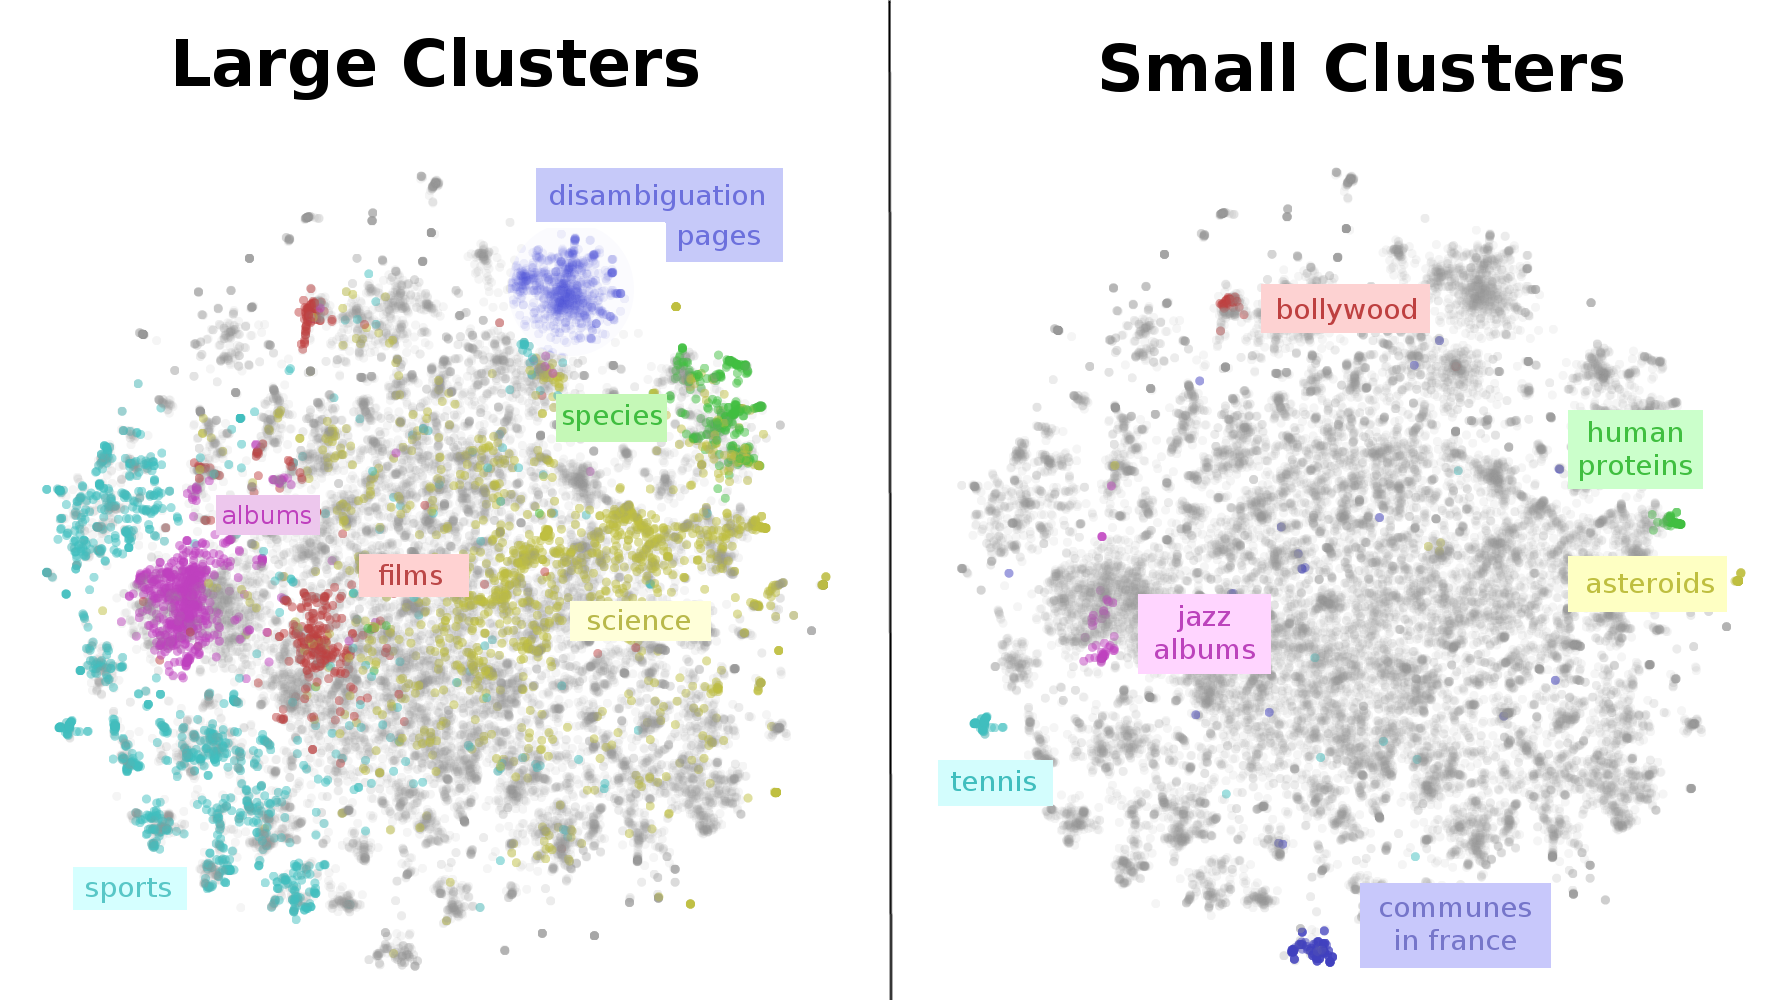
\includegraphics[width=0.3\textwidth]
    				{img/colah_wiki_large.png} 
    			}}%
    			\caption{Wikipedia visualised with t-SNE}%
    		\label{fig:wiki}
	\end{figure}	  	

		\par
		 The one downside of t-SNE is that it's prone to getting stuck at local minima, and due to it's increased complexity is more computationally expensive to run, such that changes cannot be made and visualised in real time on standard machines and can take any number of hours, or days even, to produce.  
		\par 
		t-SNE has been used to visualise MNIST to great success \cite{Maaten2008} and its retention of both global and local structure are clear when we examine clusters for patterns that emerge; such as with the ones, as they go from one angled variation across a spectrum to another with the cluster.
 		
 	\begin{figure}[H]
    			\centering	
			{{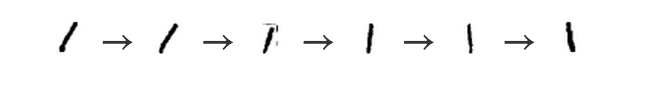
\includegraphics[width=0.3\textwidth]
    				{img/colah_tsne_distribution.png} 
    			}}%
    			\caption{Ones visualised by tSNE}%
    		\label{fig:wiki}
	\end{figure}	  
 		
		\par 
		Interestingly while a lot of these were designed for two dimensional representations of multi-dimensional data, they can significantly improved when visualised in three dimensions.
		\par 
		Not one of these dimensionality reduction techniques is superior. They are largely complimentary, and depending of the needs of the data-set and the visualisation scenario, they have different tradeoffs that can make one useful where another may not be. There is no exact mapping of high-dimensions to lower, each technique achieves some part of this mapping, but not all parts - trade offs must be made to preserve the most important properties given the context of the data-set and use scenario. PCA preserves linear structure, MDS preserves global geometry and t-SNE tries to preserve a topological neighbourhood structure. 
		\par 
	
	\subsection{ANN Visualisation: Representations}
		
		\subsubsection{Overview}
		Dimensionality reduction techniques provide useful tools for visualising data with greater than three dimensions - most neural networks. As seen above, they allow the user to explore both global and local patterns within their data visually, providing perhaps previously unseen insights into their data-set and in it's manipulations. 
		\par 	
		The structure that dimensionality reduction tries to preserve when translating to two, or three, dimensional space can be seen as a higher-order \textit{representation} of the data. It has been suggested that one reason for the success of neural networks is that they discover optimal representations of the data that allow for more accurate classification \cite{Hinton1986}. Therefore exploring these representations from a visual perspective might help researchers inspected and explore this space and it's here that they are likely to see which features are contributing to the learning, which intermediate concepts - such as higher-level features - are being created by the hidden layers. Importantly, these representations are likely to be distributed \cite{Hinton1986} such that each concept is encoded in the activations of any number of the networks nodes, making understanding these concepts a greater problem than simply understanding the decision surface on singular neurons, but one that requires representations across all nodes. Ultimately understanding these better should provide a method to guide the training process that is less situated in trial and error.
		\par 
		
		\subsubsection{Space Transformation}
	 	Representations are created to perform easier classification in the latter stages of a neural network. In order for the a network to classify the points as belonging to either one or the other it must seek to find a linear separation of the two \cite{Olah2014a}. 
		\par 
		In the input space the network requires a relatively complex line to divide two curves on a plane. However each new layer transforms the spatial data creating a new representation that is easier to classify with a simple hyperplane.
				
		\begin{figure}[H]
    			\centering	
    			\subfloat[No hidden layer]							{{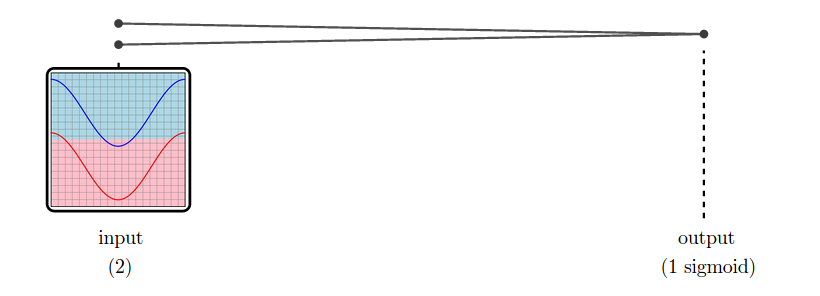
\includegraphics[width=7cm]
    				{img/colah_nonwarp.png} 
    			}}%
    			\qquad
    			\subfloat[Hidden Layer]
    			{{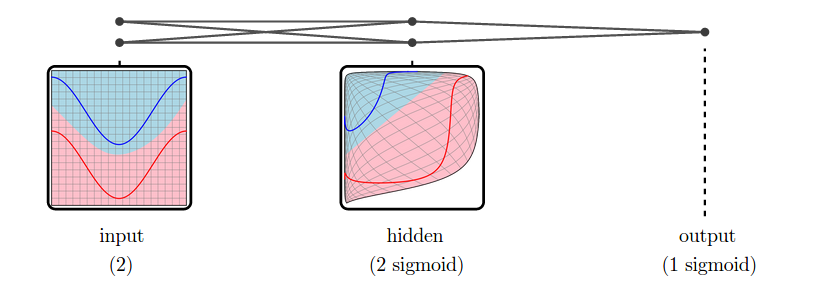
\includegraphics[width=7cm]
    				{img/colah_warp.png} 
    			}}%
    			\caption{Representations that warp the data}%
		\end{figure}		
		
		\par 
		In order for the data to be transformed to this new representation, it must undergo a sequence of manipulations. A tanh layer for example processing the function $ tanh(Wx + B) $ consists of; 
		\begin{itemize}
			\item a linear transformation by the weight matrix $ \bm{W} $
			\item a translation by the bias vector $ \bm{b} $
			\item and a point-wise application of the tanh activation function
		\end{itemize}
		Intuitively, what is occurring here is a stretching and warping of the space to make it easier to linearly divide and this can be seen above as well. It's important to note however that it does not cut, break or fold the space as it must retain it's `topological' properties \cite{Choi2005}.
		\par 
								
 		 \begin{figure}[H]
    			\centering													{{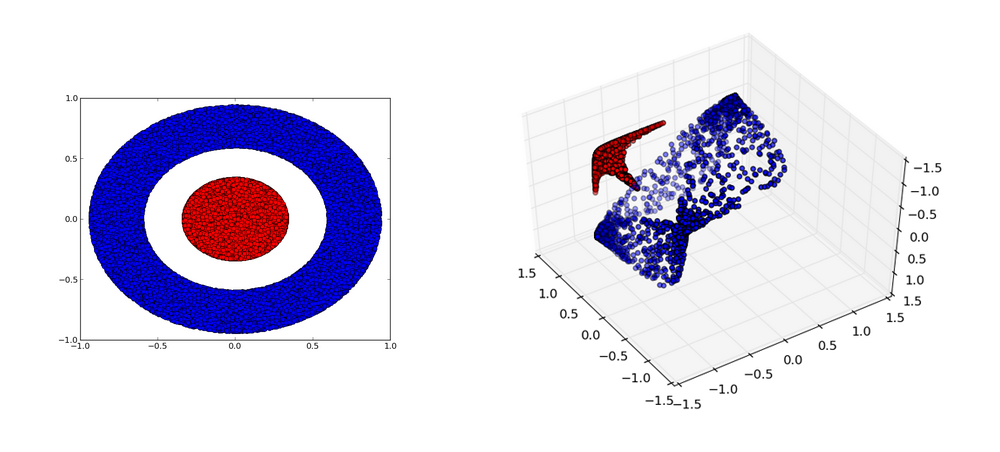
\includegraphics[width=0.6\textwidth]
    				{img/colah_circle} 
    				}}
    			\caption{Three Node Warping}%
    			\label{fig:studentprofile}
		\end{figure}
		
 		
		Another example, is one that cannot be warped simply in two dimensions, but requires a third, such as a circle within a circle:
		$$ 
		A = \text{ $ { xld(x,0) < 1/3 } $ }		
		B = \text{ $ { xl2/3 < d(x,0) < 1 } $ }
		$$ 
		It is impossible for a neural network to classify this without having a layer with greater than 3 hidden neurons. The requirement of the network to find a hyperplane that separates $ A $ and $ B $ in some final representation will not be possible no matter how the space is warped - the network requires an extra dimension. Visualisation demonstrates the network struggle to perform this. However, if we add a third  neuron, the problem becomes trivial - with a three dimensional representation of the data. This spatial transformation occurs in even more complex datasets with numerous dimensions \cite{Carlsson2008} such as images. however, while it is less easy to visualise these the intuition is useful and may lead to discovering appropriate ways of showing the same transformations in multi-dimensional space.
		\par 

		\subsubsection{Representation of word embeddings}
 		
 		 \begin{figure}[H]
    			\centering																			{{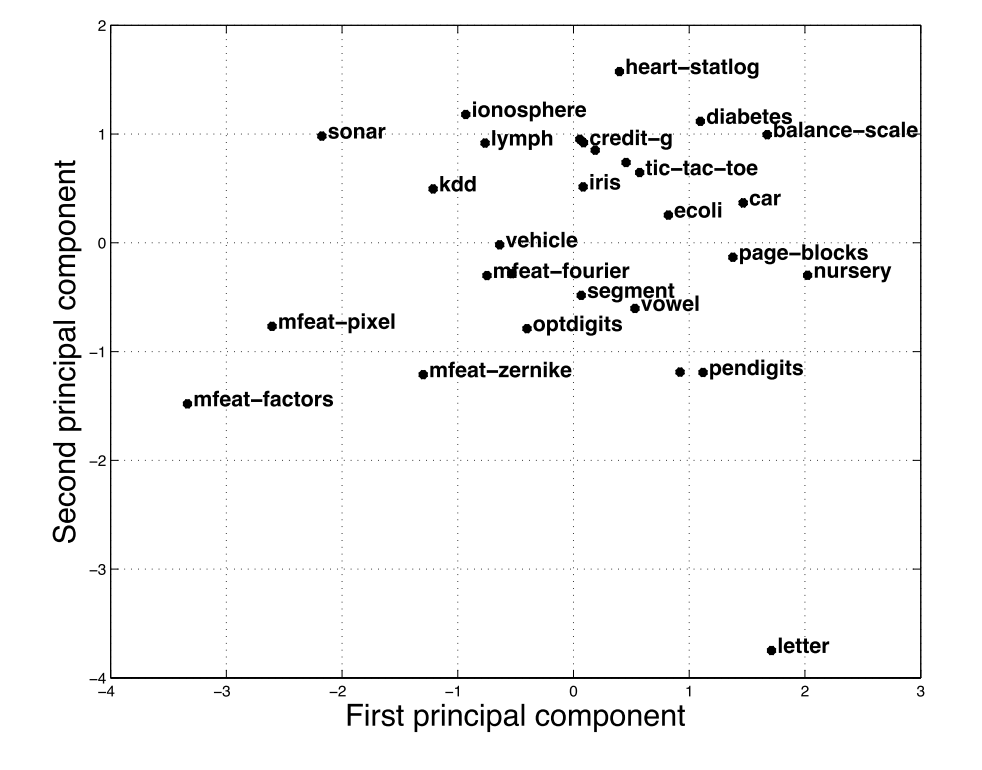
\includegraphics[width=0.6\textwidth]
    				{img/bardent_pca.png} 
    				}}
    			\caption{}%
    			\label{fig:pca}
		\end{figure}
		
 		
		A word embedding $ \bm{W : words \rightarrow \mathbb{R}^{n}} $ is a parametrized function that maps words to high-dimensional vectors \cite{Bengio2003}. If these are then passed through a learned representation $ \mathbb{R} $ of word-space we can classify the words.  		
		\par 
		In a word-embedding when you switch a word for its synonym or for another within its class - ``a few people sing well" versus ``a couple of people sing badly" - then while it appears the input has changed a lot, if $ \bm{W} $ maps synonyms (few $\rightarrow$ couple) and classes (well $\rightarrow$ badly) close together, then from the perspective in the representation $ \mathbb{R} $ very little actually changes.
		\par 

 		 \begin{figure}[H]
    			\centering																			{{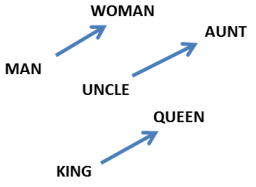
\includegraphics[width=0.6\textwidth]
    				{img/colah_word_embeddings.png} 
    				}}
    			\caption{}%
    			\label{fig:words}
		\end{figure}
		
		One way to get a feel for this word embedding is by using t-SNE to visualise the data. This displays words that are similar close together. The words appear to have have a physical representation - here analogies between words are encoded in the vector difference between words \cite{Olah2014c}, for example:
		$$
		W(``woman") - W(``man") \simeq W(``aunt") - W(``uncle") \simeq W(``queen") - W(``king")
		$$
		The intuition here is that the word embedding has learnt to categorise gender consistently, and it's clear to see that the model has likely learnt a gender representation.
 		\par  		
		 Translation from English into French sentences is achieved by understanding these representation's within two recurrent neural networks \cite{Sutskever2014} . The first processes the English, word by word, to produce a representation of it. The second takes the representation of the English sentence and sequentially outputs the translated words.

 		\begin{figure}[H]
    			\centering																			{{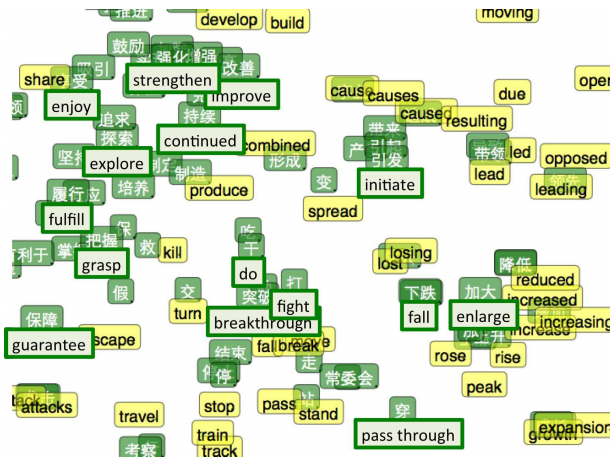
\includegraphics[width=0.6\textwidth]
    				{img/colah_language.png} 
    				}}
    			\caption{English and Chinese word representation plot}%
    			\label{fig:embeddings}
		\end{figure}	
		
		
		\par 
		An interesting discovery made possible by the visualisation of this system, is that the representation taken at the intersection of the two languages was heavily dominated by the first word of the sentence. Spotting this would have been near impossible in other non-visual depictions of the data, and it allows certain theories to be drawn about what the network is actually doing in order to process the information correctly. \cite{Olah2014} notes a number of possible deductions from this information.
		
		\subsubsection{Hidden Layer Representations}
 		
 		 \begin{figure}[H]
    			\centering																			{{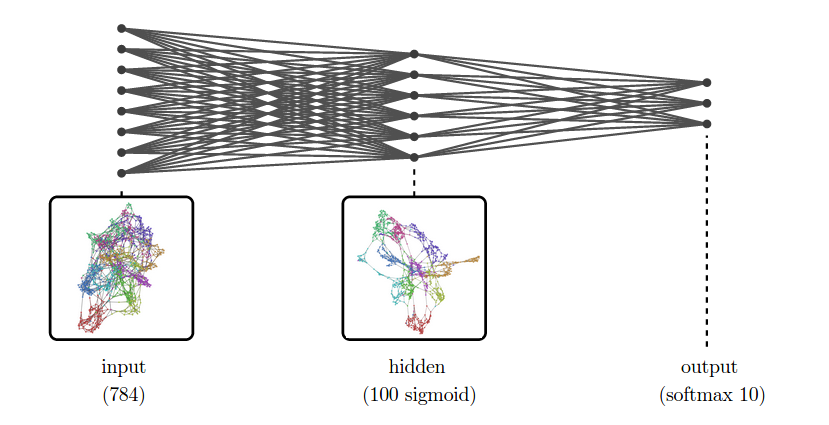
\includegraphics[width=0.6\textwidth]
    				{img/colah_mnist.png} 
    				}}
    			\caption{Force Directed Graph at input and hidden representation}%
    			\label{fig:fdg}
		\end{figure}	
		
		Another level of insights provided by representations can be attained by comparing representation's across layers. One interesting visual example of a representation, produced by \cite{Olah2014}, is of the MNIST dataset. A nearest neighbour, force-directed graph that is used to show classes which are fairly tangled and chaotic at the input, where it's easy to assume little classification. However by the next layer because the model has already been trained to distinguish digit classes, the hidden layer has learned to transform the data into an alternate representation that is easier to classify, and easier for a researcher to discern if the classification is performing as expected.				
		\par 
	
		\subsubsection{Transfer Function Representations}
		In addition to examining the representations at any given layer, it's possible to compare representations provided by different transfer functions. 
		\par 
		Each Neuron warps the space it interacts in rather differently. Using Principle Component Analysis as a dimensionality reduction technique, it becomes easy to understand this deformation of input space.
		\par 
		With a five unit sigmoid layer projected into three dimensions using PCA, its clear to see that the representation is very much like a cube. This intuitively makes sense, as sigmoid units tend to give values close to 0 or 1, and less frequently produce values in the middle. If the transformation is performed across the five dimensions with the sigmoid layer, then there ends up being a concentration at the corners and edges - thus creating a high-dimensional cube. 
		\par 
		
		\begin{figure}[H]
    			\centering												{{\includegraphics[width=0.4\textwidth]
    				{img/colah_relu.png} 
    			}}%
    			\qquad
    			{{\includegraphics[width=0.4\textwidth]
    				{img/colah_sigmoid.png} 
    			}}%
    			\caption{ReLU neuron versus Sigmoid neuron representation}%
		\end{figure}
 		
		If PCA is applied to a five unit ReLU layer, then a different geometric fingerprint is seen. The ReLU has a high probability of having zero activations - resulting in lots of points tending to the origin, or along the axes. Again in high-dimensions, this takes a physical representation and looks like a series of spikes originating from zero. 		
		\par 
		The interesting point to note is that very quickly it becomes possible to come to intuitive conclusions about how our data is being manipulated by the different functions. Far clearer certainly than if we were to simply look at the weights, activations and biases on a spreadsheet. 
		\par 
		
		\subsubsection{Isometries in Representations}
		
		\begin{figure}[H]
    			\centering												{{\includegraphics[width=0.25\textwidth]
    				{img/colah_flip01.png} 
    			}}%
    			\qquad
    			{{\includegraphics[width=0.25\textwidth]
    				{img/colah_flip.png} 
    			}}%
    			\caption{A flipped representation}%
		\end{figure}
		
		Visualised representations effectively form a geometric footprint of the transformed data. This is not the same every time we train the network and can change depending on small variables. This makes it likely that we could end up with several minor variations of the same dataset.
		\par 
		Sometimes a different representation means something significant, like learning a new characteristic of the data, and at other times the new representation is simply an insignificant transformation in isometries, like rotation or flipping - where nothing new is really learnt. It's important to reduce the chances of seeing these isometries as they can confuse what experts learn from the data.
		\par 
		What is required is a form of representation that encodes only meaningful differences. In dimensionality reductions, such as PCA or t-SNE, we are primarily concerned with distance between points as this holds the important notion of similarity and difference.
		\par 
		\cite{Olah2014} states that for any representation $ X $ there is an associated metric function, $ d_{x} $, which gives us the distance between pairs of points within that representation. For another representation $ Y $, $ d_{x} = d_{y} $ if and only if $ X $ is isometric to $ Y $. This is exactly the form with removal of isometries required.
		\par 
		The issue with $ d_{x} $ however is that it is a function on a very high-dimensional continuous space, caused by the need to consider the distance between functions as infinite dimension vectors. 
		$$
		D_X = \left[\begin{array}{cccc} 
		  d_X(x_0, x_0) & d_X(x_1, x_0) & d_X(x_2, x_0) & ... \\
		  d_X(x_0, x_1) & d_X(x_1, x_1) & d_X(x_2, x_1) & ... \\
		  d_X(x_0, x_2) & d_X(x_1, x_2) & d_X(x_2, x_2) & ... \\
		  ... & ... & ... & ... \\ 
		\end{array} \right]
		$$
		Here we require another application of dimensionality reduction - again reapplying t-SNE, PCA or some other technique. \textit{meta-SNE} is a recently introduced variation of t-SNE by \cite{Olah2014} that performs the above flattening of distance matrices. This meta-SNE visualisation of distance shows how much representations disagree about which points are similar and which are different - allowing us to have quick overview of when a network has learnt an entirely new representation or not. This moves the position up from looking at representations, to the space of representations.
		\par 
		
		\begin{figure}[H]
			\centering
						
    			\includegraphics[width=0.40\textwidth]{img/colah_meta_sne.png}
\caption{Meta-SNE representation $\rightarrow$ t-SNE representation $\rightarrow$ MNIST digit}
 		\end{figure}
 		
		It is possible here that this space could be used to see how current model representations compare to other `landmark' representations from past experiments. If the models first layer representation is in the same place as a really successful model, then that's likely to be positive. If however it's tending towards a cluster that had some specific poor quality, the researcher would know to adjust for this too. This provides us with some qualitative feedback during the training of the neural network. 
		


\subsection{Existing Visualisation Software}

		\begin{figure}[H]
    			\centering	
		{{\includegraphics[width=18cm]
    				{img/rui_wang_vis_overview} 
    			}}%
    			\caption{Overview of visualisation software by Rui Wang}%
    		\label{fig:studentprofile}
		\end{figure}
		
	There are a number of tools for visualising elements of what we have discussed above, below is a short summary of some commonly used tools and their features derived in part from \cite{Wang2015}:
	\par 
		\textbf{D3.js} is an open source library built in JavaScript and is designed to use the capabilities of web standards such as CSS3 (Cascading Style Sheets), HTML5 and SVG (Scalable Vector Graphics). It was created by researchers from Stanford University's Visualisation Group. It has implementations of animations, interactions and other  complex and dynamic visualisation types. It addresses many of the challenges derived from visualisation on the web by putting emphasis on the efficient manipulation of HTML elements. It's kernel uses pre-built JavaScript functions to select elements, create SVG objects as well as style them, add transitions or dynamic effects.
		\par
		\textbf{JFreeChart} is a free Java Library for developing graphs and charts. Although it is not open-source it is potentially one of the most widely used libraries in Java for charting. The library supports most common chart types and its API includes interactive features such as tool tips, colour gradients, drop-shadows and zooming. 
		\par 
		\textbf{Google Charts} is a free, non open-source, JavaScript-based visualisation package. Developed by Google, it allows users to embed different kinds of charts and maps in their web pages. The most common way to use Google Charts is by embedding the JavaScript a web-page. Handily, the charts can read data directly from a web page, from a database or even stored in a Google Spreadsheet. 
		\par 
		\textbf{matplotlib}
		is an open source library written in python and is aimed at creating primarily 2D plots. These plots are embeddable in a graphical user interface (GUI) for application development and its code is easy to understand and extend. A large user community has developed a lot of powerful tools on the back of it.
		\par 
		\textbf{Gephi}
		is an open source Java based platform for visualising and manipulating large graphs. It is often regarded as the Photoshop for networks and graphs as users can interact with the graph representation and manipulate its structure, shape and colour. Gephi has a built-in OpenGl engine and is therefore able to visualise and interact with very large networks in real-time. Additionally Gephi's software architecture is built on top of the `NetBeans' platform, meaning it can be extended or reused easily through well-written APIs.
		\par 
		\textbf{Graphviz} is an open source software package created by AT\&T for visualising connectivity graphs. It contains many standard graph layouts which can be used via a programming interface, command line tools, GUIs and web browsers.
		\par 
		\textbf{Sigma.js}
		is another source JavaScript library, it is backed by the company `Sciences-Po Medialba'. The library is dedicated to graph drawing, using either HTML5 canvas or WebGL. It has been specifically designed to interactively display graphs exported from other software in real time. It is lightweight and doesn't require external dependencies. The default configuration of Sigma.js provides a variety of built-in features, like HTML5 web canvas and WebGL renderers, mouse and touch support. At its core it is a rendering engine and does not include many graph related features out of the box such as layout and clustering.
		\par 
		\textbf{mxGraph}
		is a family of libraries that provide features for displaying interactive diagrams and graphs. It provides a range of commonly required functionalities to draw, interact with and associate a context with a diagram. It can represent nodes in shapes, images, vector drawings and animations. Developers can then interact with the generated diagrams through a series of actions like dragging or cloning of cells, resizing and reshaping, connecting and disconnecting, drag and dropping, or in-place editing. It also offers a flexible API for developers to program the behaviour of these interactions. 
		\par 
		\textbf{DeepViz} was produced by a group of Berkeley researchers\cite{Bruckner2013} in 2013, and aimed to provide an interactive visualisation system specifically for CNNs. It is built on a featurization system, Decaf\cite{Donahue2013} that provides a number of features that allow users to explore convolutional filters as bitmaps, view side-by-side comparisons of weight matrices, see a time line visualisation of their model, and view class output accuracy as a confusion matrix. It is a python implementation with a GUI interface. While it appears to provide a lot of useful tools for ANNs, it is rudimentary and lacks any interaction functionality that would transform it from a tool used to produce visualisations, into a tool to explore through visualisation. It is however an opensource project specifically targeted for CNNs.
		\par 
		\textbf{Expresso}
		Expresso, is a GUI tool that has been built on top of Caffe, a popular framework used to develop neural networks. Built by a team of researchers from the Indian Institute of Science \cite{Dholakiya2015} who describe it as a ``wizard-like graphical interface which guides the user through various common scenarios." It includes number of features such as Caffe data import, construction of a Caffe model and GUI for training of deep networks, analysis and basic visualisation of experiments using bitmaps. Like DeepViz, it is also built on top of the open source featurization system Decaf \cite{Donahue2013}. Unfortunately with so much functionality, it is a clunky beta version at present.
		\\\
		The on-going explosion of large datasets presents a significant challenge to existing visualisation libraries. Since most of the libraries focus on handling data sets of small or intermediate size, the majority of them are not designed with scalability in mind. While the parallel computing and GPU-based implementations allow visualisation libraries to access significant compute, the approach often requires specific knowledge to understand the platform or parallelisation mechanism.
		\par 
		Additionally, most of the existing visualisation libraries fall pray to the classic problem of a `do it all' approach, aiming to please everyone while not fully pleasing anyone. They also are greatly influenced by the technologies they are written in, and it's incredibly hard to produce visualisations across language. Recently, more language agnostic means of data transformation have appeared due to browser led development, passing data through RESTful APIs, JSON objects, simple .CSV documents, or interacting with tabling tools such as exported from googlesheets. This is likely to be the path that future visualisation libraries take.

\section{Progress Summary}
	\subsection{Investigation and Data Collection}
		\subsubsection{Survey}
		Deep Neural Networks sometimes contain hundreds of parameters which one can tweak, and a vast array of elements that may be added or subtracted from the standard network architectures described earlier.
		\par 
		While it would be great to visualise everything in this project - unfortunately this isn't feasible, and so in order to establish which areas to start on, a survey has been created to distribute amongst the vast deep learning community. 
		\par 
		There are three components to the survey:
		\begin{itemize}
			\item \textbf{Working Environment:}
		In order to assess which areas would be most effective in terms of increasing efficiency of work, the aim is to find out which broad areas of working with DNNs take up most time.
		\par 
		To ensure that any tools developed throughout this project are suitable to both the academic and practitioner communities, the survey aims to find out which packages and languages people are most familiar with.
			\item \textbf{Training Methods}
		In order to develop visualisations that are immediately useful, the survey aims to find out what the most frustrating problems are for the researcher, and to avoid duplication of what exists already - ask if they have found effective solutions to these problems.
		\par
		Two other questions aim to diagnose which parameters are \textit{A} most important to producing a working network, and \textit{B} most commonly tweaked.
			\item \textbf{Visualisation}
		The section begins by showing five images of DNNs being visualised in a variety of different ways, with the aim of clarifying any misunderstandings about what it means to visualise these networks. As a bonus, the survey uses these to deduce which appear to be most useful - each is in it's own distinct category of visualisation.
		\par 
		Having established what visualisations may be possible, the survey continues to ask more focussed questions aimed at understanding if people have had prior experience with visualisation, where and why they think they would use it, and how they would like to interact with it if such a thing existed. This information is both explicitly asked for an implicitly deduced by a series of free-text and selection questions.
		
		\end{itemize}
		\par
		
		\subsubsection{Categorising and Understanding Academic Visualisations}
		One area within the field of Deep Learning that uses vast amounts of visual material, if aggregated, is across the academic body of research. 
		\par 
		Graphs, charts, 3D planar surfaces, diagrams, morphed images, and more, all contribute a significant amount to helping readers understand, and writers explain new concepts and cutting edge research. It seems then, to be a good place to start examining if one wants to understand the types of things the community chooses to remove from mathematical syntax, and place in a visual form.
		\par	
		The body of visualisations collected is approximately 200, and growing. Each visualisation is categorised under the following headings:
		\begin{itemize}
			\item \textbf{The type of visualisation:} 				This information will provide a useful data point about the types of visualisation most understood and favoured by the community. This will make it far easier to produce visualisations that have the right level of explanation required to make any new visualisation types easy to process.
			\item \textbf{Any comparisons made:} 
			This will provide invaluable information about which parameters researchers most often use to make decisions about performance, and ultimately lead to change in their models. Understanding this will help to ensure that visualisations produced for the case-study experiment are not 'overfitting' to the case-study, and are actually still useful to the community as a whole.
			\item \textbf{Any axis-labelling, or annotations:}
			Similar to above, this will provide an understanding of the features and scales that the community most values. For example, error rate as a percentage features heavily against time - but also occasionally features against other variables. Again, this provides a useful reference point as to what the community of researchers is most interested in, and allows this project to progress without needed to be an expert in the field.
		\end{itemize}
		\textit{Please see appendix A}
		
		\subsubsection{Collecting Iterative Visualisations: Sketches}
		The process of acquiring this information has only just begun, however it will provide an invaluable insight into forms of visualisation that are not confined to those that have been iterated upon and refined for the purpose of publication. 
		\par 
		The data collected in this research are sketches, quick diagrams and `hacky' visualisations made by software - ideally accompanied by some description of what the researcher was trying to explain, or understand.
		\par 
		With this information, it will become far clearer what is required in terms of content for visualisations made for understanding and exploration as opposed to visualisations made for explanation. Ultimately this information should allow visualisation to be targeted towards helping researchers make key decisions. 
	\subsection{Understanding Literature}
	Thus far; a number of papers have been read, a number of tutorials undertaken, and a number of online lectures watched - both in the discipline of visualisation and in working with deep neural networks.
	\subsection{Clarifying Goals}
	The goals set out when proposing this project appeared to be quite clear. However, as with any project, the more understanding you have of a topic - the more you realise you didn't understand before. This has been made incredibly clear, and even early research into what would be valuable for those implementing deep neural networks has changed the course of how this project will work. Hopefully it is more on the right tracks now.

\clearpage
\section{Plan}

	\subsection{Learning to Implement}
	The month of June will be spent learning the follow software with a first prototype ideally ready in the first weeks of July.
		\subsubsection{Node Server}
		Node.js is a platform built on Chrome's JavaScript runtime for easily building fast, scalable network applications. Node.js uses an event-driven, non-blocking I/O model that makes it lightweight and efficient, perfect for data-intensive real-time applications that run across distributed devices.\cite{Dahl2009}
		\par 
		In 2011, a package manager was introduced for Node.js library, called npm. The package manager allows publishing and sharing of open-source Node.js libraries by the community, and simplifies installation, updating and uninstallation of libraries \cite{Dahl2009}.
		\par 
		These features make Node.js an ideal option for developing a visualisation tool that will hopefully be used by a vast number of researchers. Indeed, npm is already a common method of sharing proprietary DNN software within the DL community. 
		\subsubsection{D3 Visualisation Library}
		D3.js, or Data Driven Documents, is a JavaScript library for producing dynamic, interactive data visualizations in web browsers.
		\par 
		D3 allows the binding of arbitrary data to a Document Object Model (DOM), and then apply data-driven transformations to the document. For example, you can use D3 to generate an HTML table from an array of numbers. Or, use the same data to create an interactive SVG bar chart with smooth transitions and interaction.\cite{Bostock2011a}.
		\par
		D3 is extremely fast at supporting large datasets, making it ideal for working with often data-intensive neural networks. The dynamic behaviours enabled for interaction and animation make it highly suited to the task of exploring visualised data with the aim of deriving new insights from such data.
		\subsubsection{Working with Neural Networks}
		For this project, one deep learning library will be explored in greater detail that the others. This should allow experimentation to progress quickly, and it assumed that visualisation that are useful for one library can be transferred across to another with \textit{relative} ease.
		\par 
		Theano is a Python library that allows users to define, optimize, and evaluate mathematical expressions involving multi-dimensional arrays efficiently. Theano is often used alongside the lightweight library, or wrapper, Lasagne - which provides a compact interface for developing neural networks, and supports a number of different architectures.
		
	\subsection{Investigation and Data Collection}
	Throughout this project, it will be important to continually reflect on the usefulness of visualisations produced. In order for this to occur, two approaches will be taken; a depth first research model, and a breadth first research model.
		\subsubsection{Depth First Research}
		Depth First Research: also known as 'Concierge Service' within other industries. 
		\par		
		This process tailors the project to the needs either one researcher, or a small number of individuals. It ensures that a useful product is produced for this small subset before developing out for a wider, potentially more varied user-base.
		\par
		In this instance this is likely to be a small group of Imperial Researchers. The initial task is to provide each of these researchers with bespoke visualisations for a range of data they deem to be useful. Next, the goal will be to provide them with a package that automates this process such that they can produce the visualisation within their existing work flow.
		\subsubsection{Breadth First Research}
		Breath First Research: also know as 'Market Investigation' in other industries.
		\par
		This process involves reaching out to the wider community of researchers, practitioners and hobbyists. This has already begun, and will progress as follows:
		\par 
		\textbf{Survey} A survey of X community members will be collated and analysed to assess users needs.
		\par 
		\textbf{Alpha-Testing} An early prototype will first be tested by the participants in the Depth First Research group. The product will then be improved upon before being released to a larger sample group.
		\par
		\textbf{Beta-Testing} With a more developed prototype, this will now be tested by those who agreed to be early-adopters from the survey.
		\par
		\subsubsection{Limitations}
		\begin{itemize}
			\item Project Bias with Depth First Research: the project may develop visualisation that are too particular to the research group.
			\item Survey Result Bias in Community: it is possible that only a limited number of proactive members will respond, or those with a real need for visualisation - thus again introducing a bias to the development of the project.
		\end{itemize}

	\subsection{Experiment 1: Explanation - Visualising MNIST}
	This experiment will centre around producing visualisations for the well understood dataset - MNIST.
	\par 
	The aim will be to create an array of different visualisations that reflect the dataset, and those that have already been produced within the academic literature surrounding DNNs.
	\par 
	The experiment should reveal which parts of DNNs are easy to visualise, which appear to be most useful, and should also provide the basis for an implementation to be used with latter experiments.  

	\subsection{Experiment 2: Exploration - Visualising another well known dataset}



	\subsection{Experiment 3: Exploration - Visualising Energy Disaggregation: Auto Encoders and RNNs}
	This will test the previously created visualisation techniques from the MNIST experiment on a live, and potentially more dirty data-set.
	\par 
	The aim will be to create a set of visualisations that reflect the data, but also that provide novel insights or more efficient insights.
	\par 
	This experiment should further develop the tool being used, and refine the selection of visualisations to a set that provide information in a clear and useful manner. \cite{Shoresh2011} \cite{Maaten2008}

\clearpage

\bibliography{background_bibliography}
\bibliographystyle{agsm}

%\addcontentsline{toc}{section}{References}
\clearpage
\appendix
	\section{Classifying Academic Visualisations}
		 \begin{figure}[H]
    			\centering	
	{{\includegraphics[width=16cm]
    				{img/explanation_research_02} 
    			}}%
    			\caption{Sample of Classifying Image Data}%
    		\label{fig:studentprofile}
		\end{figure}

		
		\begin{figure}[H]
    			\centering	
		{{\includegraphics[width=16cm]
    				{img/explanation_research_01} 
    			}}%
    			\caption{Sample of Classifying Image Data}%
    		\label{fig:studentprofile}
		\end{figure}
		
		
		\begin{figure}[H]
    			\centering	
		{{\includegraphics[width=14cm]
    				{img/exploration_data_rotate} 
    			}}%
    			\caption{Sample of Analysis of Image Data}%
    		\label{fig:studentprofile}
		\end{figure}
		
		\clearpage



\end{document}

